%% ============================================================================
%%  Trabajo de Titulación — Universidad Tecnológica Indoamérica
%%  Autor: Fernando José Ochoa Cobeña
%%  Compilar:  compilar.bat   (pdflatex → bibtex → pdflatex ×2)
%% ============================================================================
\documentclass{tesis-uti}

%% ============================================================================
%%  configuracion.tex — datos del trabajo de titulación
%%  Autor: Fernando José Ochoa Cobeña  |  Tutora: Ing. Fátima Adriana Avilés Castillo, Mg.
%% ============================================================================

%% --- Institución -----------------------------------------------------------
\newcommand{\Universidad}{UNIVERSIDAD TECNOLÓGICA INDOAMÉRICA}
\newcommand{\UniversidadNombre}{Universidad Tecnológica Indoamérica}
\newcommand{\UniversidadPortada}{UNIVERSIDAD TECNOLÓGICA\\INDOAMÉRICA}
\newcommand{\Facultad}{FACULTAD DE INGENIERÍAS}
\newcommand{\Carrera}{INGENIERÍA EN TECNOLOGÍAS DE LA INFORMACIÓN}
\newcommand{\CarreraNombre}{Tecnologías de la Información}
\newcommand{\TituloAObtener}{Ingeniero en Tecnologías de la Información}
\newcommand{\Repositorio}{Repositorio Digital Institucional (RDI-UTI)}
\newcommand{\Ciudad}{AMBATO}
\newcommand{\CiudadTexto}{Ambato}
\newcommand{\Pais}{ECUADOR}
\newcommand{\Anio}{2026}

%% --- Trabajo ----------------------------------------------------------------
%% TÍTULO REGISTRADO. Por indicación del tutor el tema no se modifica; el trabajo
%% se ajusta al tema (ver «Relación con el tema del trabajo» en el Capítulo I).
\newcommand{\Tema}{MODELOS DE MACHINE LEARNING PARA LA PREDICCIÓN DE INDICADORES DE SALUD PÚBLICA APLICANDO LA METODOLOGÍA OSEMN A PARTIR DE DATOS ESTRUCTURADOS EN TUNGURAHUA}
\newcommand{\TemaTexto}{Modelos de Machine Learning para la predicción de indicadores de salud pública aplicando la metodología OSEMN a partir de datos estructurados en Tungurahua}
\newcommand{\TemaIngles}{MACHINE LEARNING MODELS FOR THE PREDICTION OF PUBLIC HEALTH INDICATORS APPLYING THE OSEMN METHODOLOGY FROM STRUCTURED DATA IN TUNGURAHUA}
\newcommand{\Modalidad}{Trabajo de Titulación modalidad Trabajo de Integración Curricular}

%% --- Autor y tutora ------------------------------------------------------------
\newcommand{\Autor}{Fernando José Ochoa Cobeña}
\newcommand{\Tutor}{Ing. Avilés Castillo Fátima Adriana, Mg.}
\newcommand{\TutorAprobacion}{ING. AVILÉS CASTILLO FÁTIMA ADRIANA, MG.}
\newcommand{\Cedula}{0750919227}
\newcommand{\Direccion}{Tungurahua, Ambato, La Península}
\newcommand{\Correo}{fochoa2@indoamerica.edu.ec}
\newcommand{\Telefono}{0997872246}

%% --- Fechas ------------------------------------------------------------------
\newcommand{\FechaAutorizacion}{a los 09 días del mes de abril de 2026}
\newcommand{\FechaAprobacion}{17 de septiembre de 2026}

%% --- Tribunal (PENDIENTE: nombres reales de los lectores) --------------------------
\newcommand{\MiembroA}{[Nombres y apellidos del miembro de tribunal 1]}
\newcommand{\MiembroB}{[Nombres y apellidos del miembro de tribunal 2]}
                 % datos del trabajo (autor, tema, etc.)

\hypersetup{pdftitle={\TemaTexto},pdfauthor={\Autor}}

\begin{document}

%% --- Preliminares -----------------------------------------------------------
%% Portada (sin número de página)
\begin{titlepage}
  \thispagestyle{empty}
  \setlength{\parskip}{0pt}
  \centering
  \vspace*{8.5mm}
  
\includegraphics[width=21mm]{figuras/logo-uti.png}\par
  \vspace{1mm}
  {\Large\bfseries\UniversidadPortada\par}
  \vspace{4mm}
  {\Large\bfseries\Facultad\par}
  \vspace{2mm}
  {\large\bfseries\Carrera\par}
  \vspace{1mm}
  \begin{flushleft}
    {\color{black!35}\rule{\textwidth}{0.4pt}}\par
    \vspace{-1mm}
    \hspace*{6.2mm}\textbf{TEMA:}\par
    \vspace{-1mm}
    {\color{black!35}\rule{\textwidth}{0.4pt}}\par
    \vspace{-3mm}
    \noindent{\large\bfseries\setstretch{1.2}\Tema\par}
    \vspace{-1.5mm}
    {\color{black!35}\rule{\textwidth}{0.4pt}}\par
    \vspace{1mm}
    \hspace*{6.2mm}\Modalidad\par
    \vspace{5mm}
    \noindent\textbf{Autor(a)}\par
    \noindent\Autor\par
    \vspace{1.5mm}
    \noindent\textbf{Tutor(a)}\par
    \noindent\Tutor\par
  \end{flushleft}
  \vspace{9mm}
  \Ciudad{} – \Pais\par
  \vspace{2mm}
  \Anio\par
\end{titlepage}

\preliminares
%% Autorización de repositorio digital (texto en cuerpo 10.95 pt, como el modelo)
\clearpage
\titulopreliminar{Autorización de Repositorio Digital}
\begingroup\small
Yo, \Autor, declaro ser autor del Trabajo de Titulación con el nombre
``\TemaTexto'', como requisito para optar al grado de Ingeniero/a en
\CarreraNombre{} y autorizo al Sistema de Bibliotecas de la
\UniversidadNombre, para que con fines netamente académicos divulgue esta obra
a través del \Repositorio.

Los usuarios del RDI-UTI podrán consultar el contenido de este trabajo en las
redes de información del país y del exterior, con las cuales la Universidad
tenga convenios. La \UniversidadNombre{} no se hace responsable por el plagio o
copia del contenido parcial o total de este trabajo.

Del mismo modo, acepto que los Derechos de Autor, Morales y Patrimoniales,
sobre esta obra, serán compartidos entre mi persona y la \UniversidadNombre,
y que no tramitaré la publicación de esta obra en ningún otro medio, sin
autorización expresa de la misma. En caso de que exista el potencial de
generación de beneficios económicos o patentes, producto de este trabajo,
acepto que se deberán firmar convenios específicos adicionales, donde se
acuerden los términos de adjudicación de dichos beneficios.

Para constancia de esta autorización, en la ciudad de \CiudadTexto,
\FechaAutorizacion, firmo conforme:

\vspace{6mm}
\noindent\textbf{Autor:} \Autor\par
\vspace{2mm}
\noindent\textbf{Firma:}\par
\vspace{2mm}
\noindent\textbf{Número de Cédula:} \Cedula\par
\vspace{2mm}
\noindent\textbf{Dirección:} \Direccion\par
\vspace{2mm}
\noindent\textbf{Correo Electrónico:} \Correo\par
\vspace{2mm}
\noindent\textbf{Teléfono:} \Telefono\par
\endgroup

%% Aprobación del tutor
\clearpage
\titulopreliminar{Aprobación del Tutor}
En mi calidad de Tutor del Trabajo de Titulación ``\TemaTexto'', presentado por
\Autor, para optar por el Título de \TituloAObtener.

\vspace{4mm}
\begin{center}\bfseries CERTIFICO\end{center}
\vspace{2mm}

Que dicho Trabajo de Titulación ha sido revisado en todas sus partes y considero
que reúne los requisitos y méritos suficientes para ser sometido a la
presentación pública y evaluación por parte del Tribunal revisor que se designe.

\vspace{10mm}
\CiudadTexto, \FechaAprobacion

\vspace{22mm}
\lineafirma{\TutorAprobacion}

%% Declaración de autenticidad
\clearpage
\titulopreliminar{Declaración de Autenticidad}
Quien suscribe, declaro que los contenidos y los resultados obtenidos en el
presente Trabajo de Titulación, como requerimiento previo para la obtención del
Título de \TituloAObtener, son absolutamente originales, auténticos y
personales y de exclusiva responsabilidad legal y académica del autor.

\vspace{10mm}
\CiudadTexto, \FechaAprobacion

\vspace{22mm}
\lineafirma{\Autor\\\Cedula}

%% Aprobación de lectores
\clearpage
\titulopreliminar{Aprobación de Lectores}
El Trabajo de Titulación ha sido revisado, aprobado y autorizada su impresión y
empastado, sobre el Tema: \textbf{\Tema}, previo a la obtención del Título de
\TituloAObtener, reúne los requisitos de fondo y forma para que el estudiante
pueda presentarse a la sustentación del Trabajo de Titulación.

\vspace{10mm}
\CiudadTexto, \FechaAprobacion

\vspace{22mm}
\lineafirma{\MiembroA\\\textbf{MIEMBRO DE TRIBUNAL}}

\vspace{16mm}
\lineafirma{\MiembroB\\\textbf{MIEMBRO DE TRIBUNAL}}

%% Dedicatoria: título arriba, texto en la parte inferior derecha
\clearpage
\titulopreliminar{Dedicatoria}
\vspace*{\fill}
\hfill\begin{minipage}{0.72\textwidth}\setlength{\parskip}{12pt}\setlength{\parindent}{0pt}
La presente investigación la dedico, en primer lugar, a Dios, porque gracias a Él
tengo las fuerzas, la sabiduría y el conocimiento para seguir en la vida y culminar
esta etapa académica.

De igual manera, dedico este trabajo a mis padres, por ser mis guías en este mundo,
por brindarme su cariño y motivarme a seguir adelante. Agradezco a mi hermana y a mi
hermano por sus palabras de aliento, por su camaradería y apoyo.
\end{minipage}
\vspace{4mm}

%% Agradecimiento: título arriba, texto en la parte inferior derecha
\clearpage
\titulopreliminar{Agradecimiento}
\vspace*{\fill}
\hfill\begin{minipage}{0.72\textwidth}\setlength{\parskip}{12pt}\setlength{\parindent}{0pt}
Agradezco de manera infinita a Dios por este logro, por permitirme obtener mi título
de tercer nivel. Agradezco a mi papá, porque con su esfuerzo y ayuda he logrado salir
adelante. A mi madre, mi pilar fundamental, le agradezco por su acompañamiento, por no
dejarme solo ni un momento, por sus consejos y reprimendas.

Agradezco a mis hermanos por ser mis guías y compañeros en mi camino de vida.
\end{minipage}
\vspace{4mm}


\tableofcontents
\listoftables
\listoffigures
\listofequations
\listofanexos

%% Resumen ejecutivo (español) y Abstract (inglés). Cada uno en su página.
\clearpage
\begin{center}
  \Universidad\par\vspace{2mm}
  \Facultad\par\vspace{2mm}
  CARRERA DE \Carrera
\end{center}
\vspace{2mm}
\noindent\hspace*{\parindent}TEMA: \Tema\par
\begin{center}
  AUTOR(A): \Autor\\
  TUTOR(A): \Tutor
\end{center}
\vspace{4mm}
\begin{center}RESUMEN EJECUTIVO\end{center}

La desnutrición crónica infantil es un indicador prioritario de salud pública en Ecuador y los microdatos de la ENSANUT 2018 se utilizan sobre todo para estadísticas descriptivas. Este trabajo desarrolló y evaluó, como prototipo académico, modelos de \textit{Machine Learning} para la predicción de ese indicador, entendida como la clasificación de la condición observada en niños de 0 a 59 meses, con evaluación específica para Tungurahua. Se aplicó la metodología OSEMN a \num{18493} registros de la ENSANUT 2018 y se compararon cuatro algoritmos con partición 80/20 estratificada y selección por PR-AUC; se eligió Random Forest con umbral de decisión de 0.42. En el conjunto de prueba (n = \num{3699}) se obtuvo sensibilidad de 0.693, precisión de 0.335 y ROC-AUC de 0.677; en Tungurahua (n = 112) la sensibilidad fue de 0.686 (IC 95\,\%: 0.533–0.833). El desempeño es moderado, con sobreajuste, y no sustituye una evaluación clínica. El modelo se expuso mediante una API REST y un tablero web; 16 de 17 casos de prueba funcional se cumplieron. Se concluye que el prototipo es factible como herramienta exploratoria y que su mejora requiere validación externa.

\noindent\textbf{DESCRIPTORES:} Indicadores de salud pública; Predicción; Desnutrición crónica infantil; Aprendizaje automático; ENSANUT; OSEMN; Tungurahua

\clearpage
\begin{center}
  \Universidad\par\vspace{2mm}
  \Facultad\par\vspace{2mm}
  CARRERA DE \Carrera
\end{center}
\vspace{2mm}
\noindent\hspace*{\parindent}TOPIC:\\
\noindent\TemaIngles\par
\vspace{2mm}
\begin{center}
  AUTHOR: \Autor\\
  ADVISOR: \Tutor
\end{center}
\vspace{4mm}
\begin{center}ABSTRACT\end{center}

Chronic child malnutrition is a priority public health indicator in Ecuador, and the microdata from the 2018 ENSANUT survey are mostly used for descriptive statistics. This work developed and evaluated, as an academic prototype, machine learning models for the prediction of that indicator, understood as the classification of the condition observed in children aged 0 to 59 months, with a specific evaluation for Tungurahua. The OSEMN methodology was applied to \num{18493} ENSANUT 2018 records and four algorithms were compared using a stratified 80/20 split and PR-AUC as selection criterion; Random Forest was selected with a decision threshold of 0.42. On the test set (n = \num{3699}) the model reached a sensitivity of 0.693, precision of 0.335 and ROC-AUC of 0.677; on the Tungurahua subset (n = 112) the sensitivity was 0.686 (95\,\% CI: 0.533–0.833). Performance is moderate, with overfitting, and does not replace a clinical assessment. The model was exposed through a REST API and a web dashboard; 16 of 17 functional test cases passed. It is concluded that the prototype is feasible as an exploratory tool and that improving it requires external validation.

\noindent\textbf{KEYWORDS:} Public health indicators; Prediction; Chronic child malnutrition; Machine learning; ENSANUT; OSEMN; Tungurahua


%% --- Cuerpo ----------------------------------------------------------------------
\cuerpoprincipal
\chapter{Introducción}

\section{Contextualización}

\subsection{Nivel Macro}
La desnutrición crónica se mide como retraso en el crecimiento en talla para la edad y afecta a millones de niños menores de cinco años en el mundo. Una revisión sobre diagnóstico de malnutrición en preescolares estima cerca de 149 millones de niños con este problema y lo asocia con aproximadamente el 45\,\% de las muertes infantiles \cite{shindediagnosing}. Sus consecuencias incluyen deterioro del desarrollo cognitivo, menor rendimiento escolar y mayor riesgo de enfermedades crónicas en la edad adulta \cite{nu17101642}. Por ello, la reducción de la malnutrición infantil forma parte de los Objetivos de Desarrollo Sostenible 2 y 3 \cite{11355002}.

En los últimos años se ha explorado el aprendizaje automático (\textit{Machine Learning}, ML) para clasificar el estado nutricional infantil a partir de encuestas de salud. Un metaanálisis de 11 estudios con datos de las Encuestas Demográficas y de Salud (DHS) reportó una exactitud agrupada de \SI{68.92}{\percent} para el retraso en talla, con heterogeneidad muy alta entre estudios \cite{ijerph22030449}. Este resultado muestra que el desempeño depende de los datos y del protocolo empleados, y no solo del algoritmo.

\subsection{Nivel Meso}
En Ecuador, la prevalencia de desnutrición crónica en niños menores de dos años fue de \SI{19.3}{\percent} según el panel de indicadores del INEC basado en la ENSANUT 2018, con valores más altos en población indígena (\SI{32.3}{\percent}), en el área rural (\SI{22.1}{\percent}) y en el primer quintil de ingresos (\SI{21.8}{\percent}) (Figura~\ref{fig:inec}). Una revisión sistemática de 17 estudios con cerca de \num{12000} niños ecuatorianos de 1 a 11 años ubica la desnutrición crónica entre \SI{15}{\percent} y \SI{35}{\percent}, y señala la educación materna y el nivel socioeconómico como determinantes principales \cite{nu17223608}. La Encuesta Nacional sobre Desnutrición Infantil (ENDI) 2023--2024 registró \SI{18.7}{\percent} de retraso en talla en niños de 0 a 23 meses \cite{nu18142232}.

\begin{figure}[H]
  \centering
  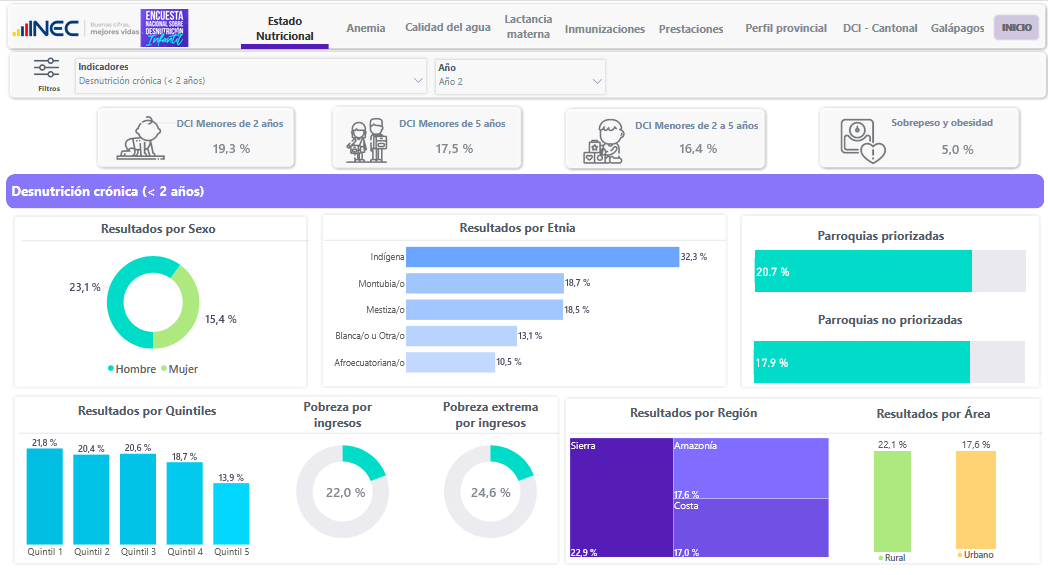
\includegraphics[width=0.85\textwidth]{figuras/inec-estado-nutricional.png}
  \caption{Panel de indicadores de desnutrición crónica en menores de 2 años. Fuente: INEC, ENSANUT 2018 \cite{inec2018ensanut}.}
  \label{fig:inec}
\end{figure}

\subsection{Nivel Micro}
Este trabajo no se desarrolló para una entidad receptora específica: es un prototipo académico de la Universidad Tecnológica Indoamérica que utiliza microdatos públicos de la ENSANUT 2018. La provincia de Tungurahua se toma como territorio de análisis por su combinación de áreas urbanas y rurales. En la base de modelado de este trabajo (niños de 0 a 59 meses; \num{18493} registros), \num{531} corresponden a Tungurahua, con una prevalencia muestral de \SI{30.9}{\percent} frente a \SI{24.7}{\percent} en el conjunto nacional de la misma base (Figura~\ref{fig:prevalencia}). Estas cifras son muestrales, no están ponderadas por el diseño de la encuesta y no son comparables con las estimaciones poblacionales del INEC, que corresponden a otra población de referencia (menores de dos años).

\begin{figure}[H]
  \centering
  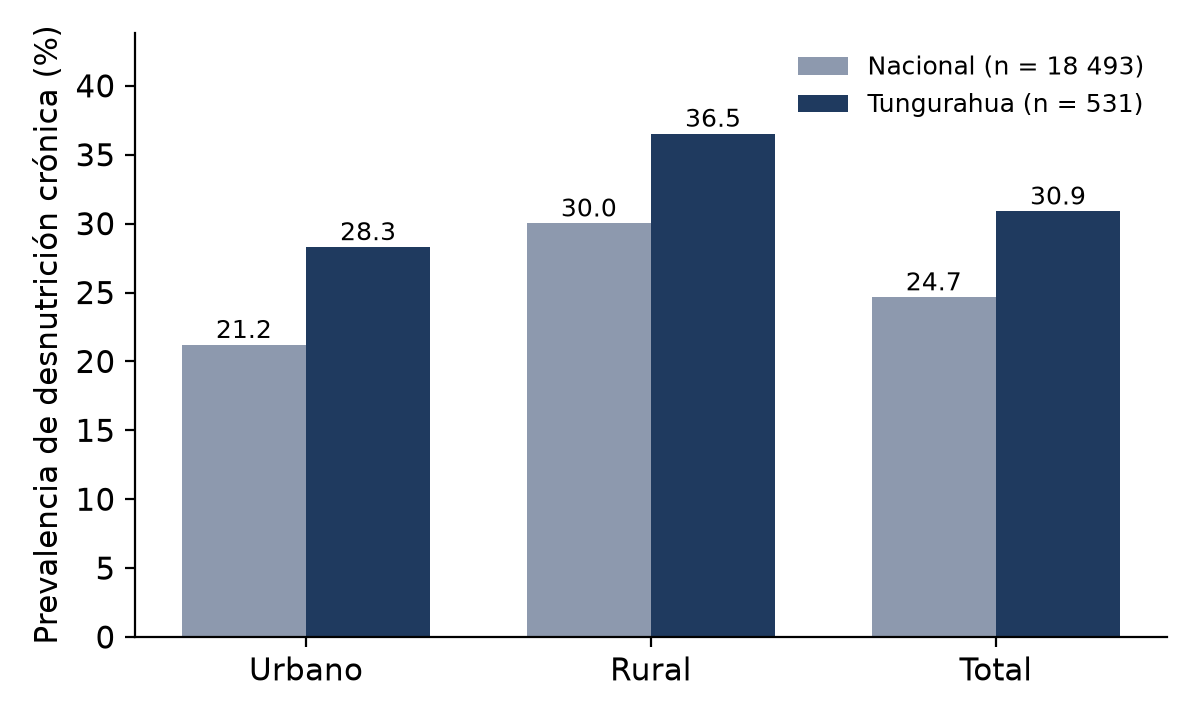
\includegraphics[width=0.75\textwidth]{figuras/prevalencia-area.png}
  \caption{Prevalencia muestral de desnutrición crónica por área de residencia: base nacional y subconjunto de Tungurahua. Elaboración propia a partir de la ENSANUT 2018 (sin ponderar).}
  \label{fig:prevalencia}
\end{figure}

\section{Estado del Arte}
\subsection{Protocolo de búsqueda}
La revisión se limitó a estudios que aplican ML a la clasificación del estado nutricional infantil o que describen el contexto nutricional de Ecuador. Se consultaron IEEE Xplore, ScienceDirect, MDPI, PubMed y Google Académico con combinaciones de los términos \textit{child malnutrition}, \textit{stunting}, \textit{machine learning}, \textit{ENSANUT} y \textit{Ecuador}. Se incluyeron artículos de 2019 a 2026 en español o inglés con texto completo disponible y se excluyeron los que no reportaban población, método o métricas. Se analizaron 10 trabajos, resumidos en la Tabla~\ref{tab:estado-arte}.

\begingroup
\footnotesize\setlength{\tabcolsep}{4pt}\arrayrulecolor{black!55}\renewcommand{\arraystretch}{1.15}
\begin{longtable}{|p{1.1cm}|p{2.7cm}|p{2.9cm}|p{2.7cm}|p{2.7cm}|}
  \caption{Comparación de los trabajos revisados con la presente tesis.}
  \label{tab:estado-arte}\\ \hline
  \enc{Estudio} & \enc{Datos y población} & \enc{Métodos y métricas} & \enc{Resultados y limitaciones} & \enc{Relación con la tesis}\\ \hline
  \endfirsthead
  \tablacont{5}\hline
  \enc{Estudio} & \enc{Datos y población} & \enc{Métodos y métricas} & \enc{Resultados y limitaciones} & \enc{Relación con la tesis}\\ \hline
  \endhead
  \hline\endfoot
  \cite{nu18142232} & ENDI 2023--2024 (Ecuador); \num{8344} niños de 0 a 23 meses; retraso en talla \SI{18.7}{\percent} & Modelos de ensamble con explicabilidad (SHAP); exactitud, ROC-AUC, precisión, F1, sensibilidad, especificidad y Brier en un conjunto de prueba & AUC de 0.62 a 0.66 (desempeño modesto a moderado); diseño transversal; SHAP no implica causalidad & Referente más cercano (mismo país e indicador). Sus AUC delimitan el rango esperable.\\ \hline
  \cite{ijerph22030449} & Metaanálisis de 11 estudios (de 789) con datos DHS; niños menores de 5 años & RF, gradient boosting, SVM, k-NN y regresión logística; riesgo de sesgo con PROBAST & Exactitud agrupada: \SI{68.92}{\percent} (talla), \SI{84.39}{\percent} (emaciación), \SI{73.60}{\percent} (bajo peso); $I^2$ = \SI{100}{\percent} & Da el nivel de referencia de exactitud y justifica reportar métricas por clase.\\ \hline
  \cite{Indrisari_Febiansyah_Adiwinoto_2025} & Revisión sistemática de 20 artículos (2020--2024) sobre retraso en talla en Indonesia & RF, SVM y redes neuronales; exactitud de \SI{72}{\percent} a \SI{99.92}{\percent} & Desbalance de clases, baja interpretabilidad y falta de validación externa & Justifica tratar el desbalance y declarar la ausencia de validación externa.\\ \hline
  \cite{11355002} & Revisión sistemática sobre predicción de retraso en talla (ODS 2 y 3) & Árboles de decisión, RF, redes neuronales y SVM & Resultados variables según calidad de los datos y metodología & Justifica comparar varios algoritmos con el mismo protocolo.\\ \hline
  \cite{11042152} & Estudio analítico de modelos; encuestas IDHS, BDHS y MICS & Árboles, SVM, RF, XGBoost y redes; comparación de metodologías & Falta de métricas estandarizadas y limitada generalización & Respalda la definición explícita de métricas y de partición.\\ \hline
  \cite{JANSSEN2024100264} & Revisión sistemática de IA en malnutrición (niños y adultos) & Predomina el aprendizaje supervisado & Más del \SI{90}{\percent} de los modelos no se usa en la práctica & Motiva declarar el alcance de prototipo académico.\\ \hline
  \cite{KIRK20222573} & Revisión sobre ML en investigación nutricional & Marco de trabajo; validación cruzada frente a partición simple & Riesgo de sobreajuste sin validación sólida & Sustenta la validación cruzada y el reporte del sobreajuste.\\ \hline
  \cite{ijerph23020240} & \num{303} recicladores de tres ciudades de Ecuador; adultos & RF, CatBoost y XGBoost; SMOTE solo en entrenamiento; ROC-AUC y sensibilidad por clase & Diseño transversal y tamaño muestral limitado & Ejemplo de manejo de desbalance sin fuga; población distinta.\\ \hline
  \cite{diagnostics16142147} & Datos demográficos del Hospital Isidro Ayora (Quito); preeclampsia & Seis modelos; F1 y SHAP; se añadió un conjunto sintético & F1 de 0.80 y AUC de 0.94 a 0.96; escasez de variables clínicas & Otro evento de salud en Ecuador; contexto del uso de ML con datos nacionales.\\ \hline
  \cite{nu17223608} & Revisión sistemática PRISMA de 17 estudios; cerca de \num{12000} niños ecuatorianos & Sin modelos de ML; síntesis de prevalencias y determinantes & Desnutrición crónica de \SI{15}{\percent} a \SI{35}{\percent}; mayor en zonas rurales e indígenas & Fundamenta las variables sociodemográficas y el contexto ecuatoriano.\\ \hline
\end{longtable}
\endgroup

\subsection{Criterios de selección y documentos excluidos}
La Tabla~\ref{tab:criterios} resume los criterios aplicados. La revisión se hizo sobre 15 documentos disponibles a texto completo; 10 cumplieron los criterios y se incluyeron en la Tabla~\ref{tab:estado-arte}. La Figura~\ref{fig:seleccion} muestra el flujo y la Tabla~\ref{tab:excluidos} los motivos de exclusión. No se registró el número de resultados devueltos por cada base de búsqueda, por lo que el flujo parte de los documentos ya reunidos y no constituye una revisión sistemática formal.

\begin{table}[H]
  \caption{Criterios de inclusión y exclusión.}
  \label{tab:criterios}
  \tablabase\small
  \begin{tabular}{|p{2.6cm}|p{5.6cm}|p{5.4cm}|}
    \hline
    \enc{Aspecto} & \enc{Inclusión} & \enc{Exclusión}\\ \hline
    Tema & Aplicación de ML a estado nutricional infantil, o contexto nutricional de Ecuador & Evaluación nutricional sin ML; temas ajenos a nutrición infantil\\ \hline
    Periodo & Publicaciones de 2019 a 2026 & Anteriores a 2019\\ \hline
    Idioma y acceso & Español o inglés; texto completo disponible & Sin texto completo\\ \hline
    Contenido mínimo & Población o fuente de datos, método y algún resultado o limitación & No reporta población, método o resultados\\ \hline
  \end{tabular}
\end{table}

\begin{figure}[H]
  \centering
  \begin{tikzpicture}[font=\footnotesize, node distance=6mm,
    caja/.style={draw=black!60, rounded corners=2pt, align=center, text width=4.4cm, minimum height=1.3cm, fill=white},
    flecha/.style={-{Stealth[length=2mm]}, black!60}]
    \node[caja] (a) {\textbf{Documentos reunidos}\\ 15 a texto completo};
    \node[caja, right=12mm of a] (b) {\textbf{Incluidos}\\ 10 en la Tabla~\ref{tab:estado-arte}};
    \node[caja, below=8mm of b] (c) {\textbf{Excluidos}\\ 5, con motivo en la Tabla~\ref{tab:excluidos}};
    \draw[flecha] (a) -- (b); \draw[flecha] (a.south) |- (c.west);
  \end{tikzpicture}
  \caption{Flujo de selección de los documentos revisados. Elaboración propia.}
  \label{fig:seleccion}
\end{figure}

\begin{table}[H]
  \caption{Documentos no incluidos en la comparación y motivo.}
  \label{tab:excluidos}
  \tablabase\small
  \begin{tabular}{|p{4.9cm}|p{8.7cm}|}
    \hline
    \enc{Documento} & \enc{Motivo de exclusión}\\ \hline
    Revisión narrativa sobre el modelo ABCDEFG de evaluación nutricional \cite{app16020845} & Evaluación nutricional clínica sin modelos de ML\\ \hline
    Comparación de métodos de evaluación nutricional del recién nacido \cite{nu17101642} & Neonatos y métodos antropométricos, sin ML\\ \hline
    Efecto de la austeridad sobre los niños en países de ingresos bajos y medios \cite{DAOUD2024102973} & Objetivo económico y de inferencia causal, no de clasificación nutricional\\ \hline
    Minería de datos y ML en diagnóstico clínico \cite{Saberi-Karimian19052021} & Enfoque clínico general, sin población infantil ni indicador nutricional\\ \hline
    Diagnóstico de malnutrición en preescolares con ML \cite{shindediagnosing} & Revisión sin población, métricas ni limitaciones comparables; se usa solo como contexto\\ \hline
  \end{tabular}
\end{table}


\subsection{Síntesis y aporte de la tesis}
Los trabajos revisados muestran tres patrones. Primero, los algoritmos de árboles y de \textit{boosting} son los más usados, pero ninguno es superior en todos los conjuntos de datos \cite{11355002}. Segundo, el desempeño reportado depende de la métrica: la exactitud puede ser alta o engañosa cuando las clases están desbalanceadas, y el estudio más reciente con datos ecuatorianos reporta AUC modestos de 0.62 a 0.66 \cite{nu18142232}. Tercero, la mayoría de los estudios usa validación interna, y la falta de validación externa y de interpretabilidad son limitaciones recurrentes \cite{Indrisari_Febiansyah_Adiwinoto_2025,JANSSEN2024100264}.

Frente a ello, esta tesis aporta: (i) un protocolo con prevención documentada de fuga de información y reporte de métricas por clase, incluida PR-AUC; (ii) una evaluación separada para Tungurahua con intervalos de confianza; y (iii) un prototipo reproducible (API y tablero) con casos de prueba funcionales. No aporta validación externa ni validación clínica.

\section{Planteamiento del Problema}
Los microdatos de la ENSANUT 2018 se emplean sobre todo para estimar prevalencias. Aprovecharlos con ML exige resolver tres dificultades verificables en la base: 350 variables en \num{20510} registros con códigos numéricos y valores especiales; \num{2017} registros (\SI{9.8}{\percent}) sin la variable objetivo; y desbalance de clases cercano a 3 a 1. A esto se suma la escasa evidencia, para Tungurahua, de cuánto funciona un clasificador entrenado con datos nacionales. El problema central es, por tanto, la ausencia de un procedimiento reproducible que clasifique la desnutrición crónica infantil con métricas por clase y muestre su desempeño para Tungurahua (Figura~\ref{fig:arbol}).

\begin{figure}[H]
  \centering
  \begin{tikzpicture}[font=\footnotesize, node distance=6mm,
    caja/.style={draw=black!60, rounded corners=2pt, align=center, text width=4.1cm, inner sep=4pt, fill=white},
    central/.style={draw=black!80, thick, rounded corners=2pt, align=center, text width=11cm, inner sep=6pt, fill=black!6},
    flecha/.style={-{Stealth[length=2mm]}, black!60}]
    \node[caja] (e1) {Conclusiones basadas en exactitud global, poco informativa con clases desbalanceadas};
    \node[caja, right=3mm of e1] (e2) {Análisis manual, difícil de reproducir};
    \node[caja, right=3mm of e2] (e3) {Sin evidencia de desempeño para Tungurahua};
    \node[central, below=10mm of e2] (c) {\textbf{PROBLEMA CENTRAL}\\ Ausencia de un procedimiento reproducible que clasifique la desnutrición crónica infantil con métricas por clase y evalúe su desempeño en Tungurahua};
    \node[caja, below=10mm of c] (c2) {Datos fragmentados: 350 variables, valores especiales y códigos numéricos};
    \node[caja, left=3mm of c2] (c1) {\num{2017} registros (\SI{9.8}{\percent}) sin variable objetivo};
    \node[caja, right=3mm of c2] (c3) {Desbalance de clases (\SI{24.7}{\percent} de casos) y pocos registros de Tungurahua (531)};
    \foreach \n in {e1,e2,e3} \draw[flecha] (c.north) -- (\n.south);
    \foreach \n in {c1,c2,c3} \draw[flecha] (\n.north) -- (c.south);
    \node[above=1mm of e2, font=\footnotesize\bfseries] {EFECTOS};
    \node[below=1mm of c2, font=\footnotesize\bfseries] {CAUSAS};
  \end{tikzpicture}
  \caption{Árbol de problemas: causas y efectos identificados en la base ENSANUT 2018. Elaboración propia.}
  \label{fig:arbol}
\end{figure}

\section{Justificación}
La desnutrición crónica es un indicador prioritario de salud pública y sus datos oficiales rara vez se explotan con modelos de clasificación evaluados de forma transparente. Documentar un procedimiento completo, con sus resultados modestos y sus límites, aporta evidencia útil para futuros estudios con datos ecuatorianos, en un contexto en que los propios trabajos recientes reportan AUC de 0.62 a 0.66 \cite{nu18142232}.

El proyecto es factible porque usa microdatos públicos ya recolectados, por lo que no requiere trabajo de campo. Las herramientas empleadas son de código abierto: Python y scikit-learn para el modelado, FastAPI para el servicio web y React para el tablero. El desarrollo se ejecutó en un equipo personal, sin costos de licencias.

Como aporte técnico, el trabajo integra en un mismo flujo la preparación de datos, la comparación de cuatro algoritmos, la selección del umbral de decisión, un servicio REST con validación de entradas y un tablero de consulta. Todo se entrega como herramienta exploratoria de apoyo analítico; no es un sistema de diagnóstico clínico ni una solución validada para decisiones médicas.

Los beneficiarios directos son estudiantes e investigadores que necesiten un procedimiento reproducible para clasificar la condición nutricional con datos de la ENSANUT. Indirectamente, el trabajo puede servir de base para estudios de vigilancia nutricional en Tungurahua, siempre que se complemente con validación externa.

El trabajo se alinea con el ODS 2 (Hambre cero) por su foco en la desnutrición infantil, con el ODS 3 (Salud y bienestar) por su relación con la salud en la primera infancia y con el ODS 9 (Industria, innovación e infraestructura) por la construcción de una solución digital reproducible.

\section{Objetivos}
\subsection{Objetivo General}
Desarrollar y evaluar, como prototipo académico, un clasificador de desnutrición crónica infantil basado en Machine Learning, aplicando la metodología OSEMN a los microdatos de la ENSANUT 2018 y exponiéndolo mediante una API REST y un tablero web, con evaluación específica para Tungurahua.

\subsection{Objetivos Específicos}
\begin{itemize}
  \item Analizar y preparar los microdatos de la ENSANUT 2018, verificando la calidad de los datos, la definición de la variable objetivo y la ausencia de fuga de información.
  \item Diseñar la arquitectura de la solución y el protocolo experimental (partición, preprocesamiento, métricas por clase y criterio de selección).
  \item Entrenar y comparar cuatro algoritmos de clasificación y evaluar el modelo seleccionado en el conjunto de prueba nacional y en el subconjunto de Tungurahua.
  \item Implementar una API REST y un tablero web que permitan consultar predicciones, métricas e indicadores.
  \item Validar el funcionamiento de la API mediante casos de prueba y documentar las limitaciones del prototipo.
\end{itemize}

\section{Alcance del Proyecto}
El estudio trabaja con la variable objetivo \textit{desnutrición crónica} (binaria) en niños de 0 a 59 meses de la ENSANUT 2018. El modelo se entrena con los registros de todo el país que tienen la variable medida y se evalúa por separado para Tungurahua. El diseño es transversal, por lo que el modelo \emph{clasifica} la condición observada al momento de la encuesta; no anticipa casos futuros. La Tabla~\ref{tab:alcance} resume lo que incluye y excluye.

\begin{table}[H]
  \caption{Alcance y exclusiones del proyecto.}
  \label{tab:alcance}
  \tablabase\small
  \begin{tabular}{|p{6.5cm}|p{7.0cm}|}
    \hline
    \enc{Incluye} & \enc{Excluye}\\ \hline
    Microdatos ENSANUT 2018, módulo de salud de la niñez (0 a 59 meses); 114 predictores. & Otras encuestas en el modelo. La ENDI se exploró, pero no alimenta el entrenamiento ni la evaluación.\\ \hline
    Comparación de regresión logística, árbol de decisión, Random Forest y XGBoost. & Aprendizaje profundo y modelos híbridos.\\ \hline
    Evaluación con métricas por clase en el conjunto de prueba nacional y en Tungurahua. & Resultados por cantón o parroquia, y validación externa o clínica.\\ \hline
    API REST y tablero web de consulta, desplegados como prototipo. & Autenticación, base de datos, historias clínicas y datos en tiempo real.\\ \hline
    Documentación técnica, manual de uso y casos de prueba. & Uso como herramienta de diagnóstico o de decisión médica.\\ \hline
  \end{tabular}
\end{table}

\section{Fundamentación Teórica}
\subsection{Desnutrición crónica}
La desnutrición crónica es el retraso del crecimiento en talla para la edad, asociado a deficiencias nutricionales prolongadas. Se distingue de la emaciación (bajo peso para la talla) y del bajo peso (bajo peso para la edad), que son otras formas de malnutrición \cite{11042152}. En este trabajo se usa el indicador binario incluido en la base de la ENSANUT (1 = con desnutrición crónica; 0 = sin desnutrición crónica), y no se emplea como sinónimo de malnutrición ni de estado nutricional en general.

\subsection{Clasificación con datos transversales}
Una encuesta transversal mide a cada niño una sola vez. Con esos datos un modelo estima la probabilidad de una condición ya presente a partir de sus características, pero no puede anticipar eventos futuros. Por eso este trabajo emplea los términos \emph{clasificar} y \emph{estimar la condición observada}.

\subsection{Desbalance de clases y umbral de decisión}
Cuando la clase de interés es minoritaria, un modelo puede alcanzar exactitud alta ignorándola. Se recomienda ponderar las clases o remuestrear y evaluar con métricas por clase \cite{he2009learning}. El umbral de probabilidad de \num{0.5} favorece a la clase mayoritaria, por lo que puede ajustarse según el objetivo de la aplicación \cite{provost2000machine}.

\subsection{Fuga de información y validación}
Hay fuga de información cuando el entrenamiento usa datos que revelan la variable objetivo o información de la partición de prueba \cite{kaufman2011leakage}. Se previene ajustando imputación y escalado solo con la partición de entrenamiento, y verificando que ningún predictor sea una versión de la variable objetivo. La validación cruzada estratificada permite ajustar hiperparámetros sin usar la partición de prueba \cite{refaeilzadeh2009cross}.

\subsection{Métricas de evaluación}
Se usan la sensibilidad, la especificidad, la precisión, el F1 de la clase positiva, la exactitud balanceada, el ROC-AUC \cite{fawcett2006introduction} y el PR-AUC. Con clases desbalanceadas, el PR-AUC es más informativo que la exactitud porque no depende de los verdaderos negativos.

\subsection{Algoritmos comparados}
La regresión logística y el árbol de decisión son modelos base. Random Forest promedia muchos árboles entrenados con muestras aleatorias \cite{breiman2001random}, y XGBoost construye árboles de forma secuencial para corregir errores previos \cite{chen2016xgboost}. Los cuatro se eligieron por su uso frecuente en la literatura revisada (Tabla~\ref{tab:estado-arte}).

\subsection{Interpretabilidad, privacidad y sesgo}
La importancia de variables de un bosque aleatorio describe cuánto usa el modelo cada variable, pero no implica causalidad. Los microdatos de la ENSANUT son públicos y no incluyen identificadores personales directos. Existe sesgo de representatividad cuando un territorio aporta pocos registros: en Tungurahua se dispone de \num{531}, lo que limita la precisión de las estimaciones locales.

\subsection{API REST y tablero web}
Una API REST expone funciones del modelo mediante peticiones HTTP. FastAPI es una biblioteca de Python que valida los datos de entrada con anotaciones de tipo y genera documentación interactiva \cite{ramirez2022deploying}. El tablero es una aplicación web en React que consume la API.

\subsection{Metodología OSEMN}
OSEMN organiza un proyecto de ciencia de datos en cinco fases: obtener (\textit{Obtain}), limpiar (\textit{Scrub}), explorar (\textit{Explore}), modelar (\textit{Model}) e interpretar (\textit{iNterpret}). En este trabajo se usa como guía para ordenar y documentar las actividades, no como garantía de calidad de los resultados.

\chapter{Metodología}

\section{Diagnóstico de la Situación Actual}
Este diagnóstico describe cómo se aprovechan hoy los microdatos de la ENSANUT 2018 y qué características de los datos condicionan el desarrollo. El proceso actual se reconstruyó a partir de la documentación oficial de la encuesta y del trabajo previo de exploración del autor; no se midieron tiempos de ejecución ni se entrevistó a usuarios, por lo que esos aspectos se declaran como limitación.

\subsection{Proceso actual (AS-IS)}
La Tabla~\ref{tab:asis} resume los elementos del proceso y la Figura~\ref{fig:asis} su flujo.

\begin{table}[H]
  \caption{Proceso actual de aprovechamiento de los microdatos de la ENSANUT 2018.}
  \label{tab:asis}
  \tablabase\small
  \begin{tabular}{|p{3.0cm}|p{10.6cm}|}
    \hline
    \enc{Elemento} & \enc{Descripción}\\ \hline
    Usuarios & Investigadores, estudiantes y analistas que consultan la ENSANUT.\\ \hline
    Fuentes & Microdatos públicos del INEC (módulo de salud de la niñez), diccionario de datos y metadatos de la encuesta.\\ \hline
    Herramientas & Tablas y paneles publicados por el INEC; para análisis propios, hojas de cálculo o software estadístico. No se identificó una herramienta específica en la UTI.\\ \hline
    Salidas & Prevalencias por grupo (área, etnia, quintil de ingresos). No hay clasificación individual ni métricas por clase.\\ \hline
    Responsables & INEC (publicación); el analista (procesamiento e interpretación).\\ \hline
    Limitaciones & Códigos numéricos que requieren el diccionario; \num{2017} registros sin variable objetivo; desbalance de clases; procesamiento manual difícil de reproducir.\\ \hline
  \end{tabular}
\end{table}

\begin{figure}[H]
  \centering
  \begin{tikzpicture}[font=\footnotesize, node distance=5mm,
    caja/.style={draw=black!60, rounded corners=2pt, align=center, text width=3.0cm, minimum height=1.3cm, fill=white},
    flecha/.style={-{Stealth[length=2mm]}, black!60}]
    \node[caja] (a) {El INEC publica microdatos y diccionario};
    \node[caja, right=of a] (b) {Descarga y codificación manual};
    \node[caja, right=of b] (c) {Análisis descriptivo (prevalencias)};
    \node[caja, right=of c] (d) {Informe o panel de indicadores};
    \draw[flecha] (a) -- (b); \draw[flecha] (b) -- (c); \draw[flecha] (c) -- (d);
  \end{tikzpicture}
  \caption{Flujo actual (AS-IS) de aprovechamiento de los microdatos de la ENSANUT. Elaboración propia.}
  \label{fig:asis}
\end{figure}

\subsection{Hallazgos sobre los datos}
La exploración inicial de la base produjo los resultados de la Tabla~\ref{tab:datos}. El hallazgo con mayor efecto metodológico fue que el \SI{9.8}{\percent} de los registros no tenía medida la variable objetivo.

\begin{table}[H]
  \caption{Características de la base de datos.}
  \label{tab:datos}
  \tablabase\small
  \begin{tabular}{|p{8.2cm}|r|}
    \hline
    \enc{Característica} & \enc{Valor}\\ \hline
    Registros originales (módulo de salud de la niñez) & \num{20510}\\ \hline
    Variables originales & 350\\ \hline
    Registros sin variable objetivo medida & \num{2017} (\SI{9.8}{\percent})\\ \hline
    Registros del modelo (con variable objetivo) & \num{18493}\\ \hline
    Predictores del modelo & 114\\ \hline
    Casos con desnutrición crónica (clase 1) & \num{4560} (\SI{24.7}{\percent})\\ \hline
    Casos sin desnutrición crónica (clase 0) & \num{13933} (\SI{75.3}{\percent})\\ \hline
    Rango de edad & 0 a 59 meses\\ \hline
    Registros de Tungurahua con variable objetivo & 531 (164 casos; \SI{30.9}{\percent})\\ \hline
    Predictores con valores ausentes en la base original & 84 de 114 (32 con más del \SI{10}{\percent})\\ \hline
  \end{tabular}
\end{table}

\subsection{Síntesis del diagnóstico}
Del diagnóstico se derivan tres necesidades: (i) un procedimiento de preparación reproducible que excluya, y no imponga, la variable objetivo faltante; (ii) una evaluación con métricas por clase que considere el desbalance; y (iii) un medio de consulta (API y tablero) que permita usar el modelo y revisar su desempeño. Estas necesidades sustentan los requerimientos de la sección correspondiente.

\section{Metodología de Desarrollo o Implementación}
\subsection{Enfoque de investigación}
La investigación es aplicada, cuantitativa, no experimental y transversal, porque usa datos secundarios de una sola medición para construir y evaluar un clasificador. El nivel de análisis es de clasificación con componente correlacional; no se buscan relaciones causales.

\subsection{Metodología OSEMN}
OSEMN se ejecutó como proceso de cinco fases (Figura~\ref{fig:osemn}). La Tabla~\ref{tab:osemn} indica, para cada fase, sus entradas, actividades, decisiones, salidas y evidencia. Los scripts y notebooks citados están en el repositorio del proyecto (Anexo~E).

\begin{figure}[H]
  \centering
  \begin{tikzpicture}[font=\footnotesize, node distance=4mm,
    caja/.style={draw=black!60, rounded corners=2pt, align=center, text width=2.3cm, minimum height=1.6cm, fill=white},
    flecha/.style={-{Stealth[length=2mm]}, black!60}]
    \node[caja] (o) {\textbf{Obtener}\\ ENSANUT 2018 (CSV)};
    \node[caja, right=of o] (s) {\textbf{Limpiar}\\ Base de \num{18493} registros};
    \node[caja, right=of s] (e) {\textbf{Explorar}\\ Perfil y control de fuga};
    \node[caja, right=of e] (m) {\textbf{Modelar}\\ Comparación y selección};
    \node[caja, right=of m] (n) {\textbf{Interpretar}\\ Métricas, API y tablero};
    \foreach \a/\b in {o/s,s/e,e/m,m/n} \draw[flecha] (\a) -- (\b);
  \end{tikzpicture}
  \caption{Fases de la metodología OSEMN aplicadas en el proyecto. Elaboración propia.}
  \label{fig:osemn}
\end{figure}

\begingroup
\scriptsize\setlength{\tabcolsep}{3pt}\arrayrulecolor{black!55}\renewcommand{\arraystretch}{1.15}
\begin{longtable}{|p{1.3cm}|p{2.0cm}|p{3.4cm}|p{2.6cm}|p{2.2cm}|p{1.9cm}|}
  \caption{Fases de OSEMN ejecutadas: entradas, actividades, decisiones, salidas y evidencia.}
  \label{tab:osemn}\\ \hline
  \enc{Fase} & \enc{Entradas} & \enc{Actividades} & \enc{Decisiones} & \enc{Salidas} & \enc{Evidencia}\\ \hline
  \endfirsthead
  \tablacont{6}\hline
  \enc{Fase} & \enc{Entradas} & \enc{Actividades} & \enc{Decisiones} & \enc{Salidas} & \enc{Evidencia}\\ \hline
  \endhead
  \hline\endfoot
  Obtener & Microdatos ENSANUT 2018; diccionario y metadatos & Carga del CSV; revisión de estructura y de tipos & Usar solo ENSANUT en el modelo; ENDI solo exploratoria & Base bruta: \num{20510} $\times$ 350 & Notebook de limpieza\\ \hline
  Limpiar & Base bruta & Renombrar variables; convertir valores especiales en nulos; eliminar registros sin variable objetivo; definir 114 predictores & Excluir (no imputar) la variable objetivo faltante & Base del modelo: \num{18493} $\times$ 115 & Script de limpieza\\ \hline
  Explorar & Base del modelo & Distribuciones y prevalencias; comparación Tungurahua y nacional; revisión de fuga por variable & Mantener variables sin señal de fuga (AUC univariado $<$ 0.95) & Perfil de datos; lista de limitaciones & Script de revisión de fuga; notebook EDA\\ \hline
  Modelar & Base del modelo & Partición 80/20 estratificada (semilla 42); preprocesamiento en \textit{Pipeline}; 4 algoritmos con manejo de desbalance; búsqueda de hiperparámetros con validación cruzada; ajuste del umbral & Selección por PR-AUC; umbral que maximiza F1 de la clase 1 (validación cruzada en entrenamiento) & \texttt{modelo\_v2.joblib}; \texttt{metricas\_v2.json} & Script de entrenamiento\\ \hline
  Interpretar & Modelo y particiones & Métricas por clase con intervalos; importancia de variables; API y tablero; pruebas funcionales & Reportar sobreajuste y límites & Resultados (cap. III) y prototipo & Anexos A, C y D\\ \hline
\end{longtable}
\endgroup

\subsection{Protocolo experimental}
La base del modelo se dividió en \num{14794} registros de entrenamiento y \num{3699} de prueba (partición 80/20 estratificada por la variable objetivo, semilla 42). El preprocesamiento se encapsuló en un \textit{Pipeline} de scikit-learn \cite{pedregosa2011scikit}: variables numéricas con imputación por mediana y estandarización, y variables categóricas con imputación por moda y codificación \textit{one-hot}. La estandarización y la codificación se ajustan solo con los datos de entrenamiento. La imputación del \textit{Pipeline}, en cambio, no tiene efecto porque la base del modelo ya no contiene nulos: los faltantes se imputaron antes de la partición (Tabla~\ref{tab:reglas}).

Para el desbalance se usó ponderación de clases (\texttt{class\_weight="balanced"} en los modelos que la admiten y \texttt{scale\_pos\_weight} en XGBoost). Los hiperparámetros del modelo seleccionado se buscaron con búsqueda aleatoria \cite{bergstra2012random} y validación cruzada estratificada de 5 particiones sobre el entrenamiento, con PR-AUC como criterio. El umbral de decisión se eligió como el valor que maximiza el F1 de la clase positiva con predicciones de validación cruzada sobre el entrenamiento. La comparación de los cuatro modelos base se calculó sobre la partición de prueba, lo que puede hacer levemente optimista el PR-AUC reportado; esta limitación se retoma en el Capítulo~III.

\subsection{Reglas de limpieza y preparación}
La Tabla~\ref{tab:reglas} detalla las reglas aplicadas al construir la base del modelo. El código correspondiente está en el Anexo~I.

\begin{table}[H]
  \caption{Reglas de limpieza y preparación de la base.}
  \label{tab:reglas}
  \tablabase\footnotesize
  \begin{tabular}{|c|p{5.0cm}|p{6.9cm}|}
    \hline
    \enc{N.º} & \enc{Regla} & \enc{Justificación y verificación}\\ \hline
    1 & Excluir los registros con variable objetivo sin medir & Se evita fabricar etiquetas. Se excluyeron \num{2017} registros y quedaron \num{18493}\\ \hline
    2 & Alinear la base cruda y la base renombrada por posición & Se verificó que las etiquetas de los \num{18493} registros medidos coinciden al \SI{100}{\percent}; si difiere, el script se detiene\\ \hline
    3 & Convertir valores especiales en nulos & Unifica códigos de no respuesta antes de imputar\\ \hline
    4 & Imputación de valores ausentes & La base del modelo no tiene nulos: se imputaron con mediana o moda en la limpieza inicial, sobre todos los registros y antes de la partición (limitación; Capítulo~III). El imputador del \textit{Pipeline} queda sin efecto\\ \hline
    5 & Separar entrenamiento y prueba antes del modelado & Partición 80/20 estratificada con semilla 42\\ \hline
    6 & Revisar fuga por variable & AUC univariado $\leq$ 0.95 en todas las variables evaluadas\\ \hline
    7 & Exigir que toda columna sea numérica o categórica & Una prueba detiene el proceso si alguna columna quedara fuera del modelo\\ \hline
  \end{tabular}
\end{table}

\subsection{Búsqueda de hiperparámetros}
Solo el algoritmo ganador recibió búsqueda de hiperparámetros. Para Random Forest se muestrearon 40 combinaciones (\textit{RandomizedSearchCV}) con validación cruzada estratificada de 5 particiones y PR-AUC como criterio (Tabla~\ref{tab:grilla}). Se acotó la profundidad y el tamaño de las hojas para reducir el tamaño del modelo (de 170 MB a 28 MB) y el sobreajuste.

\begin{table}[H]
  \caption{Espacio de búsqueda de Random Forest y valores seleccionados.}
  \label{tab:grilla}
  \tablabase\small
  \begin{tabular}{|p{4.6cm}|p{5.6cm}|c|}
    \hline
    \enc{Hiperparámetro} & \enc{Valores explorados} & \enc{Seleccionado}\\ \hline
    \texttt{n\_estimators} & 100, 150, 200, 300 & 300\\ \hline
    \texttt{max\_depth} & 5, 8, 10, 15, 20 & 20\\ \hline
    \texttt{min\_samples\_leaf} & 1, 2, 5, 10 & 10\\ \hline
    \texttt{min\_samples\_split} & 2, 5, 10 & 2\\ \hline
    \texttt{max\_features} & \texttt{sqrt}, \texttt{log2} & \texttt{sqrt}\\ \hline
  \end{tabular}
\end{table}

\subsection{Riesgos del proyecto y mitigación}
\begin{table}[H]
  \caption{Riesgos identificados y medidas aplicadas.}
  \label{tab:riesgos}
  \tablabase\footnotesize
  \begin{tabular}{|p{3.3cm}|p{4.9cm}|p{5.4cm}|}
    \hline
    \enc{Riesgo} & \enc{Efecto posible} & \enc{Medida en el proyecto}\\ \hline
    Fuga de información & Métricas infladas & Exclusión de la variable objetivo faltante, \textit{Pipeline} y revisión univariada; persiste la imputación previa a la partición\\ \hline
    Desbalance de clases & Modelo que ignora la clase 1 & Ponderación de clases, umbral ajustado y métricas por clase\\ \hline
    Sobreajuste & Desempeño real menor al de entrenamiento & Regularización y reporte de la brecha entrenamiento--prueba\\ \hline
    Representatividad territorial & Estimaciones imprecisas para Tungurahua & Intervalos de confianza y advertencia de uso\\ \hline
    Uso indebido como diagnóstico & Decisiones clínicas sin sustento & Aviso de herramienta académica y alcance declarado\\ \hline
    Acceso no autorizado a la API & Uso o abuso del servicio & Pendiente: no hay autenticación (Capítulo~III)\\ \hline
  \end{tabular}
\end{table}



\subsection{Métricas de evaluación}
Con VP, VN, FP y FN los verdaderos positivos, verdaderos negativos, falsos positivos y falsos negativos de la clase 1 (con desnutrición crónica), se calcularon:
\begin{equation}
  \text{Sensibilidad} = \frac{VP}{VP + FN}
  \eqindice{Sensibilidad (recall)}
\end{equation}
\begin{equation}
  \text{Especificidad} = \frac{VN}{VN + FP}
  \eqindice{Especificidad}
\end{equation}
\begin{equation}
  \text{Precisión} = \frac{VP}{VP + FP}
  \eqindice{Precisión}
\end{equation}
\begin{equation}
  F_1 = 2\,\frac{\text{Precisión}\times\text{Sensibilidad}}{\text{Precisión}+\text{Sensibilidad}}
  \eqindice{F1 de la clase positiva}
\end{equation}
\begin{equation}
  \text{Exactitud balanceada} = \frac{\text{Sensibilidad} + \text{Especificidad}}{2}
  \eqindice{Exactitud balanceada}
\end{equation}
Además se reportan el ROC-AUC y el PR-AUC. La clase prioritaria es la 1 (niños con desnutrición crónica) porque omitirla (falso negativo) es el error más costoso en una aplicación de tamizaje; por eso se prioriza la sensibilidad, aceptando una precisión menor.

\section{Técnicas e Instrumentos de Recolección de Información}
La Tabla~\ref{tab:tecnicas} lista las técnicas realmente aplicadas. No se realizaron entrevistas, encuestas ni validación con expertos, por lo que no se presentan resultados de ese tipo.

\begin{table}[H]
  \caption{Técnicas e instrumentos aplicados.}
  \label{tab:tecnicas}
  \tablabase\small
  \begin{tabular}{|p{3.2cm}|p{5.7cm}|p{4.1cm}|}
    \hline
    \enc{Técnica} & \enc{Instrumento} & \enc{Uso en el proyecto}\\ \hline
    Revisión documental & Artículos indexados (IEEE Xplore, ScienceDirect, MDPI, PubMed) según el protocolo del Capítulo~I & Estado del arte y elección de algoritmos\\ \hline
    Análisis de microdatos & Base ENSANUT 2018 (CSV), diccionario y metadatos; \textit{pandas} & Caracterización y limpieza\\ \hline
    Experimentación computacional & Notebooks y scripts en Python; scikit-learn y XGBoost & Entrenamiento y comparación de modelos\\ \hline
    Pruebas funcionales & Casos de prueba sobre la API (\textit{TestClient} de FastAPI) y pruebas automáticas con \textit{pytest} & Verificación del servicio (Anexo~C)\\ \hline
  \end{tabular}
\end{table}

\section{Requerimientos del Proyecto}
Los requerimientos se formularon de modo que cada uno tenga un criterio de aceptación comprobable. Su cumplimiento se verifica en el Capítulo~III.

\subsection{Requerimientos Funcionales}
\begin{table}[H]
  \caption{Requerimientos funcionales y criterios de aceptación.}
  \label{tab:rf}
  \tablabase\footnotesize
  \begin{tabular}{|c|p{4.1cm}|p{6.6cm}|c|}
    \hline
    \enc{ID} & \enc{Requerimiento} & \enc{Criterio de aceptación} & \enc{Prioridad}\\ \hline
    RF1 & Preprocesamiento reproducible & Imputación y escalado ajustados solo con el entrenamiento; resultados idénticos con semilla 42. & Alta\\ \hline
    RF2 & Comparación de modelos & Cuatro algoritmos evaluados con la misma partición y reporte de sensibilidad, especificidad, precisión, F1, exactitud balanceada, ROC-AUC y PR-AUC. & Alta\\ \hline
    RF3 & Predicción individual & \texttt{POST /predict} con las 114 variables devuelve clase, probabilidad y nivel de riesgo; responde HTTP 400 si las variables no coinciden. & Alta\\ \hline
    RF4 & Predicción masiva & \texttt{POST /predict-file} recibe un archivo y devuelve un \texttt{.xlsx} con una fila por registro. & Media\\ \hline
    RF5 & Consulta de métricas & \texttt{GET /dashboard/metricas} devuelve las métricas del archivo \texttt{metricas\_v2.json}. & Alta\\ \hline
    RF6 & Indicadores del tablero & \texttt{GET /dashboard} admite filtro por provincia; \texttt{GET /dashboard/importancia} lista la importancia de variables. & Media\\ \hline
    RF7 & Documentación interactiva & \texttt{GET /docs} muestra la documentación OpenAPI. & Media\\ \hline
    RF8 & Selección de versión del modelo & La variable de entorno \texttt{MODEL\_VERSION} (v1 o v2) define el modelo activo; por defecto v2. & Baja\\ \hline
  \end{tabular}
\end{table}

\subsection{Requerimientos No Funcionales}
\begin{table}[H]
  \caption{Requerimientos no funcionales y criterios de aceptación.}
  \label{tab:rnf}
  \tablabase\footnotesize
  \begin{tabular}{|c|p{2.6cm}|p{7.5cm}|c|}
    \hline
    \enc{ID} & \enc{Atributo} & \enc{Criterio de aceptación} & \enc{Prioridad}\\ \hline
    RNF1 & Validación de entradas & El \SI{100}{\percent} de las solicitudes con variables faltantes o sobrantes se rechaza con HTTP 400. & Alta\\ \hline
    RNF2 & Rendimiento & Latencia mediana de \texttt{POST /predict} $\leq$ 200 ms, medida sobre 100 solicitudes. & Media\\ \hline
    RNF3 & Disponibilidad & \texttt{GET /health} responde HTTP 200 mientras el servicio esté desplegado. & Media\\ \hline
    RNF4 & Seguridad y acceso & Autenticación y control de acceso a la API (no implementada por decisión de alcance; Capítulo~III). & Media\\ \hline
    RNF5 & Reproducibilidad & Semilla fija (42) y versiones de librerías fijadas en \texttt{requirements.txt}. & Alta\\ \hline
    RNF6 & Mantenibilidad & Código separado por módulos y al menos 5 pruebas automáticas aprobadas. & Media\\ \hline
    RNF7 & Uso responsable & La interfaz y los documentos indican que es una herramienta académica exploratoria y no un sistema de diagnóstico. & Alta\\ \hline
  \end{tabular}
\end{table}

\section{Diseño de la Solución}
\subsection{Arquitectura y flujo de datos}
La solución tiene cuatro componentes (Figura~\ref{fig:arquitectura}): (1) el pipeline de datos y modelado, que produce (2) los artefactos del modelo (\texttt{modelo\_v2.joblib} y \texttt{metricas\_v2.json}); (3) la API REST, que carga los artefactos y expone los servicios; y (4) el tablero web, que consume la API. La Figura~\ref{fig:flujo-pred} muestra el flujo de una predicción individual.

\begin{figure}[H]
  \centering
  \begin{tikzpicture}[font=\footnotesize, node distance=6mm,
    caja/.style={draw=black!60, rounded corners=2pt, align=center, text width=3.5cm, minimum height=1.5cm, fill=white},
    flecha/.style={-{Stealth[length=2mm]}, black!60}]
    \node[caja] (d) {\textbf{Datos}\\ ENSANUT 2018 (CSV)};
    \node[caja, right=of d] (p) {\textbf{1. Pipeline de datos y modelado}\\ Python, scikit-learn};
    \node[caja, right=of p] (a) {\textbf{2. Artefactos}\\ \texttt{modelo\_v2.joblib}\\ \texttt{metricas\_v2.json}};
    \node[caja, below=8mm of a] (api) {\textbf{3. API REST}\\ FastAPI};
    \node[caja, left=of api] (w) {\textbf{4. Tablero web}\\ React};
    \node[caja, left=of w] (u) {\textbf{Usuario}\\ navegador o cliente HTTP};
    \draw[flecha] (d) -- (p); \draw[flecha] (p) -- (a); \draw[flecha] (a) -- (api);
    \draw[flecha] (api) -- (w); \draw[flecha] (w) -- (u);
  \end{tikzpicture}
  \caption{Arquitectura y flujo de datos de la solución. Elaboración propia.}
  \label{fig:arquitectura}
\end{figure}

\begin{figure}[H]
  \centering
  \begin{tikzpicture}[font=\footnotesize, node distance=4mm,
    caja/.style={draw=black!60, rounded corners=2pt, align=center, text width=2.2cm, minimum height=1.5cm, fill=white},
    flecha/.style={-{Stealth[length=2mm]}, black!60}]
    \node[caja] (c) {Cliente envía JSON con 114 variables};
    \node[caja, right=of c] (v) {Validación: nombres y cantidad};
    \node[caja, right=of v] (m) {Pipeline: preprocesador y Random Forest};
    \node[caja, right=of m] (u) {Probabilidad y umbral 0.42};
    \node[caja, right=of u] (r) {Respuesta: clase, probabilidad y riesgo};
    \foreach \a/\b in {c/v,v/m,m/u,u/r} \draw[flecha] (\a) -- (\b);
    \node[draw=black!60, rounded corners=2pt, align=center, text width=2.5cm, below=6mm of v, font=\scriptsize] (e) {HTTP 400 si no coinciden};
    \draw[flecha] (v) -- (e);
  \end{tikzpicture}
  \caption{Flujo de una predicción individual (\texttt{POST /predict}). Elaboración propia.}
  \label{fig:flujo-pred}
\end{figure}

\subsection{Modelo de datos}
El modelo usa 114 predictores de la ENSANUT agrupados en nueve bloques (Tabla~\ref{tab:vars}); el listado completo está en el Anexo~F. La variable objetivo es \texttt{desnutricion\_cronica}. No se incluyen la talla ni el peso actuales del niño; sí se incluyen dos variables de diseño muestral (\texttt{factor\_expansion} y \texttt{estrato}), que se discuten como limitación en el Capítulo~III.

\begin{table}[H]
  \caption{Grupos de variables predictoras.}
  \label{tab:vars}
  \tablabase\footnotesize
  \begin{tabular}{|p{4.6cm}|c|p{6.4cm}|}
    \hline
    \enc{Grupo} & \enc{N.º} & \enc{Ejemplos}\\ \hline
    Territorio y demografía & 10 & provincia, área, sexo, edad en meses, etnia y educación de la madre, estrato\\ \hline
    Orden del hijo & 1 & orden del hijo\\ \hline
    Embarazo y control prenatal & 25 & controles prenatales, micronutrientes, exámenes, consejería\\ \hline
    Parto y recién nacido & 19 & tipo de parto, prematuridad, peso y talla al nacer\\ \hline
    Control posparto & 3 & control posparto y lugar\\ \hline
    Controles y consejería del niño & 15 & controles por edad, consejería en lactancia y alimentación\\ \hline
    Lactancia y convivencia & 5 & duración de la lactancia, convivencia con la madre\\ \hline
    Morbilidad y suplementación & 6 & diarrea, infección respiratoria, hierro, vitamina A\\ \hline
    Vacunación & 30 & dosis por carné y lugar de vacunación\\ \hline
    \textbf{Total} & \textbf{114} & \\ \hline
  \end{tabular}
\end{table}

\subsection{Contrato de la API}
La Tabla~\ref{tab:api} presenta los servicios expuestos. Las respuestas de \texttt{/predict} siguen el esquema \texttt{PrediccionResponse}: \texttt{prediccion} (0/1), \texttt{descripcion}, \texttt{probabilidad} y \texttt{riesgo} (BAJO, MEDIO o ALTO).

\begin{table}[H]
  \caption{Servicios de la API REST.}
  \label{tab:api}
  \tablabase\footnotesize
  \begin{tabular}{|p{3.4cm}|c|p{4.1cm}|p{3.8cm}|}
    \hline
    \enc{Ruta} & \enc{Método} & \enc{Entrada} & \enc{Salida y errores}\\ \hline
    \texttt{/health} & GET & Ninguna & \texttt{\{"status":"OK"\}}\\ \hline
    \texttt{/info} & GET & Ninguna & Nombre de la API, versión y modelo activo\\ \hline
    \texttt{/features} & GET & Ninguna & Número y lista de variables del modelo\\ \hline
    \texttt{/predict} & POST & JSON con las 114 variables & Clase, probabilidad y riesgo; HTTP 400 si no coinciden\\ \hline
    \texttt{/predict-file} & POST & Archivo (formulario multipart) & Archivo \texttt{.xlsx} con predicciones\\ \hline
    \texttt{/dashboard} & GET & Provincia opcional (nombre) & Registros de prueba, casos observados y clasificados, sensibilidad y precisión\\ \hline
    \texttt{/dashboard/}\allowbreak\texttt{metricas} & GET & Ninguna & Métricas del modelo (v2)\\ \hline
    \texttt{/dashboard/}\allowbreak\texttt{importancia} & GET & Ninguna & Importancia por variable\\ \hline
    \texttt{/docs} & GET & Ninguna & Documentación interactiva (OpenAPI)\\ \hline
  \end{tabular}
\end{table}

\subsection{Proceso propuesto (TO-BE)}
Frente al proceso actual (Figura~\ref{fig:asis}), el prototipo automatiza la preparación y agrega la clasificación individual y la consulta de métricas (Figura~\ref{fig:tobe}).

\begin{figure}[H]
  \centering
  \begin{tikzpicture}[font=\footnotesize, node distance=5mm,
    caja/.style={draw=black!60, rounded corners=2pt, align=center, text width=2.4cm, minimum height=1.4cm, fill=white},
    flecha/.style={-{Stealth[length=2mm]}, black!60}]
    \node[caja] (a) {Microdatos ENSANUT 2018};
    \node[caja, right=of a] (b) {Pipeline reproducible de limpieza};
    \node[caja, right=of b] (c) {Entrenamiento y evaluación por clase};
    \node[caja, right=of c] (d) {API REST y tablero web};
    \node[caja, below=7mm of d] (e) {Consulta de predicción, métricas e indicadores};
    \draw[flecha] (a) -- (b); \draw[flecha] (b) -- (c); \draw[flecha] (c) -- (d); \draw[flecha] (d) -- (e);
  \end{tikzpicture}
  \caption{Flujo propuesto (TO-BE) con el prototipo. Elaboración propia.}
  \label{fig:tobe}
\end{figure}

\subsection{Casos de uso}
La Figura~\ref{fig:cu} presenta los casos de uso y la Tabla~\ref{tab:cu} los relaciona con los requerimientos.

\begin{figure}[H]
  \centering
  \begin{tikzpicture}[font=\footnotesize, node distance=6mm,
    actor/.style={draw=black!70, rounded corners=1pt, align=center, minimum width=2.6cm, minimum height=1.0cm, fill=black!6},
    cu/.style={draw=black!60, ellipse, align=center, text width=3.4cm, inner sep=1pt, fill=white},
    linea/.style={black!60}]
    \node[actor] (u) {Usuario\\ (analista)};
    \node[actor, below=28mm of u] (d) {Desarrollador};
    \node[cu, right=32mm of u, yshift=12mm] (c1) {CU1. Consultar indicadores por provincia};
    \node[cu, below=4mm of c1] (c2) {CU2. Clasificar un caso individual};
    \node[cu, below=4mm of c2] (c3) {CU3. Clasificar un archivo de casos};
    \node[cu, below=4mm of c3] (c4) {CU4. Consultar métricas del modelo};
    \node[cu, below=4mm of c4] (c5) {CU5. Consultar la documentación de la API};
    \foreach \c in {c1,c2,c3,c4} \draw[linea] (u) -- (\c);
    \draw[linea] (d) -- (c5); \draw[linea] (d) -- (c4);
  \end{tikzpicture}
  \caption{Casos de uso del prototipo. Elaboración propia.}
  \label{fig:cu}
\end{figure}

\begin{table}[H]
  \caption{Casos de uso y requerimientos asociados.}
  \label{tab:cu}
  \tablabase\small
  \begin{tabular}{|c|p{5.6cm}|p{4.2cm}|c|}
    \hline
    \enc{ID} & \enc{Caso de uso} & \enc{Servicio} & \enc{Req.}\\ \hline
    CU1 & Consultar indicadores por provincia & \texttt{GET /dashboard} & RF6\\ \hline
    CU2 & Clasificar un caso individual & \texttt{POST /predict} & RF3\\ \hline
    CU3 & Clasificar un archivo de casos & \texttt{POST /predict-file} & RF4\\ \hline
    CU4 & Consultar métricas del modelo & \texttt{GET /dashboard/metricas} & RF5\\ \hline
    CU5 & Consultar la documentación & \texttt{GET /docs} & RF7\\ \hline
  \end{tabular}
\end{table}



\section{Justificación Técnica}
La Tabla~\ref{tab:justif} compara cada tecnología elegida con una alternativa usando criterios verificables. La selección del algoritmo se justifica con los resultados del Capítulo~III, no con ventajas generales.

\begin{table}[H]
  \caption{Justificación técnica de las decisiones de diseño.}
  \label{tab:justif}
  \tablabase\footnotesize
  \begin{tabular}{|p{2.4cm}|p{2.4cm}|p{2.4cm}|p{5.6cm}|}
    \hline
    \enc{Decisión} & \enc{Elegida} & \enc{Alternativa} & \enc{Criterio}\\ \hline
    Algoritmo final & Random Forest & Regresión logística, árbol, XGBoost & Mayor PR-AUC en la comparación de la Figura~\ref{fig:comparacion}\\ \hline
    Servicio web & FastAPI & Flask & Validación de tipos y documentación OpenAPI incluidas sin bibliotecas adicionales \cite{ramirez2022deploying}\\ \hline
    Interfaz & React (aplicación independiente) & Streamlit & Frontend desplegable por separado y personalizable; consume la misma API\\ \hline
    Persistencia del modelo & \texttt{joblib} (\textit{Pipeline} completo) & Guardar solo el clasificador & El preprocesamiento viaja con el modelo y se evita el desajuste entre entrenamiento y servicio\\ \hline
  \end{tabular}
\end{table}

\chapter{Implementación, Pruebas y Resultados}

\section{Descripción de la Solución}
El prototipo entrega cuatro productos: (1) el pipeline de datos y modelado, (2) los artefactos del modelo, (3) una API REST y (4) un tablero web (Figura~\ref{fig:arquitectura}). La Tabla~\ref{tab:stack} indica las tecnologías y versiones empleadas; el detalle técnico está en el Anexo~A y el manual de uso en el Anexo~B.

\begin{table}[H]
  \caption{Tecnologías empleadas y versiones.}
  \label{tab:stack}
  \tablabase\footnotesize
  \begin{tabular}{|p{3.0cm}|p{3.2cm}|p{2.2cm}|p{4.4cm}|}
    \hline
    \enc{Componente} & \enc{Tecnología} & \enc{Versión} & \enc{Uso}\\ \hline
    Modelado & scikit-learn & 1.6.1 & Pipeline, comparación y búsqueda de hiperparámetros\\ \hline
    Modelado & XGBoost & 2.1.4 & Algoritmo candidato\\ \hline
    Datos & pandas / numpy & $\geq$ 2.2.3 / $\geq$ 2.1.0 & Carga y transformación\\ \hline
    Serialización & joblib & 1.5.1 & Guardado del \textit{Pipeline} completo\\ \hline
    Servicio web & FastAPI / Uvicorn & 0.116.1 / 0.35.0 & API REST\\ \hline
    Exportación & openpyxl & 3.1.5 & Resultados masivos en \texttt{.xlsx}\\ \hline
    Tablero & React / Vite & 19 / --- & Interfaz web\\ \hline
    Despliegue & Render (API) / Vercel (tablero) & --- & Publicación del prototipo\\ \hline
  \end{tabular}
\end{table}

\section{Proceso de Implementación}
\subsection{Preparación de los datos}
El pipeline parte de los \num{20510} registros y 350 variables del módulo de salud de la niñez. Se normalizaron los nombres de las variables, se convirtieron los valores especiales en nulos y se conservaron 114 predictores (Tabla~\ref{tab:vars}). Se excluyeron los \num{2017} registros sin variable objetivo, con lo que la base final quedó en \num{18493} registros. La base original tenía valores ausentes en 84 de los 114 predictores (en 32 superaban el \SI{10}{\percent}; por ejemplo, \SI{56.1}{\percent} en el peso al nacer, \SI{57.3}{\percent} en la talla al nacer y \SI{62.8}{\percent} en el perímetro cefálico). La base del modelo, en cambio, no contiene nulos: los faltantes se imputaron con mediana o moda en la limpieza inicial, sobre todos los registros y antes de la partición entrenamiento/prueba. El notebook original de esa limpieza se recuperó del historial del repositorio y confirma el procedimiento: moda para variables categóricas y mediana para numéricas, sobre la base completa (Anexo~G).

\subsection{Corrección de la versión inicial}
La primera versión del modelo (v1) imputaba con la mediana la propia variable objetivo faltante, lo que creaba \num{2017} etiquetas inexistentes, todas de la clase 0. Además, elegía el modelo ganador por F1 ponderado pero optimizaba siempre XGBoost, y publicaba métricas fijas en la API que no se reproducían. Estas fallas se detectaron en una revisión del pipeline y se corrigieron en una segunda versión (v2), que es la que se reporta en este documento. Al reevaluar la v1 con su propia partición se obtuvo exactitud de 0.655, sensibilidad de 0.476 y ROC-AUC de 0.648. La Tabla~\ref{tab:v1v2} resume las diferencias.

\begin{table}[H]
  \caption{Diferencias entre la versión inicial (v1) y la corregida (v2).}
  \label{tab:v1v2}
  \tablabase\footnotesize
  \begin{tabular}{|p{3.2cm}|p{4.8cm}|p{5.2cm}|}
    \hline
    \enc{Aspecto} & \enc{v1 (descartada)} & \enc{v2 (reportada)}\\ \hline
    Variable objetivo faltante & Imputada con la mediana (\num{2017} registros) & Registros excluidos\\ \hline
    Selección del modelo & Se optimizaba XGBoost sin importar el ganador & Selección real por PR-AUC entre cuatro modelos\\ \hline
    Desbalance & Sin tratamiento & Ponderación de clases y ajuste del umbral\\ \hline
    Métricas principales & Promedios ponderados (exactitud, F1 ponderado) & Métricas por clase, ROC-AUC y PR-AUC\\ \hline
    Métricas de la API & Valores fijos en el código & Leídas de \texttt{metricas\_v2.json}\\ \hline
  \end{tabular}
\end{table}

\subsection{Exploración y control de fuga}
La exploración comparó la prevalencia en Tungurahua y en el conjunto nacional (Figura~\ref{fig:prevalencia}). Para controlar la fuga se hizo un examen univariado: ninguna variable, por sí sola, discrimina la variable objetivo con AUC superior a 0.95. También se revisó el listado de predictores: no incluye talla ni peso actuales del niño. Persisten dos variables de diseño muestral, \texttt{factor\_expansion} y \texttt{estrato}, que no describen al niño y cuya presencia se trata como limitación. Como el imputador del \textit{Pipeline} no tiene efecto (la base ya no tiene nulos), la imputación previa a la partición constituye una fuga leve de información desde la prueba hacia el entrenamiento, cuyo efecto no se cuantificó.

\subsection{Modelado y protocolo experimental}
La Tabla~\ref{tab:experimento} reúne el experimento en una sola vista, y la Figura~\ref{fig:comparacion} compara los cuatro modelos base. Random Forest obtuvo el mayor PR-AUC (0.411), seguido de la regresión logística (0.391), XGBoost (0.368) y el árbol de decisión (0.263); la prevalencia (0.247) es el nivel de referencia de un clasificador sin información. Tras ajustar hiperparámetros con regularización, el PR-AUC del modelo final fue 0.409, sin mejora frente al modelo base, pero con menor sobreajuste y menor tamaño.

\begin{table}[H]
  \caption{Tabla única del experimento.}
  \label{tab:experimento}
  \tablabase\footnotesize
  \begin{tabular}{|p{3.2cm}|p{10.2cm}|}
    \hline
    \enc{Aspecto} & \enc{Valor}\\ \hline
    Dataset & ENSANUT 2018 (Ecuador), módulo de salud de la niñez\\ \hline
    Muestra final & \num{18493} registros (se excluyeron \num{2017} sin variable objetivo)\\ \hline
    Variable objetivo & \texttt{desnutricion\_cronica} (0 = sin, 1 = con); \SI{24.7}{\percent} de clase 1\\ \hline
    Predictores & 114 variables\\ \hline
    Partición & 80/20 estratificada, semilla 42: \num{14794} entrenamiento y \num{3699} prueba\\ \hline
    Preprocesamiento & Numéricas: estandarización. Categóricas: \textit{one-hot}. Imputación (mediana o moda) ya aplicada antes de la partición\\ \hline
    Modelos comparados & Regresión logística, árbol de decisión, Random Forest y XGBoost, con manejo de desbalance\\ \hline
    Criterio de selección & PR-AUC (\textit{average precision}), no F1 ponderado\\ \hline
    Modelo ganador & Random Forest: 300 árboles, profundidad máxima 20, mínimo 10 muestras por hoja, \texttt{max\_features="sqrt"}, \texttt{class\_weight="balanced"}\\ \hline
    Búsqueda de hiperparámetros & \textit{RandomizedSearchCV}, validación cruzada estratificada de 5 particiones, criterio PR-AUC\\ \hline
    Umbral de decisión & 0.42 (maximiza el F1 de la clase 1 con validación cruzada sobre el entrenamiento)\\ \hline
  \end{tabular}
\end{table}

\begin{figure}[H]
  \centering
  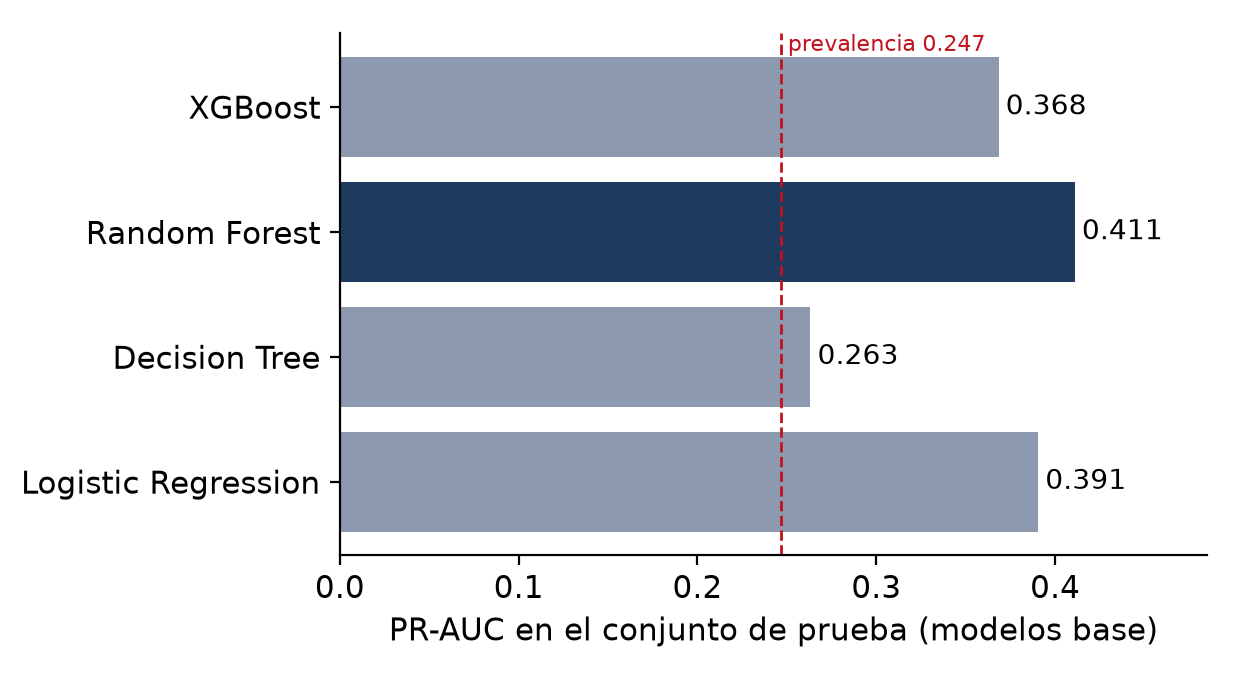
\includegraphics[width=0.7\textwidth]{figuras/comparacion-modelos.png}
  \caption{Comparación de los cuatro modelos base por PR-AUC en el conjunto de prueba. Elaboración propia.}
  \label{fig:comparacion}
\end{figure}

\subsection{API y tablero}
La API carga el \textit{Pipeline} serializado, valida que la solicitud contenga exactamente las 114 variables y devuelve la clase, la probabilidad y un nivel de riesgo. La clase se asigna con el umbral de 0.42. El tablero en React consume la API para mostrar indicadores, métricas y los módulos de clasificación individual y por archivo (Anexo~B). Su interfaz se revisó y corrigió durante la elaboración de este documento (cambios publicados en el repositorio, Anexo~E).

\section{Pruebas y Validación}
Se realizaron dos tipos de pruebas, que evalúan aspectos distintos y no deben confundirse:
\begin{itemize}
  \item \textbf{Evaluación del modelo:} desempeño predictivo sobre la partición de prueba (interna) y sobre su subconjunto de Tungurahua. No es una validación externa, porque la partición proviene de la misma encuesta y el mismo protocolo.
  \item \textbf{Pruebas funcionales de la API:} verifican que el servicio responda según su contrato. Un resultado favorable indica que el software funciona, no que la predicción sea válida clínicamente.
\end{itemize}

Las pruebas funcionales incluyeron 17 casos (Anexo~C) y las 21 pruebas automáticas del repositorio. Las 21 pruebas y 16 de los 17 casos se cumplieron; falló CP15 (la puntuación del formulario individual casi no varía con los datos). CP14 (archivo Excel enviado directamente a la API) falló en la versión evaluada inicialmente y se volvió a ejecutar con el servicio corregido (Anexo~C). La latencia de \texttt{POST /predict}, medida en 100 solicitudes en ejecución local (sin red), tuvo mediana de 29 ms, percentil 95 de 33 ms y máximo de 38 ms. Como comprobación de consistencia, la probabilidad devuelta por la API para un registro coincidió con la calculada directamente sobre el modelo (0.437).

\section{Resultados}
\subsection{Desempeño en el conjunto de prueba nacional}
La Tabla~\ref{tab:metricas} presenta las métricas con el umbral de 0.42, con intervalos de confianza del \SI{95}{\percent} obtenidos por \textit{bootstrap} (1000 remuestreos). La Figura~\ref{fig:matriz} muestra la matriz de confusión y la Figura~\ref{fig:curvas} las curvas ROC y de precisión--sensibilidad.

De los 912 niños con desnutrición crónica del conjunto de prueba, el modelo identificó 632 (sensibilidad de 0.693). A cambio, clasificó como positivos a \num{1255} de los \num{2787} niños sin desnutrición (especificidad de 0.550), por lo que solo una de cada tres alertas es un caso real (precisión de 0.335, frente a una prevalencia de 0.247). El ROC-AUC de 0.677 indica una capacidad de discriminación moderada.

\begin{table}[H]
  \caption{Métricas del modelo en el conjunto de prueba nacional ($n$~=~\num{3699}, umbral 0.42).}
  \label{tab:metricas}
  \tablabase\small
  \begin{tabular}{|p{5.6cm}|c|c|}
    \hline
    \enc{Métrica} & \enc{Valor} & \enc{IC 95\,\%}\\ \hline
    Sensibilidad (clase 1) & 0.693 & 0.664--0.723\\ \hline
    Especificidad (clase 0) & 0.550 & ---\\ \hline
    Precisión (clase 1) & 0.335 & ---\\ \hline
    F1 (clase 1) & 0.452 & 0.429--0.473\\ \hline
    Exactitud balanceada & 0.621 & ---\\ \hline
    ROC-AUC & 0.677 & 0.657--0.696\\ \hline
    PR-AUC (referencia: 0.247) & 0.409 & 0.377--0.442\\ \hline
  \end{tabular}
\end{table}

\begin{figure}[H]
  \centering
  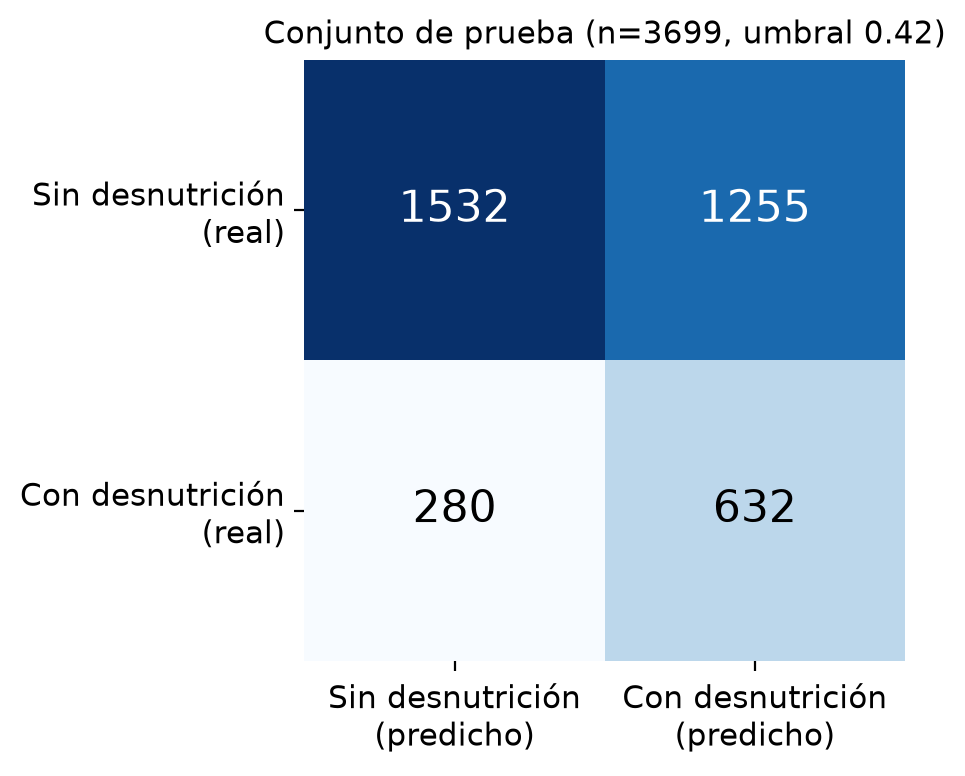
\includegraphics[width=0.55\textwidth]{figuras/matriz-confusion-global.png}
  \caption{Matriz de confusión en el conjunto de prueba nacional (umbral 0.42). Elaboración propia.}
  \label{fig:matriz}
\end{figure}

\begin{figure}[H]
  \centering
  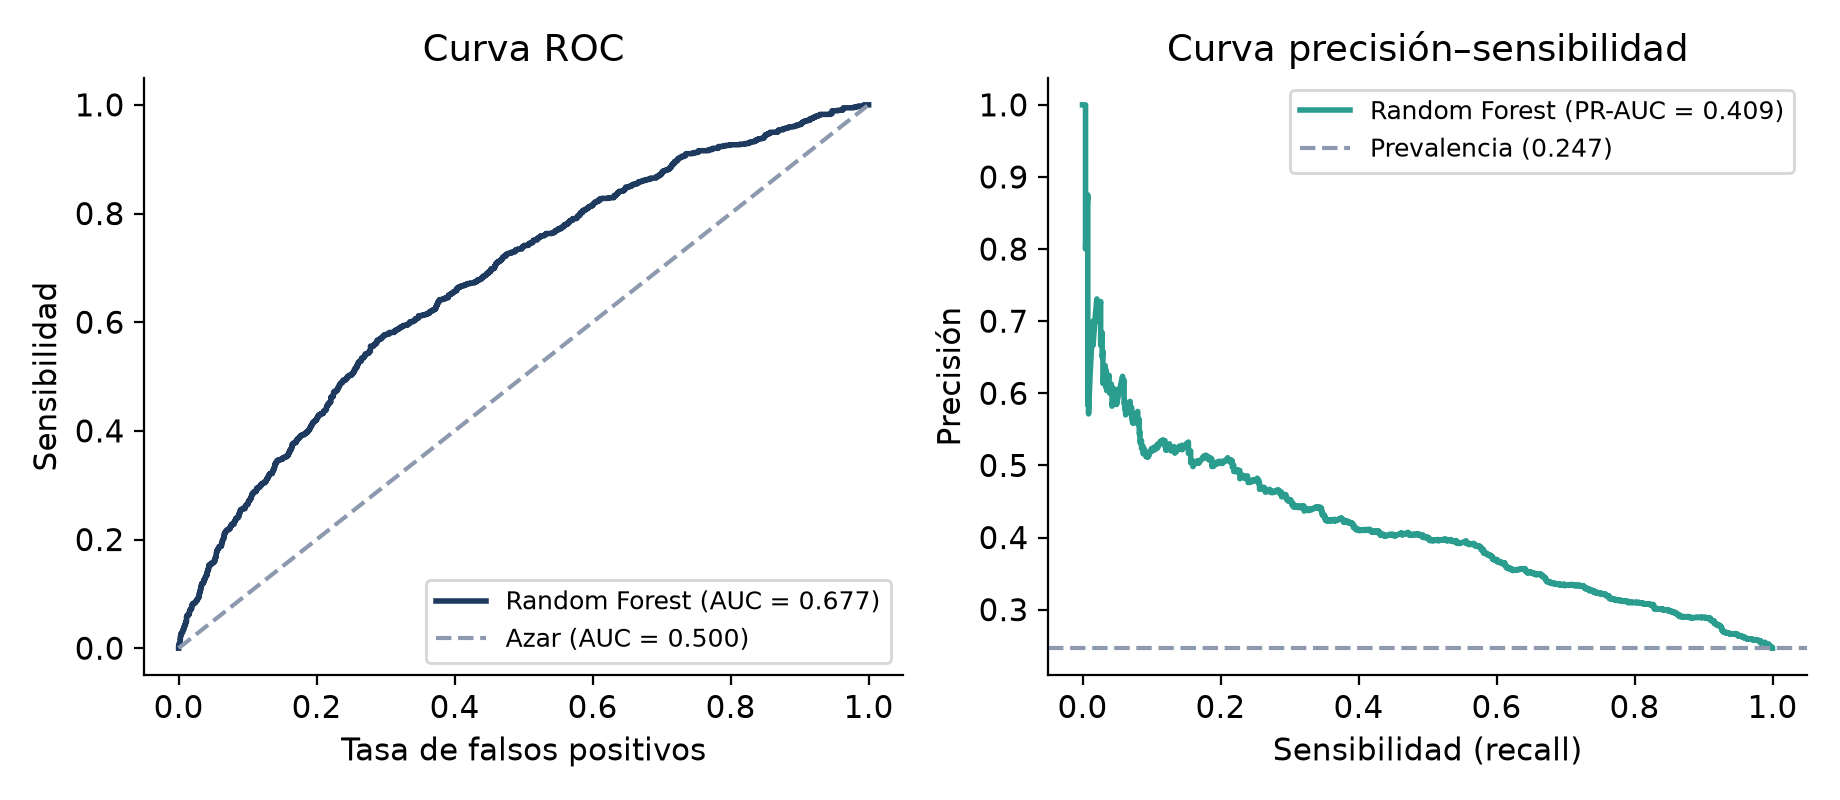
\includegraphics[width=0.95\textwidth]{figuras/curvas-roc-pr.png}
  \caption{Curvas ROC y de precisión--sensibilidad del modelo final en el conjunto de prueba. Elaboración propia.}
  \label{fig:curvas}
\end{figure}

\subsection{Desempeño en Tungurahua}
El conjunto de prueba contiene 112 registros de Tungurahua (35 con desnutrición crónica). La Tabla~\ref{tab:tung} los compara con el resto del país. Los valores puntuales son similares, pero el intervalo de Tungurahua es amplio (por ejemplo, la sensibilidad va de 0.533 a 0.833) debido al tamaño de la muestra. Por ello los resultados de Tungurahua son indicativos y no permiten afirmar que el modelo funcione mejor o peor allí que en el resto del país.

\begin{table}[H]
  \caption{Métricas del modelo en Tungurahua y en el resto del país (conjunto de prueba, umbral 0.42).}
  \label{tab:tung}
  \tablabase\small
  \begin{tabular}{|p{4.4cm}|c|c|c|}
    \hline
    \enc{Métrica} & \enc{Tungurahua} & \enc{IC 95\,\% (Tung.)} & \enc{Resto del país}\\ \hline
    Registros (casos) & 112 (35) & --- & \num{3587} (877)\\ \hline
    Sensibilidad & 0.686 & 0.533--0.833 & 0.693\\ \hline
    Especificidad & 0.571 & --- & 0.549\\ \hline
    Precisión & 0.421 & --- & 0.332\\ \hline
    F1 (clase 1) & 0.522 & 0.385--0.641 & 0.449\\ \hline
    Exactitud balanceada & 0.629 & --- & 0.621\\ \hline
    ROC-AUC & 0.667 & 0.559--0.766 & 0.678\\ \hline
    PR-AUC & 0.485 & 0.336--0.635 & 0.408\\ \hline
  \end{tabular}
\end{table}

\begin{figure}[H]
  \centering
  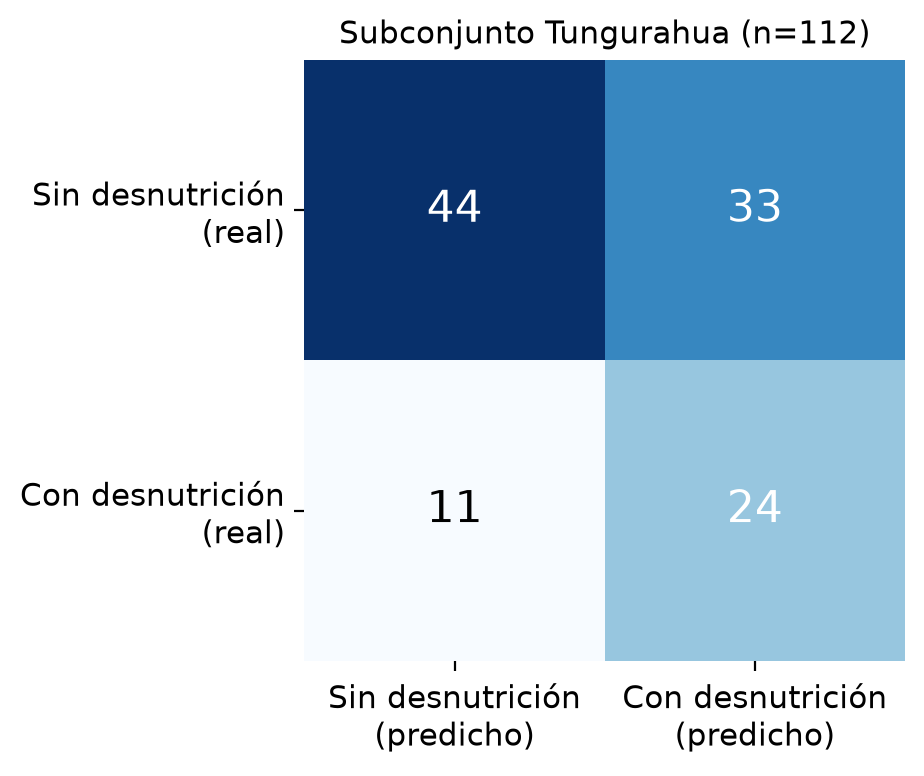
\includegraphics[width=0.5\textwidth]{figuras/matriz-confusion-tungurahua.png}
  \caption{Matriz de confusión en el subconjunto de Tungurahua del conjunto de prueba. Elaboración propia.}
  \label{fig:matriz-tung}
\end{figure}

\subsection{Sobreajuste}
El modelo se ajusta mucho mejor al entrenamiento que a la prueba (Tabla~\ref{tab:sobreajuste}): la exactitud balanceada baja de 0.819 a 0.621 y el PR-AUC de 0.815 a 0.409. Se limitó la profundidad de los árboles (20) y el tamaño de las hojas (10), pero la brecha persiste y debe considerarse al interpretar cualquier resultado.

\begin{table}[H]
  \caption{Comparación entre entrenamiento y prueba (umbral 0.42).}
  \label{tab:sobreajuste}
  \tablabase\small
  \begin{tabular}{|p{5.2cm}|c|c|}
    \hline
    \enc{Métrica} & \enc{Entrenamiento} & \enc{Prueba}\\ \hline
    Sensibilidad (clase 1) & 0.970 & 0.693\\ \hline
    Precisión (clase 1) & 0.489 & 0.335\\ \hline
    Exactitud balanceada & 0.819 & 0.621\\ \hline
    ROC-AUC & 0.932 & 0.677\\ \hline
    PR-AUC & 0.815 & 0.409\\ \hline
  \end{tabular}
\end{table}

\subsection{Comparación de los cuatro modelos por clase}

La Tabla~\ref{tab:modelos4} reporta las métricas de los cuatro modelos base en el conjunto de prueba, cada uno con su propio umbral (el que maximiza el F1 de la clase 1 por validación cruzada en el entrenamiento). Los conteos de las matrices de confusión y las curvas ROC y de precisión--sensibilidad están en el Anexo~H. El mayor PR-AUC correspondió a Random Forest (0.411), el mayor ROC-AUC a Random Forest (0.680), la mayor sensibilidad a XGBoost (0.819) y el mayor F1 a Random Forest (0.459).

La diferencia de PR-AUC entre Random Forest y Regresión logística es de 0.020; es pequeña, por lo que la elección de Random Forest debe leerse como una preferencia débil y no como una superioridad clara.

\begin{table}[H]
  \caption{Métricas de los cuatro modelos base en el conjunto de prueba, con el umbral de cada modelo (F1 máximo por validación cruzada en entrenamiento).}
  \label{tab:modelos4}
  \tablabase\scriptsize
  \begin{tabular}{|l|c|c|c|c|c|c|c|c|}
    \hline
    \enc{Modelo} & \enc{PR-AUC} & \enc{ROC-AUC} & \enc{Umbral} & \enc{Sens.} & \enc{Espec.} & \enc{Prec.} & \enc{F1} & \enc{Ex. bal.} \\ \hline
    Regresión logística & 0.391 & 0.667 & 0.470 & 0.673 & 0.574 & 0.341 & 0.453 & 0.624 \\ \hline
    Árbol de decisión & 0.263 & 0.536 & 0.050 & 0.300 & 0.773 & 0.302 & 0.301 & 0.536 \\ \hline
    Random Forest & 0.411 & 0.680 & 0.230 & 0.735 & 0.521 & 0.334 & 0.459 & 0.628 \\ \hline
    XGBoost & 0.368 & 0.648 & 0.240 & 0.819 & 0.359 & 0.295 & 0.434 & 0.589 \\ \hline
  \end{tabular}
\end{table}




\subsection{Sensibilidad al umbral de decisión}

La Figura~\ref{fig:umbral} muestra cómo cambian las métricas del modelo final al variar el umbral. Con 0.30 la sensibilidad sube a 0.959, pero la precisión baja a 0.261 y el modelo genera 3355 alertas sobre 3699 registros; con 0.42 (umbral adoptado) la sensibilidad es 0.693, la precisión 0.335 y las alertas 1887; con 0.60 la sensibilidad cae a 0.106 y la precisión sube a 0.524. No existe un umbral que alcance a la vez sensibilidad y precisión altas: la elección refleja una decisión sobre qué error se tolera más. Los valores para otros umbrales están en el Anexo~H.

\begin{figure}[H]
  \centering
  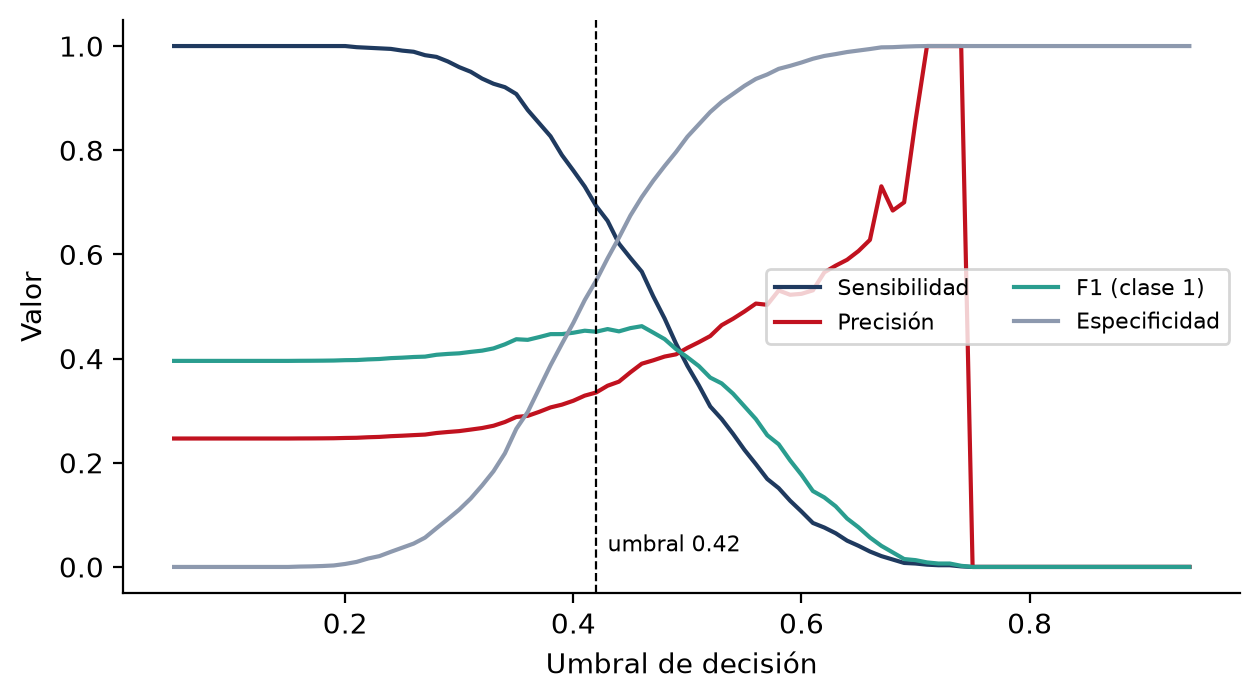
\includegraphics[width=0.75\textwidth]{figuras/anexo-umbral.png}
  \caption{Métricas del modelo final según el umbral de decisión (conjunto de prueba). Elaboración propia.}
  \label{fig:umbral}
\end{figure}



\subsection{Calibración de las probabilidades}

La calibración indica si una probabilidad predicha corresponde a la frecuencia real de casos \cite{steyerberg2019clinical}. El error de Brier del modelo final es 0.205, frente a 0.186 de un predictor que solo usa la prevalencia, es decir, es peor: las probabilidades del modelo no están calibradas. La probabilidad media predicha es 0.427 y la prevalencia observada es 0.247. En el decil más bajo la probabilidad media es 0.264 y la proporción observada 0.105; en el más alto, 0.608 y 0.505.

La probabilidad media supera la prevalencia porque el modelo se entrenó con ponderación de clases; por eso las probabilidades no deben leerse como riesgo absoluto, sino como una puntuación para ordenar casos. Esta es otra razón para no interpretar los niveles de riesgo (BAJO, MEDIO, ALTO) de la API como probabilidades reales. La curva y la distribución de probabilidades están en el Anexo~H (Figura~\ref{fig:calibracion}).



\subsection{Desempeño por subgrupos}

La Figura~\ref{fig:subgrupos} muestra la sensibilidad del modelo final (umbral 0.42) en subgrupos del conjunto de prueba nacional, con intervalos de Wilson. En el conjunto nacional, según el área, la sensibilidad va de 0.525 (Urbano; 480 casos) a 0.880 (Rural; 432 casos); según el sexo, la sensibilidad va de 0.659 (Mujer; 402 casos) a 0.720 (Hombre; 510 casos); según el grupo de edad, la sensibilidad va de 0.505 (36-59; 295 casos) a 0.892 (12-23; 259 casos).

Las diferencias son marcadas: entre Urbano y Rural los intervalos no se traslapan, y la prevalencia muestral es de 21.4\,\% y 29.7\,\% respectivamente; entre 36-59 y 12-23 los intervalos no se traslapan, y la prevalencia muestral es de 19.3\,\% y 34.0\,\% respectivamente. Con un umbral único, el modelo identifica una proporción mayor de los casos donde la prevalencia es mayor y una proporción menor donde es menor. Por eso la sensibilidad global (0.693) oculta diferencias importantes: en los subgrupos con menor prevalencia se omite cerca de la mitad de los casos. Un uso aplicado exigiría revisar el umbral por grupo. En el sexo la diferencia es menor.

El detalle, con especificidad y ROC-AUC, y los subgrupos de Tungurahua (muy pequeños, por lo que solo son indicativos) están en el Anexo~H.

\begin{figure}[H]
  \centering
  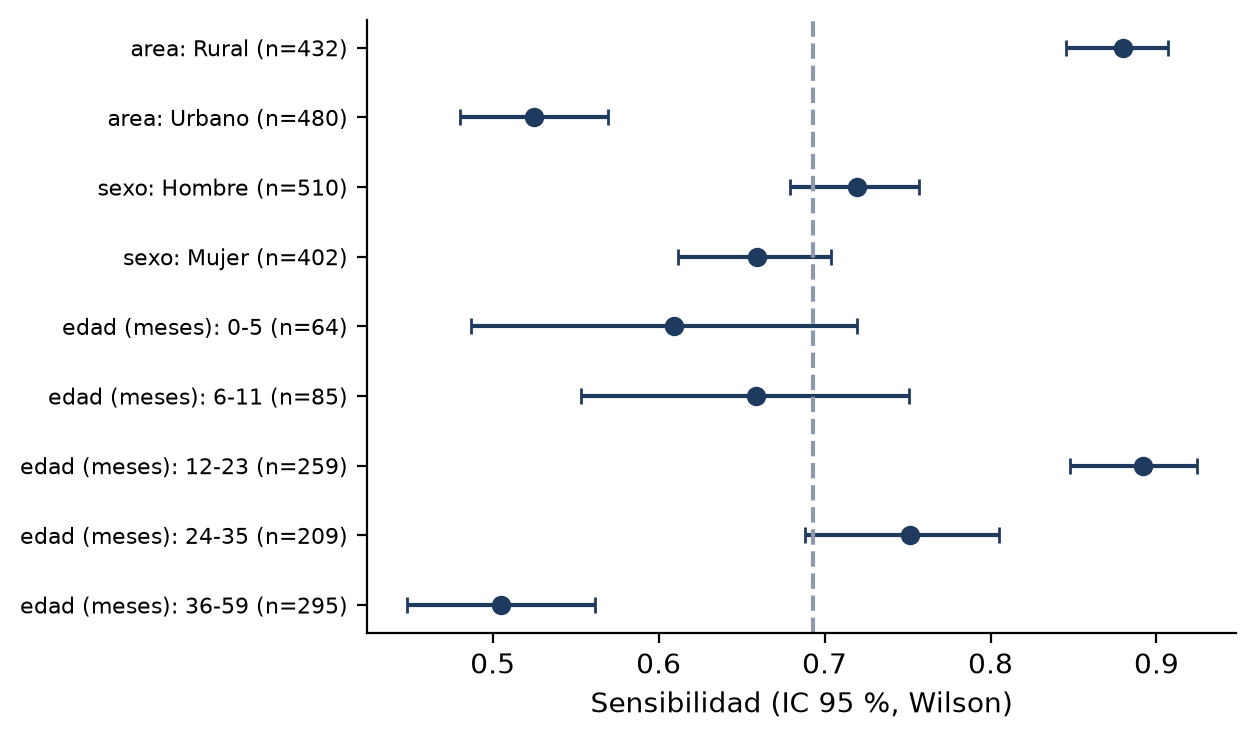
\includegraphics[width=0.8\textwidth]{figuras/anexo-subgrupos.png}
  \caption{Sensibilidad del modelo final por subgrupos en la prueba nacional (línea punteada: sensibilidad global). Elaboración propia.}
  \label{fig:subgrupos}
\end{figure}



\subsection{Análisis de errores}

La Figura~\ref{fig:errores} descompone las clasificaciones por grupo de edad. La proporción de casos omitidos (falsos negativos entre los casos reales) fue mayor en el grupo de 36-59 meses (49.5\,\%) y menor en el de 12-23 meses (10.8\,\%). La proporción de falsas alarmas (falsos positivos entre los no casos) fue mayor en 12-23 meses (75.3\,\%) y menor en 36-59 meses (29.1\,\%). Como la edad es la variable con mayor importancia del modelo, es esperable que los errores dependan de ella; un uso aplicado exigiría revisar el desempeño por edad antes de fijar un umbral único.

\begin{figure}[H]
  \centering
  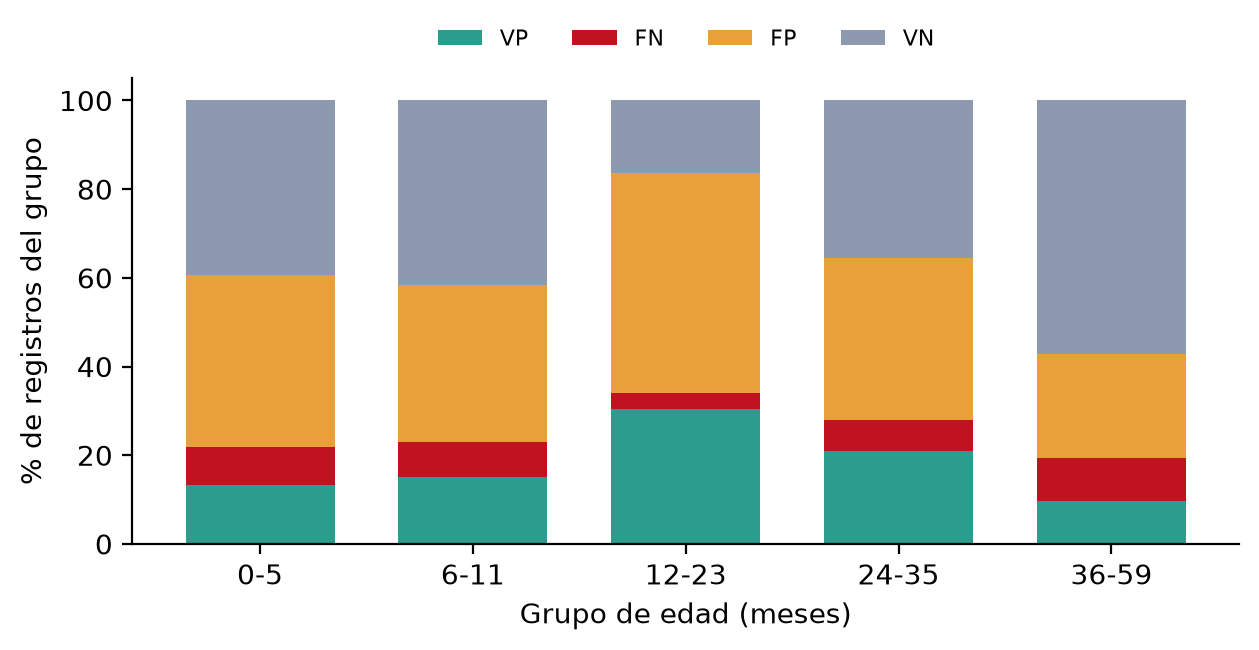
\includegraphics[width=0.75\textwidth]{figuras/anexo-errores-edad.png}
  \caption{Composición de las clasificaciones por grupo de edad (umbral 0.42). VP: verdaderos positivos; FN: falsos negativos; FP: falsos positivos; VN: verdaderos negativos. Elaboración propia.}
  \label{fig:errores}
\end{figure}



\subsection{Prueba sin las variables de diseño muestral}

Como \texttt{factor\_expansion} y \texttt{estrato} no describen al niño, se entrenó un Random Forest con los mismos hiperparámetros y la misma partición, pero sin esas dos variables. La Tabla~\ref{tab:sindiseno} muestra el resultado: el ROC-AUC pasa de 0.677 a 0.679 (diferencia de +0.002) y el PR-AUC de 0.409 a 0.408 (diferencia de -0.001). La diferencia es pequeña, por lo que el desempeño no depende de forma importante de esas dos variables y el modelo sin ellas es una alternativa más limpia. Con el umbral propio de esta versión (0.40, elegido por validación cruzada en el entrenamiento) la sensibilidad es 0.777 y la precisión 0.319. Esta prueba es un análisis de sensibilidad complementario: el modelo evaluado y desplegado sigue siendo el de 114 variables.

\begin{table}[H]
  \caption{Comparación del modelo final con una versión sin las variables de diseño muestral.}
  \label{tab:sindiseno}
  \tablabase\scriptsize
  \begin{tabular}{|p{5.6cm}|c|c|c|c|c|c|}
    \hline
    \enc{Modelo} & \enc{ROC-AUC} & \enc{PR-AUC} & \enc{Sens.} & \enc{Espec.} & \enc{Prec.} & \enc{Ex. bal.} \\ \hline
    Modelo final (con 114 variables), umbral 0.42 & 0.677 & 0.409 & 0.693 & 0.550 & 0.335 & 0.621 \\ \hline
    Sin \texttt{factor\_expansion} ni \texttt{estrato} (112 variables), umbral 0.42 & 0.679 & 0.408 & 0.717 & 0.540 & 0.338 & 0.629 \\ \hline
    Sin variables de diseño, umbral propio 0.40 & 0.679 & 0.408 & 0.777 & 0.456 & 0.319 & 0.617 \\ \hline
  \end{tabular}
\end{table}





\subsection{Importancia de variables}
La Figura~\ref{fig:importancia} muestra las 15 variables con mayor importancia (suma de sus columnas codificadas). La importancia está repartida: ninguna supera \SI{4.5}{\percent}. Encabezan la lista la edad, el nivel de instrucción de la madre y variables del recién nacido (tamaño y peso al nacer), coherentes con los determinantes descritos en la literatura \cite{nu17223608}. Sin embargo, \texttt{factor\_expansion} y \texttt{estrato}, marcadas en rojo, ocupan el segundo y cuarto lugar. Al ser variables de diseño muestral, su peso puede reflejar la estructura de la encuesta y no características del niño. Además, el peso y la talla al nacer tienen más del \SI{55}{\percent} de valores imputados, por lo que su importancia puede reflejar la ausencia del dato. La importancia de un bosque no implica causalidad.

\begin{figure}[H]
  \centering
  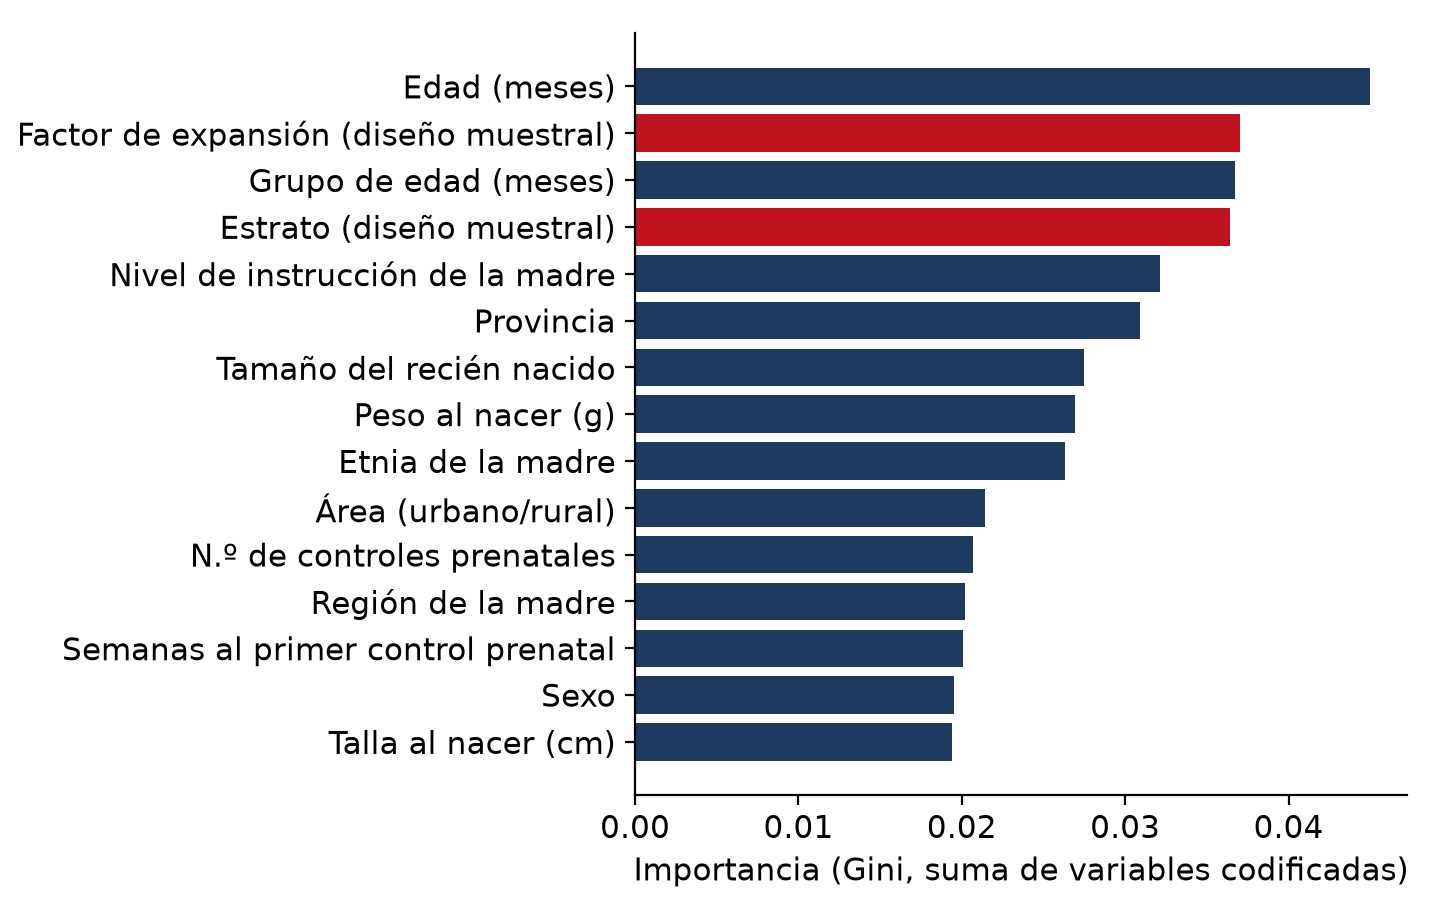
\includegraphics[width=0.85\textwidth]{figuras/importancia-variables.png}
  \caption{Importancia de las 15 variables principales del modelo final. En rojo: variables de diseño muestral. Elaboración propia.}
  \label{fig:importancia}
\end{figure}

\subsection{Comparación con la literatura}
El estudio con datos de la ENDI 2023--2024 reportó AUC de 0.62 a 0.66 para el retraso en talla en niños de 0 a 23 meses \cite{nu18142232}, y el metaanálisis con encuestas DHS, una exactitud agrupada de \SI{68.92}{\percent} \cite{ijerph22030449}. El ROC-AUC de 0.677 obtenido aquí es de magnitud similar al primero. La exactitud global de este modelo con umbral de 0.42 es de 0.585 y no es comparable con la del metaanálisis, porque el umbral se eligió para favorecer la sensibilidad. Los estudios difieren en población, variable objetivo y protocolo, por lo que la comparación es solo referencial.

\subsection{Hallazgos sobre el prototipo}
Las pruebas del sistema revelaron aspectos que deben tenerse en cuenta:
\begin{itemize}
  \item \textbf{Riesgo y clase no coincidían.} En la versión evaluada inicialmente la clase positiva se asignaba con el umbral de 0.42, pero los niveles de riesgo usaban cortes fijos de 0.50 (medio) y 0.80 (alto). En el caso CP4 la API devolvió clase 1 con probabilidad de 0.437 y riesgo BAJO; en la partición de prueba, 1050 de las 1887 clasificaciones positivas (\SI{55.6}{\percent}) figuraban como BAJO y ALTO nunca se alcanzaba (probabilidad máxima de 0.747). Se corrigió: BAJO coincide ahora con la clase 0, MEDIO va de 0.42 a 0.60 y ALTO desde 0.60 (Anexo~A, Tabla~\ref{tab:riesgo}). Los niveles ordenan los casos, pero no son probabilidades calibradas.
  \item \textbf{El resumen del tablero usaba predicciones sobre datos de entrenamiento.} En la versión evaluada inicialmente, \texttt{GET /dashboard} calculaba los ``casos'' como positivos predichos por el modelo sobre el archivo completo (\num{20510} registros, que incluye los usados para entrenar), por lo que no equivalía a la prevalencia observada (\SI{24.7}{\percent}). Se corrigió: el resumen usa el conjunto de prueba (\num{3699} registros que el modelo no vio al entrenar) y muestra juntos los casos observados (912) y los clasificados (\num{1887}), con la sensibilidad y la precisión del ámbito, que reproducen las métricas del modelo (0.693 y 0.335). En Tungurahua (112 registros) hay 35 casos observados y 57 clasificados, con una sensibilidad de 0.686 que es inestable por el tamaño de la muestra.
  \item \textbf{Imputación previa a la partición y muy alta en variables clave.} Los faltantes se imputaron antes de dividir los datos, y variables muy importantes del modelo tienen más de la mitad de sus valores imputados (peso y talla al nacer). Como un valor imputado coincide con la mediana, el modelo puede estar usando el hecho de que el dato faltaba y no el valor real; su importancia debe interpretarse con esa reserva.
  \item \textbf{El formulario de clasificación individual solo es ilustrativo.} La versión inicial del tablero pedía 8 datos y completaba las otras 106 variables con el valor 0 (y las categóricas con códigos numéricos que el modelo no vio en el entrenamiento): en 270 combinaciones la probabilidad varió solo de 0.436 a 0.512 y todas quedaron clasificadas con desnutrición. Se corrigió: el formulario envía las 114 variables (las no informadas como nulas, que el \textit{Pipeline} imputa) con las categorías válidas y la edad agrupada correcta. Aun así, en 512 combinaciones de prueba la probabilidad varió solo de 0.375 a 0.515 y el \SI{85.5}{\percent} quedó clasificado con desnutrición (CP15), porque el resto de las variables se imputa. Por eso la pantalla lo declara de uso ilustrativo y remite a la clasificación por archivo.
  \item \textbf{Carga de archivos Excel.} La pantalla mencionaba archivos \texttt{.xlsx}, pero en la versión evaluada inicialmente el servicio solo leía CSV y un Excel enviado a la API producía una excepción no controlada (CP14). Se corrigió: la API lee \texttt{.xlsx} y devuelve el mismo resultado que con el CSV equivalente, y ante un Excel dañado, un \texttt{.xls}, un archivo vacío o sin registros responde con un mensaje de error en lugar de una excepción. El tablero acepta solo CSV y muestra un mensaje claro con las columnas faltantes (CP16).
  \item \textbf{Página de métricas del tablero.} Leía los nombres de métricas de la versión anterior (\texttt{accuracy}, \texttt{recall}\ldots) y con la API v2 habría mostrado valores no numéricos; se actualizó para mostrar la sensibilidad, la precisión, el F1, la exactitud balanceada, el ROC-AUC y el PR-AUC de \texttt{metricas\_v2.json}.
  \item \textbf{Lenguaje de la interfaz.} La interfaz inicial usaba términos clínicos (``Sistema ML Clínico'', ``Predicción Clínica'', ``alto grado de confianza clínica'') y mencionaba XGBoost, aunque el modelo activo es Random Forest. Se corrigió: todas las pantallas muestran un aviso de herramienta académica exploratoria, se retiró el lenguaje clínico, el nombre del modelo se lee de la API y el resumen de indicadores aclara que las cifras son del conjunto de prueba y no la prevalencia poblacional (Anexo~B).
\end{itemize}

\subsection{Síntesis de resultados}
La Tabla~\ref{tab:cumplimiento} indica el estado de cada requerimiento según la evidencia de este capítulo.

\begin{table}[H]
  \caption{Cumplimiento de los requerimientos.}
  \label{tab:cumplimiento}
  \tablabase\footnotesize
  \begin{tabular}{|c|c|p{9.4cm}|}
    \hline
    \enc{ID} & \enc{Estado} & \enc{Evidencia}\\ \hline
    RF1 & Cumple & Pipeline con preprocesamiento ajustado solo en entrenamiento; semilla 42\\ \hline
    RF2 & Cumple & Tabla~\ref{tab:experimento}, Tabla~\ref{tab:metricas} y Figura~\ref{fig:comparacion}\\ \hline
    RF3 & Cumple & CP4 a CP7 (Anexo~C)\\ \hline
    RF4 & Cumple & CP8: un CSV de 50 registros devuelve 50 filas; CP14: un Excel de 50 registros devuelve 50 filas y los archivos inválidos reciben un mensaje de error\\ \hline
    RF5 & Cumple & CP11: métricas idénticas a \texttt{metricas\_v2.json}\\ \hline
    RF6 & Cumple & CP9, CP10 y CP12: el resumen usa el conjunto de prueba y reproduce las métricas de \texttt{metricas\_v2.json}\\ \hline
    RF7 & Cumple & CP13\\ \hline
    RF8 & Cumple & Prueba de contrato de versión del modelo\\ \hline
    RNF1 & Cumple & CP5, CP6 y CP7: HTTP 400 en los tres casos\\ \hline
    RNF2 & Cumple & Mediana de 29 ms en 100 solicitudes (local)\\ \hline
    RNF3 & Cumple & CP1 (\texttt{GET /health}). No se midió disponibilidad en el tiempo\\ \hline
    RNF4 & No cumple & La API no implementa autenticación; el CORS está abierto\\ \hline
    RNF5 & Cumple & Semilla y versiones fijadas en \texttt{requirements.txt}\\ \hline
    RNF6 & Cumple & Módulos separados y 21 pruebas automáticas aprobadas\\ \hline
    RNF7 & Cumple & Aviso académico visible en todas las pantallas y lenguaje clínico retirado (Anexo~B)\\ \hline
  \end{tabular}
\end{table}

En síntesis, el prototipo cumple 14 de los 15 requerimientos y 1 no se cumple. El modelo tiene un desempeño moderado (ROC-AUC de 0.677), sobreajuste medido y ninguna validación externa; sus productos son una API funcional con datos completos y un tablero de consulta cuyo formulario individual solo es ilustrativo. Quedan pendientes la autenticación y la validación con una fuente independiente.

\section{Cronograma y Presupuesto}
\subsection{Cronograma de Ejecución}
La Tabla~\ref{tab:cronograma} presenta las actividades ejecutadas. \pend{verificar las fechas reales de cada actividad; las anteriores a septiembre provienen de la versión previa del documento}

\begingroup
\footnotesize\setlength{\tabcolsep}{4pt}\arrayrulecolor{black!55}\renewcommand{\arraystretch}{1.1}
\begin{longtable}{|c|p{5.2cm}|c|c|p{2.8cm}|}
  \caption{Cronograma de actividades del proyecto.}
  \label{tab:cronograma}\\ \hline
  \enc{N.º} & \enc{Actividad} & \enc{Inicio} & \enc{Fin} & \enc{Resultado}\\ \hline
  \endfirsthead
  \tablacont{5}\hline
  \enc{N.º} & \enc{Actividad} & \enc{Inicio} & \enc{Fin} & \enc{Resultado}\\ \hline
  \endhead
  \hline\endfoot
  1 & Revisión bibliográfica y definición del problema & 04/05/2026 & 08/05/2026 & Marco conceptual\\ \hline
  2 & Recopilación y revisión de los datos ENSANUT (y exploración de ENDI) & 09/05/2026 & 12/05/2026 & Datos brutos\\ \hline
  3 & Auditoría técnica y análisis exploratorio & 13/05/2026 & 20/05/2026 & Diagnóstico de calidad\\ \hline
  4 & Limpieza y preparación de variables & 21/05/2026 & 29/05/2026 & Dataset preparado\\ \hline
  5 & Entrenamiento inicial de modelos (v1) & 30/05/2026 & 06/06/2026 & Modelos base\\ \hline
  6 & Optimización de hiperparámetros (v1) & 07/06/2026 & 13/06/2026 & Modelo optimizado\\ \hline
  7 & Evaluación y selección del modelo (v1) & 14/06/2026 & 18/06/2026 & Modelo seleccionado\\ \hline
  8 & Serialización del modelo & 19/06/2026 & 21/06/2026 & Archivo \texttt{.joblib}\\ \hline
  9 & Desarrollo de la API REST & 22/06/2026 & 30/06/2026 & Servicios implementados\\ \hline
  10 & Pruebas funcionales de la API & 01/07/2026 & 04/07/2026 & API verificada\\ \hline
  11 & Redacción de la primera versión del documento & 05/07/2026 & 13/07/2026 & Documento inicial\\ \hline
  12 & Revisión del pipeline y reentrenamiento (v2) & 12/09/2026 & 13/09/2026 & Modelo v2 y métricas\\ \hline
  13 & Integración de v2 en la API y pruebas de contrato & 13/09/2026 & 13/09/2026 & API con v2\\ \hline
  14 & Reestructuración del documento según observaciones & 14/09/2026 & 20/09/2026 & Documento corregido\\ \hline
\end{longtable}
\endgroup

\subsection{Presupuesto}
El desarrollo usó software libre y un equipo del investigador. La Tabla~\ref{tab:presupuesto} presenta el presupuesto estimado. \pend{confirmar los montos reales de conectividad, energía, servicios en la nube e impresión}

\begin{table}[H]
  \caption{Presupuesto estimado del proyecto.}
  \label{tab:presupuesto}
  \tablabase\footnotesize
  \begin{tabular}{|p{4.2cm}|c|c|r|}
    \hline
    \enc{Recurso} & \enc{Cantidad} & \enc{Costo unitario (USD)} & \enc{Subtotal (USD)}\\ \hline
    Equipo informático (propio) & 1 & 0.00 & 0.00\\ \hline
    Software libre (Python, FastAPI, scikit-learn, React) & 1 & 0.00 & 0.00\\ \hline
    Conexión a internet & 2 meses & 25.00 & 50.00\\ \hline
    Energía eléctrica & 2 meses & 15.00 & 30.00\\ \hline
    Servicios en la nube (pruebas de despliegue) & 1 & 20.00 & 20.00\\ \hline
    Impresión y encuadernación & 1 & 25.00 & 25.00\\ \hline
    Contingencias & 1 & 25.00 & 25.00\\ \hline
    \textbf{Total estimado} & & & \textbf{150.00}\\ \hline
  \end{tabular}
\end{table}

\chapter{Conclusiones y Recomendaciones}

\section{Conclusiones}
Se desarrolló y evaluó un prototipo académico de clasificación de la desnutrición crónica infantil con microdatos de la ENSANUT 2018. Las conclusiones siguientes corresponden a cada objetivo específico y se sustentan en los resultados del Capítulo~III.

\noindent\hspace*{\parindent}\textbf{Objetivo 1: análisis y preparación de datos.} La base original tenía \num{20510} registros y 350 variables; \num{2017} registros (\SI{9.8}{\percent}) carecían de la variable objetivo y se excluyeron en lugar de imputarse, con lo que se conservaron \num{18493} registros y 114 predictores. Los predictores no incluyen talla ni peso actuales del niño, pero sí dos variables de diseño muestral (\texttt{factor\_expansion} y \texttt{estrato}) que pueden condicionar los resultados. Además, 84 de los 114 predictores tenían valores ausentes (32 con más del \SI{10}{\percent}), que se imputaron antes de la partición.

\noindent\hspace*{\parindent}\textbf{Objetivo 2: diseño de la arquitectura y del protocolo.} La solución se organizó en cuatro componentes (pipeline, artefactos, API y tablero). El protocolo fijó una partición 80/20 estratificada con semilla 42, un preprocesamiento dentro del \textit{Pipeline}, la selección por PR-AUC y un umbral de decisión de 0.42. Se definieron 8 requerimientos funcionales y 7 no funcionales con criterios de aceptación.

\noindent\hspace*{\parindent}\textbf{Objetivo 3: entrenamiento, comparación y evaluación.} Random Forest obtuvo el mayor PR-AUC entre los cuatro modelos (0.411). Con el modelo final, en el conjunto de prueba nacional (n = \num{3699}), la sensibilidad fue de 0.693, la precisión de 0.335, el F1 de 0.452, la exactitud balanceada de 0.621, el ROC-AUC de 0.677 y el PR-AUC de 0.409. En Tungurahua (n = 112) la sensibilidad fue de 0.686 con intervalo de \SI{95}{\percent} de 0.533 a 0.833. El desempeño es moderado y comparable con el reportado con datos de la ENDI (AUC de 0.62 a 0.66), y el modelo presenta sobreajuste (exactitud balanceada de 0.819 en entrenamiento frente a 0.621 en prueba).

\noindent\hspace*{\parindent}\textbf{Objetivo 4: API y tablero.} Se implementó una API REST con nueve servicios, que valida las 114 variables de entrada, y un tablero web que consume la API para consultar indicadores, métricas y predicciones.

\noindent\hspace*{\parindent}\textbf{Objetivo 5: validación funcional y limitaciones.} Las 8 pruebas automáticas y 15 de los 17 casos de prueba se cumplieron (fallaron el envío de un Excel a la API y la variación de la puntuación del formulario individual), y la latencia mediana fue de 29 ms en ejecución local. Estas pruebas verifican el funcionamiento del software y no la validez predictiva ni clínica. Se identificó que el nivel de riesgo contradecía la clase asignada (corregido: BAJO coincide ahora con la clase 0), que el resumen del tablero usa predicciones sobre datos de entrenamiento, que la puntuación del formulario individual casi no varía con los datos porque el resto de las variables se imputa, y que la API no tiene autenticación.

\subsection{Limitaciones}
\begin{itemize}
  \item \textbf{Representatividad territorial:} Tungurahua aporta \num{531} registros (112 en la prueba), por lo que sus estimaciones son imprecisas y no permiten resultados por cantón o parroquia. Las prevalencias reportadas no están ponderadas.
  \item \textbf{Diseño transversal:} el modelo estima la condición observada; no anticipa casos futuros.
  \item \textbf{Desbalance:} la clase de interés es el \SI{24.7}{\percent}; la precisión es baja (una de cada tres alertas es un caso real).
  \item \textbf{Posible fuga o sesgo por variables de diseño:} \texttt{factor\_expansion} y \texttt{estrato} figuran entre las variables más importantes.
  \item \textbf{Imputación previa a la partición:} los faltantes se imputaron con mediana o moda sobre todos los registros antes de dividir los datos, y el peso y la talla al nacer tienen más de la mitad de sus valores imputados. El efecto sobre las métricas no se cuantificó.
  \item \textbf{Selección del modelo:} la comparación de los cuatro modelos base se hizo sobre la partición de prueba, por lo que el PR-AUC de prueba puede ser levemente optimista.
  \item \textbf{Validación externa:} no existe. La ENDI se exploró pero no se usó para validar.
  \item \textbf{Seguridad y reproducibilidad:} la API no autentica usuarios y el CORS está abierto. Los resultados dependen de las versiones de librerías indicadas.
  \item \textbf{Alcance clínico:} el prototipo es una herramienta académica de apoyo analítico; no es un sistema de diagnóstico ni una solución validada para decisiones médicas.
  \item \textbf{Calibración y subgrupos:} las probabilidades no están calibradas y la sensibilidad varía según el área y la edad (Capítulo~III), por lo que un umbral único no es adecuado para un uso aplicado.
\end{itemize}

\subsection{Aportes del trabajo}
\begin{itemize}
  \item \textbf{Procedimiento documentado y corregido:} se detectó y corrigió una fuga en la versión inicial (\num{2017} etiquetas imputadas) y se dejó el procedimiento reproducible, con semilla fija y código disponible (Anexo~I).
  \item \textbf{Evaluación transparente:} se reportaron métricas por clase, intervalos de confianza, sobreajuste, calibración y desempeño por subgrupos, en lugar de una exactitud global.
  \item \textbf{Evaluación para Tungurahua:} se cuantificó el desempeño en la provincia con sus límites de representatividad.
  \item \textbf{Prototipo con pruebas:} se entregó una API con validación de entradas, casos de prueba y una lista explícita de defectos encontrados.
\end{itemize}

\subsection{Lectura conjunta de los análisis complementarios}
Los análisis adicionales del Capítulo~III matizan el desempeño global. Primero, las probabilidades del modelo no están calibradas (error de Brier de 0.205 frente a 0.186 de la prevalencia), por lo que sirven para ordenar casos y no como riesgo absoluto. Segundo, con un umbral único la sensibilidad cambia mucho según el subgrupo: 0.880 en el área rural frente a 0.525 en la urbana, y 0.892 entre los 12 y 23 meses frente a 0.505 entre los 36 y 59 meses. Tercero, excluir las variables de diseño muestral no modifica el ROC-AUC (0.679 frente a 0.677), de modo que el desempeño no depende de ellas. Cuarto, la elección de Random Forest sobre la regresión logística es una preferencia débil: el ROC-AUC de la regresión logística (0.667) y su PR-AUC (0.391) son cercanos a los del bosque (0.680 y 0.411).



\section{Recomendaciones y Trabajos Futuros}
\subsection{Recomendaciones inmediatas}
\begin{itemize}
  \item \textbf{Corregir el resumen del tablero:} calcular los indicadores con los datos observados o con el conjunto de prueba, no con predicciones sobre datos de entrenamiento.
  \item \textbf{Corregir la lectura de archivos en la API:} aceptar Excel o rechazarlo con un error controlado.
  \item \textbf{Decidir el futuro del formulario individual:} mantenerlo solo como ilustración o reemplazarlo por una carga de un registro completo.
  \item \textbf{Proteger la API:} agregar autenticación y restringir el origen de las solicitudes antes de cualquier despliegue abierto.
\end{itemize}

\subsection{Trabajos futuros}
\begin{itemize}
  \item Rehacer la imputación dentro del \textit{Pipeline} a partir de la base original, para cuantificar su efecto, y evaluar con ponderación muestral.
  \item Validar con una fuente independiente, como la ENDI, con una variable objetivo comparable.
  \item Calibrar las probabilidades y analizar la interpretabilidad con métodos como SHAP.
  \item Contrastar el desempeño con profesionales de salud antes de cualquier uso aplicado.
\end{itemize}


%% --- Referencias (IEEE) y glosario ------------------------------------------------
\imprimirreferencias{referencias}
\capitulosinnumero{Glosario}

\section*{Siglas y Acrónimos}
\begin{glosario}
  \termino{API}{Interfaz de Programación de Aplicaciones (\textit{Application Programming Interface}).}
  \termino{AS-IS / TO-BE}{Proceso actual y proceso propuesto.}
  \termino{AUC}{Área bajo la curva (\textit{Area Under the Curve}).}
  \termino{CORS}{Intercambio de recursos entre orígenes (\textit{Cross-Origin Resource Sharing}).}
  \termino{DHS}{Encuestas Demográficas y de Salud (\textit{Demographic and Health Surveys}).}
  \termino{ENDI}{Encuesta Nacional sobre Desnutrición Infantil.}
  \termino{ENSANUT}{Encuesta Nacional de Salud y Nutrición.}
  \termino{FN, FP, VN, VP}{Falsos negativos, falsos positivos, verdaderos negativos y verdaderos positivos.}
  \termino{HTTP}{Protocolo de transferencia de hipertexto (\textit{HyperText Transfer Protocol}).}
  \termino{IC}{Intervalo de confianza.}
  \termino{INEC}{Instituto Nacional de Estadística y Censos.}
  \termino{JSON}{Notación de objetos de JavaScript (\textit{JavaScript Object Notation}).}
  \termino{ML}{Aprendizaje automático (\textit{Machine Learning}).}
  \termino{ODS}{Objetivos de Desarrollo Sostenible.}
  \termino{OMS}{Organización Mundial de la Salud.}
  \termino{OSEMN}{\textit{Obtain, Scrub, Explore, Model, iNterpret}.}
  \termino{PR-AUC}{Área bajo la curva de precisión--sensibilidad (\textit{average precision}).}
  \termino{REST}{Transferencia de Estado Representacional (\textit{Representational State Transfer}).}
  \termino{ROC}{Característica operativa del receptor (\textit{Receiver Operating Characteristic}).}
  \termino{SHAP}{Explicaciones aditivas de Shapley (\textit{SHapley Additive exPlanations}).}
\end{glosario}

\section*{Glosario de Términos}
\begin{glosario}
  \termino{Bootstrap}{Técnica que remuestrea con reemplazo los datos de prueba para estimar la variabilidad de una métrica y su intervalo de confianza.}
  \termino{Brier (error de)}{Promedio del cuadrado de la diferencia entre la probabilidad predicha y el resultado observado; mide la calibración y la precisión de las probabilidades.}
  \termino{Calibración}{Grado en que las probabilidades predichas coinciden con las frecuencias observadas.}
  \termino{Clasificación}{Tarea de asignar cada registro a una categoría; aquí, con o sin desnutrición crónica.}
  \termino{Desnutrición crónica}{Retraso del crecimiento en talla para la edad, asociado a deficiencias nutricionales prolongadas.}
  \termino{Desbalance de clases}{Situación en que una categoría tiene muchos menos registros que otra.}
  \termino{Diseño transversal}{Estudio en el que cada unidad se mide una sola vez, por lo que no permite anticipar eventos futuros.}
  \termino{Especificidad}{Proporción de casos negativos que el modelo identifica correctamente.}
  \termino{Estrato}{Variable de diseño muestral que agrupa unidades de la encuesta; no describe al niño.}
  \termino{Exactitud balanceada}{Promedio de la sensibilidad y la especificidad.}
  \termino{Factor de expansión}{Peso que indica a cuántas unidades de la población representa un registro de la encuesta.}
  \termino{Fuga de información}{Uso, durante el entrenamiento, de datos que revelan la variable objetivo o la partición de prueba.}
  \termino{One-hot}{Codificación de una variable categórica en columnas binarias, una por categoría.}
  \termino{Pipeline}{Secuencia de pasos de preprocesamiento y modelado que se ajusta como una sola unidad.}
  \termino{Precisión}{Proporción de positivos predichos que son casos reales.}
  \termino{Prevalencia}{Proporción de casos en una población o muestra en un momento dado.}
  \termino{Random Forest}{Modelo que promedia muchos árboles de decisión entrenados con muestras aleatorias.}
  \termino{Sensibilidad}{Proporción de casos positivos que el modelo identifica correctamente.}
  \termino{Sobreajuste}{Situación en que un modelo se ajusta al entrenamiento mucho mejor que a datos nuevos.}
  \termino{Tamizaje}{Aplicación de una prueba a una población para detectar posibles casos.}
  \termino{Umbral de decisión}{Probabilidad a partir de la cual el modelo asigna la clase positiva.}
  \termino{Validación cruzada}{Procedimiento que divide el entrenamiento en particiones para ajustar y evaluar sin usar la prueba.}
  \termino{Validación externa}{Evaluación con datos de otra fuente, población o periodo distintos de los usados para entrenar.}
\end{glosario}


%% --- Anexos -------------------------------------------------------------------------
%% ============================================================================
%%  Anexos A–I. Cada uno abre con su página divisoria (macro \anexo).
%%  No se incluyen cartas, actas ni instrumentos de campo: no existe entidad
%%  receptora ni se aplicaron entrevistas o encuestas (ver Capítulo II).
%% ============================================================================

%% ----------------------------------------------------------------- ANEXO A
\anexo{A}{Documentación Técnica del Sistema}

\section*{A.1 Estructura del repositorio}
\begin{table}[H]
  \caption{Módulos principales del backend (\texttt{API\_DESNUTRICION/backend}).}
  \label{tab:modulos}
  \tablabase\footnotesize
  \begin{tabular}{|p{4.0cm}|p{9.4cm}|}
    \hline
    \enc{Archivo} & \enc{Función}\\ \hline
    \texttt{app/main.py} & Definición de rutas de la API y validación de solicitudes\\ \hline
    \texttt{app/predictor.py} & Carga del \textit{Pipeline}, validación de variables y predicción\\ \hline
    \texttt{app/predict\_file.py} & Procesamiento de archivos para predicción masiva\\ \hline
    \texttt{app/dashboard.py} & Resumen de indicadores por provincia\\ \hline
    \texttt{app/analytics.py} & Métricas del modelo e importancia de variables\\ \hline
    \texttt{app/schemas.py} & Esquema de respuesta de \texttt{/predict}\\ \hline
    \texttt{app/config.py} & Rutas, versión del modelo y umbral de decisión\\ \hline
    \texttt{app/utils.py} & Validación de variables y catálogo de provincias\\ \hline
    \texttt{models/} & \texttt{modelo\_v2.joblib}, \texttt{modelo\_final\_api.joblib} (v1) y \texttt{metricas\_v2.json}\\ \hline
    \texttt{data/} & Conjunto de prueba (\texttt{test\_v2.csv}) que usa el resumen del tablero y otros datos del proyecto\\ \hline
    \texttt{tests/} & Pruebas de contrato de la API, de las métricas, del nivel de riesgo, del resumen del tablero y de la lectura de archivos\\ \hline
  \end{tabular}
\end{table}

\begin{table}[H]
  \caption{Módulos principales del tablero (\texttt{API\_DESNUTRICION/frontend/src}).}
  \label{tab:modulos-front}
  \tablabase\footnotesize
  \begin{tabular}{|p{4.8cm}|p{8.6cm}|}
    \hline
    \enc{Archivo} & \enc{Función}\\ \hline
    \texttt{pages/Home.tsx} & Pantalla de inicio\\ \hline
    \texttt{pages/Dashboard.tsx} & Indicadores por provincia\\ \hline
    \texttt{pages/PredictionForm.tsx} & Formulario de predicción individual\\ \hline
    \texttt{pages/BatchPrediction.tsx} & Carga de archivo para predicción masiva\\ \hline
    \texttt{pages/Metrics.tsx} & Métricas del modelo e importancia de variables\\ \hline
    \texttt{services/api.ts} & Funciones que llaman a la API con \textit{axios}\\ \hline
    \texttt{components/} & Barra lateral, contenedores y ayudas emergentes\\ \hline
  \end{tabular}
\end{table}

\section*{A.2 Configuración}
La variable de entorno \texttt{MODEL\_VERSION} selecciona el modelo activo: \texttt{v2} (por defecto) o \texttt{v1}. El umbral de decisión de la versión v2 se lee de \texttt{metricas\_v2.json} (0.42); la versión v1 usa 0.5. El servicio se inicia en Render con \texttt{uvicorn app.main:app --host 0.0.0.0 --port 10000}, y el tablero usa la variable \texttt{VITE\_API\_URL} para ubicar la API cuando se despliega en Vercel.

\begin{table}[H]
  \caption{Dependencias del backend (\texttt{requirements.txt}).}
  \label{tab:deps}
  \tablabase\small
  \begin{tabular}{|p{4.0cm}|p{3.0cm}|p{5.6cm}|}
    \hline
    \enc{Paquete} & \enc{Versión} & \enc{Uso}\\ \hline
    fastapi & 0.116.1 & Servicio REST y documentación OpenAPI\\ \hline
    uvicorn & 0.35.0 & Servidor ASGI\\ \hline
    pandas / numpy & $\geq$ 2.2.3 / $\geq$ 2.1.0 & Manejo de datos\\ \hline
    scikit-learn & 1.6.1 & \textit{Pipeline} y modelos\\ \hline
    xgboost & 2.1.4 & Modelo v1 y candidato\\ \hline
    joblib & 1.5.1 & Carga del modelo serializado\\ \hline
    openpyxl & 3.1.5 & Escritura de resultados \texttt{.xlsx}\\ \hline
    python-multipart & 0.0.20 & Recepción de archivos\\ \hline
    jinja2 & 3.1.6 & Plantilla de la ruta raíz\\ \hline
  \end{tabular}
\end{table}

\section*{A.3 Formato de entrada de \texttt{/predict}}
La solicitud debe contener exactamente las 114 variables del modelo (\texttt{GET /features} las lista y \texttt{GET /example} devuelve una plantilla vacía). Las variables categóricas se envían como texto con las mismas categorías del entrenamiento y las numéricas como números. Los valores no informados pueden enviarse como \texttt{null}; el \textit{Pipeline} los imputa con la mediana o la moda del entrenamiento.

\begin{lstlisting}[frame=single,basicstyle=\ttfamily\footnotesize]
POST /predict   (cuerpo JSON con las 114 variables)
{ "area": "Urbano", "provincia": 18, "sexo": "Mujer",
  "edad_meses": 14, "peso_nacer_gramos": 3100, ... }

Respuesta HTTP 200:
{ "prediccion": 1,
  "descripcion": "Con desnutricion cronica",
  "probabilidad": 0.437,
  "riesgo": "MEDIO" }

Respuesta HTTP 400 (variables que no coinciden):
{ "detail": { "mensaje": "Las variables enviadas no
  coinciden con el modelo", "detalle": { ... } } }
\end{lstlisting}

\section*{A.4 Niveles de clase y de riesgo}
La clase se asigna con el umbral de 0.42 (probabilidad $\geq$ 0.42: clase 1). El nivel de riesgo se deriva del mismo umbral: BAJO si la probabilidad es menor que 0.42 (clase 0), MEDIO si está entre 0.42 y 0.60 y ALTO si es $\geq$ 0.60. Por tanto, ningún caso con clase 1 figura con riesgo BAJO. El corte de ALTO equivale aproximadamente al percentil 95 de las probabilidades del conjunto de prueba.

La versión evaluada inicialmente usaba cortes fijos de 0.50 y 0.80, independientes del umbral: en el conjunto de prueba, 1050 de las 1887 clasificaciones positivas (\SI{55.6}{\percent}) figuraban con riesgo BAJO, y ALTO nunca se alcanzaba (la probabilidad máxima fue 0.747). Se corrigió en el commit \texttt{7b37205} de \texttt{pipeline-v2-fixes} y en el \texttt{588d8fe} de \texttt{main} (Anexo~E). La Tabla~\ref{tab:riesgo} muestra la distribución resultante.

\begin{table}[H]
  \caption{Nivel de riesgo en el conjunto de prueba nacional (n = \num{3699}).}
  \label{tab:riesgo}
  \tablabase\small
  \begin{tabular}{|c|c|c|c|c|}
    \hline
    \enc{Nivel} & \enc{Probabilidad} & \enc{Clase} & \enc{Registros} & \enc{Prevalencia observada}\\ \hline
    BAJO & $<$ 0.42 & 0 & \num{1812} & 0.155\\ \hline
    MEDIO & 0.42 a $<$ 0.60 & 1 & \num{1702} & 0.314\\ \hline
    ALTO & $\geq$ 0.60 & 1 & \num{185} & 0.524\\ \hline
  \end{tabular}
\end{table}

Los niveles ordenan los casos, pero las probabilidades no están calibradas (Capítulo~III); no deben leerse como riesgo absoluto.

\section*{A.5 Ejecución local}
\begin{enumerate}
  \item Backend: crear un entorno virtual, ejecutar \texttt{pip install -r requirements.txt} y luego \texttt{python -m uvicorn app.main:app --reload} (puerto 8000; documentación en \texttt{/docs}).
  \item Frontend: en \texttt{frontend}, ejecutar \texttt{npm install} y \texttt{npm run dev} (puerto 5173).
\end{enumerate}

%% ----------------------------------------------------------------- ANEXO B
\anexo{B}{Manual de Usuario}

\section*{B.1 Aviso de uso}
\noindent\textbf{Herramienta académica exploratoria.} Las salidas del sistema son estimaciones estadísticas obtenidas con un modelo de Machine Learning entrenado con datos de la ENSANUT 2018. No constituyen un diagnóstico clínico, no sustituyen la evaluación de un profesional de salud y no deben usarse para decidir sobre un niño concreto. Este aviso aparece en la parte superior de todas las pantallas.

\section*{B.2 Requisitos de acceso}
El tablero se usa desde un navegador web actual. En ejecución local se abre en \texttt{http://localhost:5173} con la API activa en \texttt{http://localhost:8000}. \pend{indicar las direcciones públicas de la API (Render) y del tablero (Vercel) cuando se publiquen}

\section*{B.3 Navegación}
La barra lateral da acceso a los cinco módulos de la Tabla~\ref{tab:modulos-usuario}. En su parte inferior indica el modelo activo, que se consulta a la API en tiempo real.

\begin{table}[H]
  \caption{Módulos del tablero y su finalidad.}
  \label{tab:modulos-usuario}
  \tablabase\small
  \begin{tabular}{|p{3.6cm}|p{5.8cm}|p{3.6cm}|}
    \hline
    \enc{Módulo} & \enc{Finalidad} & \enc{Servicio de la API}\\ \hline
    Inicio & Presentación y alcance & \texttt{GET /info}\\ \hline
    Clasificación individual & Ilustración con 10 datos & \texttt{POST /predict}\\ \hline
    Clasificación por archivo & Clasificar un CSV de casos & \texttt{POST /predict-file}\\ \hline
    Indicadores & Clasificaciones por provincia & \texttt{GET /dashboard}\\ \hline
    Métricas del modelo & Desempeño e importancia & \texttt{GET /dashboard/}\allowbreak\texttt{metricas}\\ \hline
  \end{tabular}
\end{table}

\section*{B.4 Inicio}
Presenta el alcance del sistema (niños de 0 a 59 meses, ENSANUT 2018, evaluación separada para Tungurahua) y sus límites (Figura~\ref{fig:ui-inicio}).

\begin{figure}[H]
  \centering
  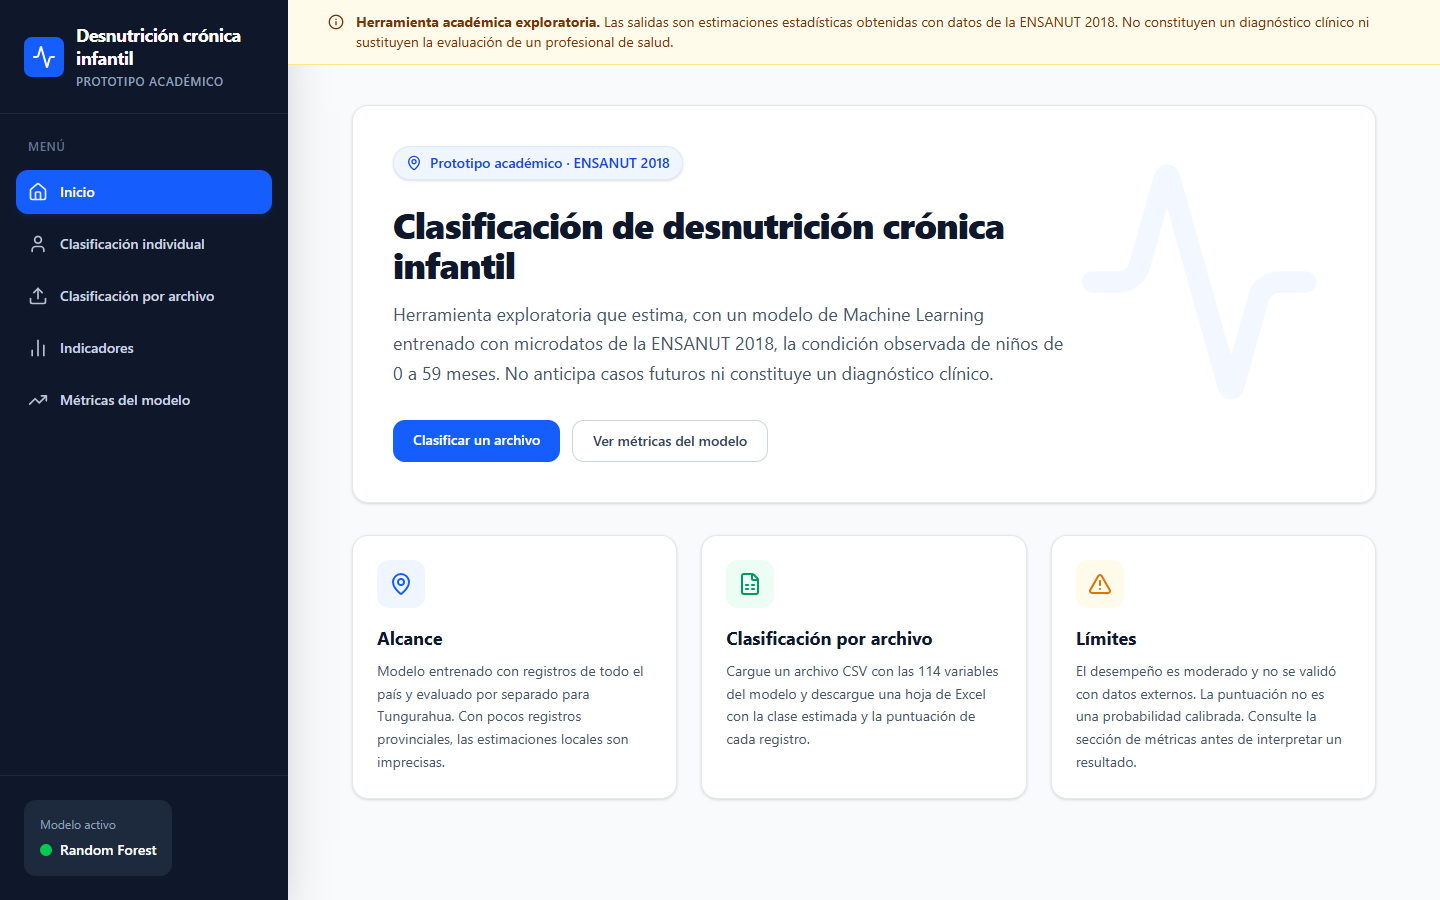
\includegraphics[width=0.85\textwidth]{figuras/ui-inicio.png}
  \caption{Pantalla de inicio del tablero.}
  \label{fig:ui-inicio}
\end{figure}

\section*{B.5 Indicadores}
Muestra, para todo el país o para la provincia elegida en el selector \textit{Ámbito}, los registros de prueba, los casos observados de desnutrición crónica, los que clasifica el modelo y la sensibilidad y la precisión en ese ámbito (Figura~\ref{fig:ui-dashboard}). \textbf{Interpretación:} las cifras se calculan con el conjunto de prueba, es decir, con registros que el modelo no usó para entrenar; no son la prevalencia poblacional, porque la muestra no está ponderada. Cuando el ámbito tiene menos de 150 registros (en Tungurahua, 112), la pantalla advierte que la sensibilidad y la precisión son inestables.

\begin{figure}[H]
  \centering
  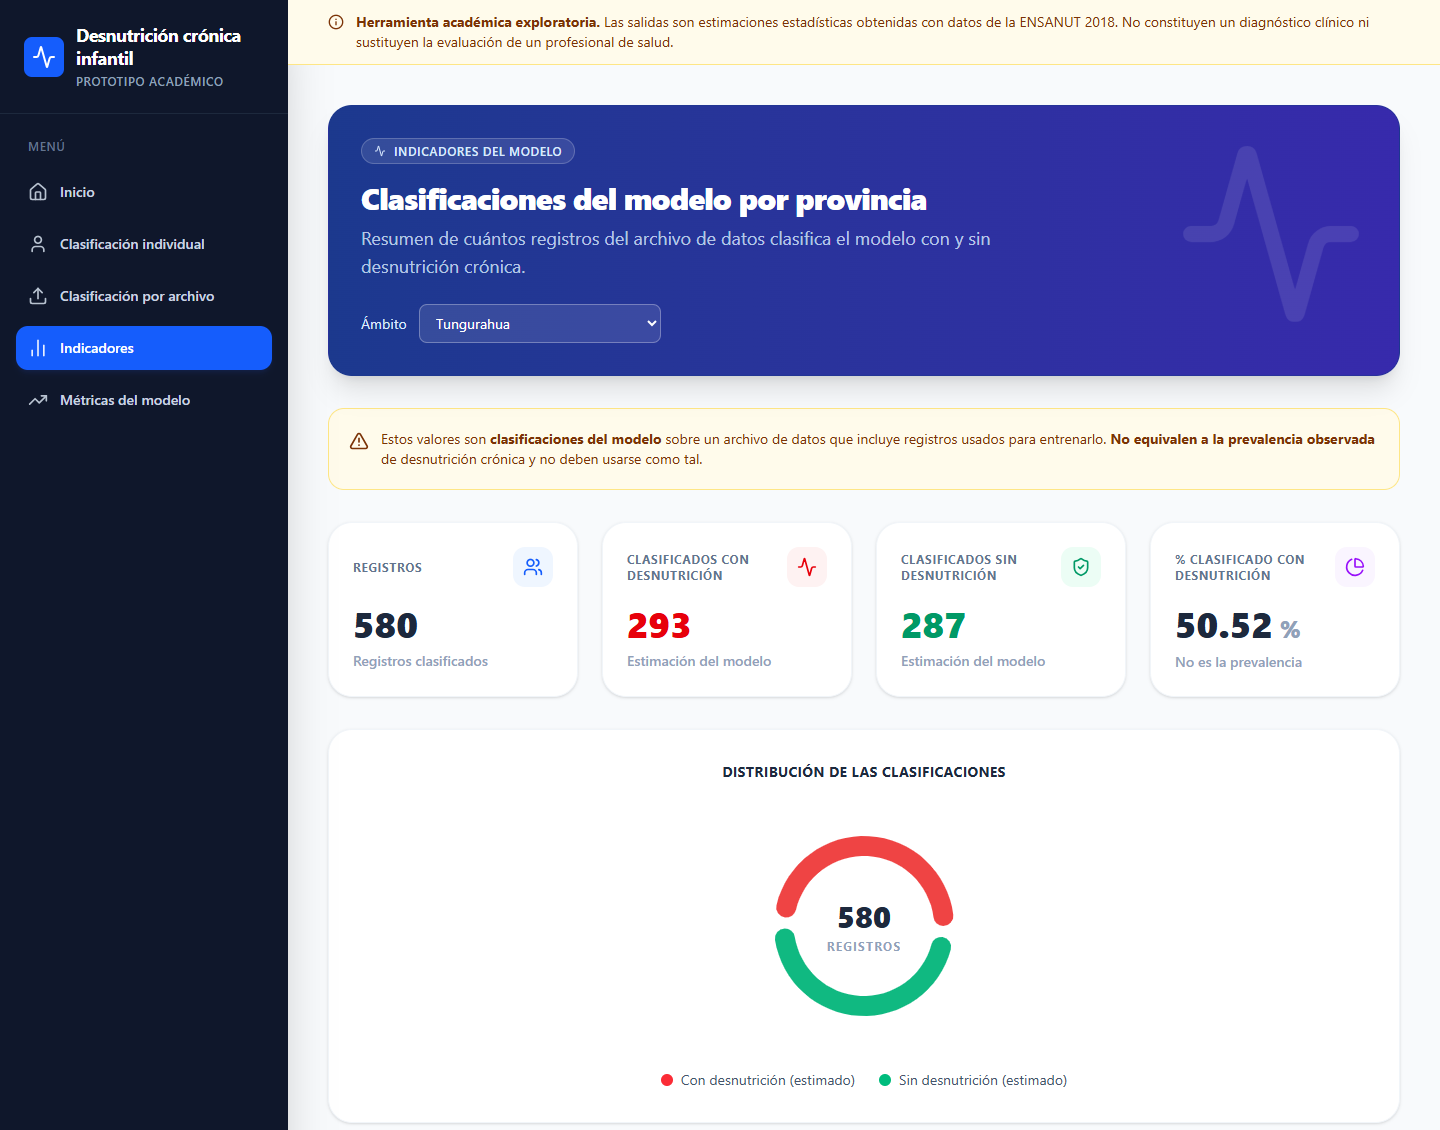
\includegraphics[width=0.85\textwidth]{figuras/ui-dashboard.png}
  \caption{Módulo de indicadores, con el ámbito Tungurahua.}
  \label{fig:ui-dashboard}
\end{figure}

\section*{B.6 Clasificación individual}
El formulario recoge diez datos: edad en meses, sexo, área, provincia, peso y talla al nacer, edad gestacional al nacer, meses de lactancia, y diarrea e infección respiratoria en las dos últimas semanas (Figura~\ref{fig:ui-prediccion}). Las otras 104 variables se envían como nulas y el modelo las completa con la mediana o la moda del entrenamiento. El resultado muestra la clasificación estimada, la puntuación del modelo (no calibrada) y cuántas variables se informaron. \textbf{Uso ilustrativo:} con tan pocos datos la puntuación varía poco (en 512 combinaciones de prueba entre 0.375 y 0.515), por lo que no es interpretable para un niño concreto. Para una clasificación con el modelo evaluado se debe usar la clasificación por archivo.

\begin{figure}[H]
  \centering
  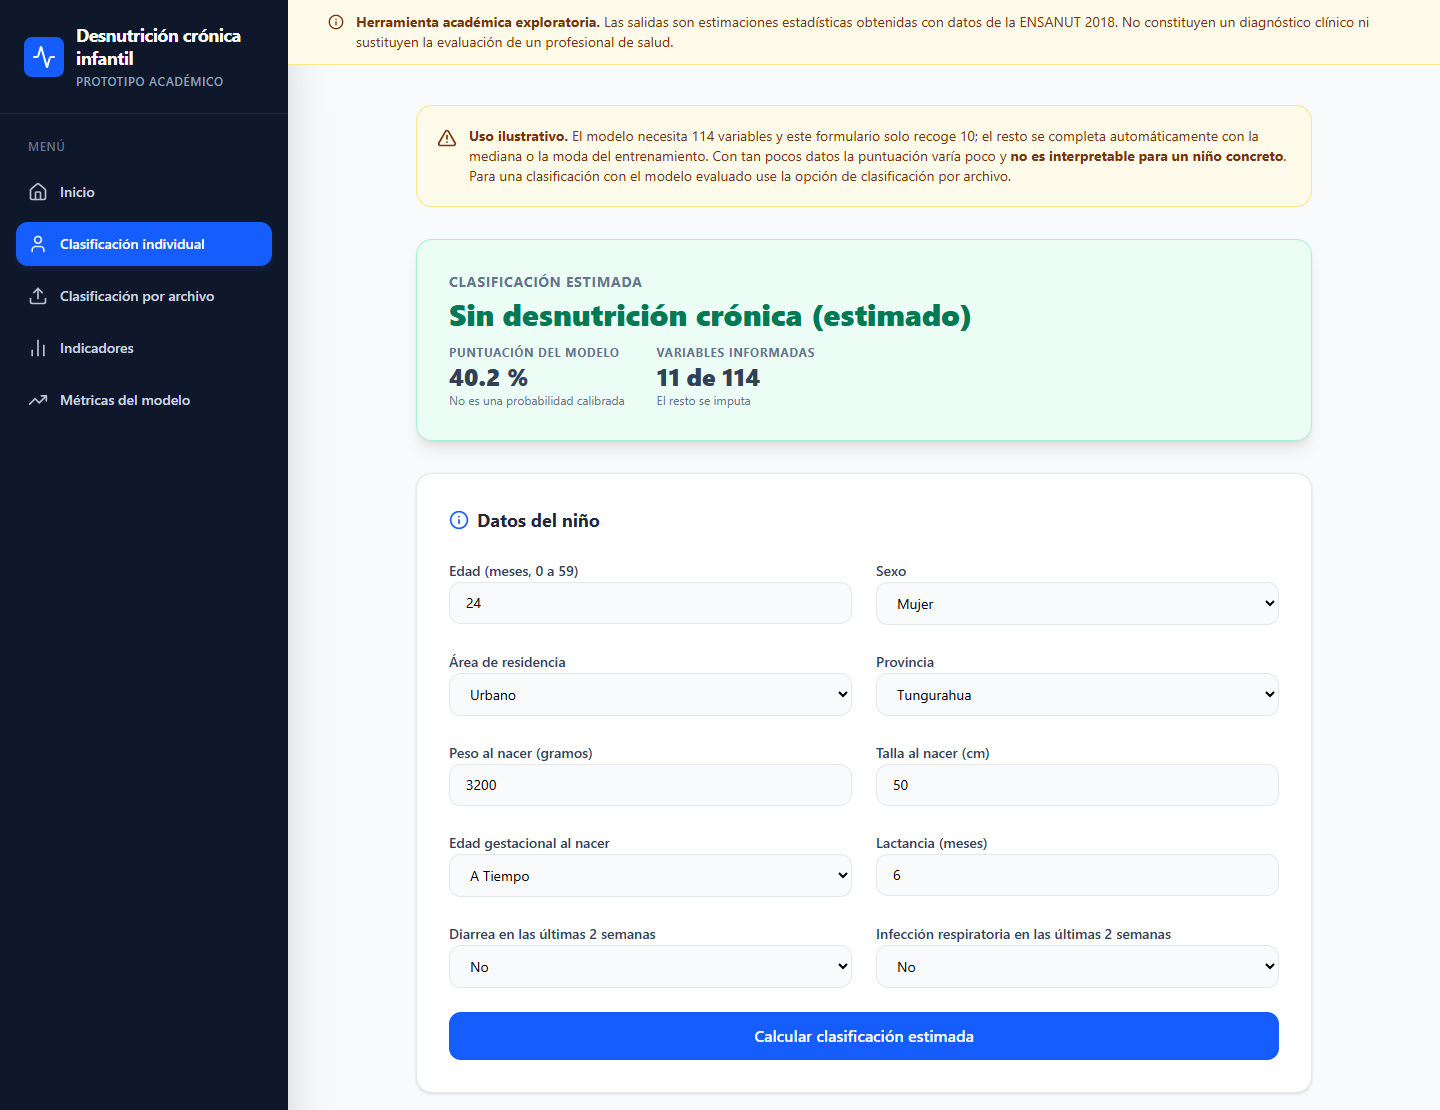
\includegraphics[width=0.85\textwidth]{figuras/ui-prediccion.png}
  \caption{Módulo de clasificación individual con su resultado.}
  \label{fig:ui-prediccion}
\end{figure}

\section*{B.7 Clasificación por archivo}
Pasos (Figura~\ref{fig:ui-masiva}):
\begin{enumerate}
  \item Descargar la plantilla de columnas con el enlace de la pantalla (un CSV solo con el encabezado de las 114 variables).
  \item Completar un niño por fila. Las variables categóricas deben usar las categorías del entrenamiento (Anexo~F).
  \item Seleccionar el archivo (solo formato CSV) y pulsar \textit{Clasificar archivo}.
  \item Se descarga \texttt{resultado\_clasificacion.xlsx} con las columnas originales más \texttt{prediccion} (0 o 1), \texttt{probabilidad} y \texttt{riesgo}.
\end{enumerate}
Si faltan columnas, la pantalla muestra un mensaje y la lista de las faltantes, y no descarga ningún archivo (Figura~\ref{fig:ui-masiva-error}).

\begin{figure}[H]
  \centering
  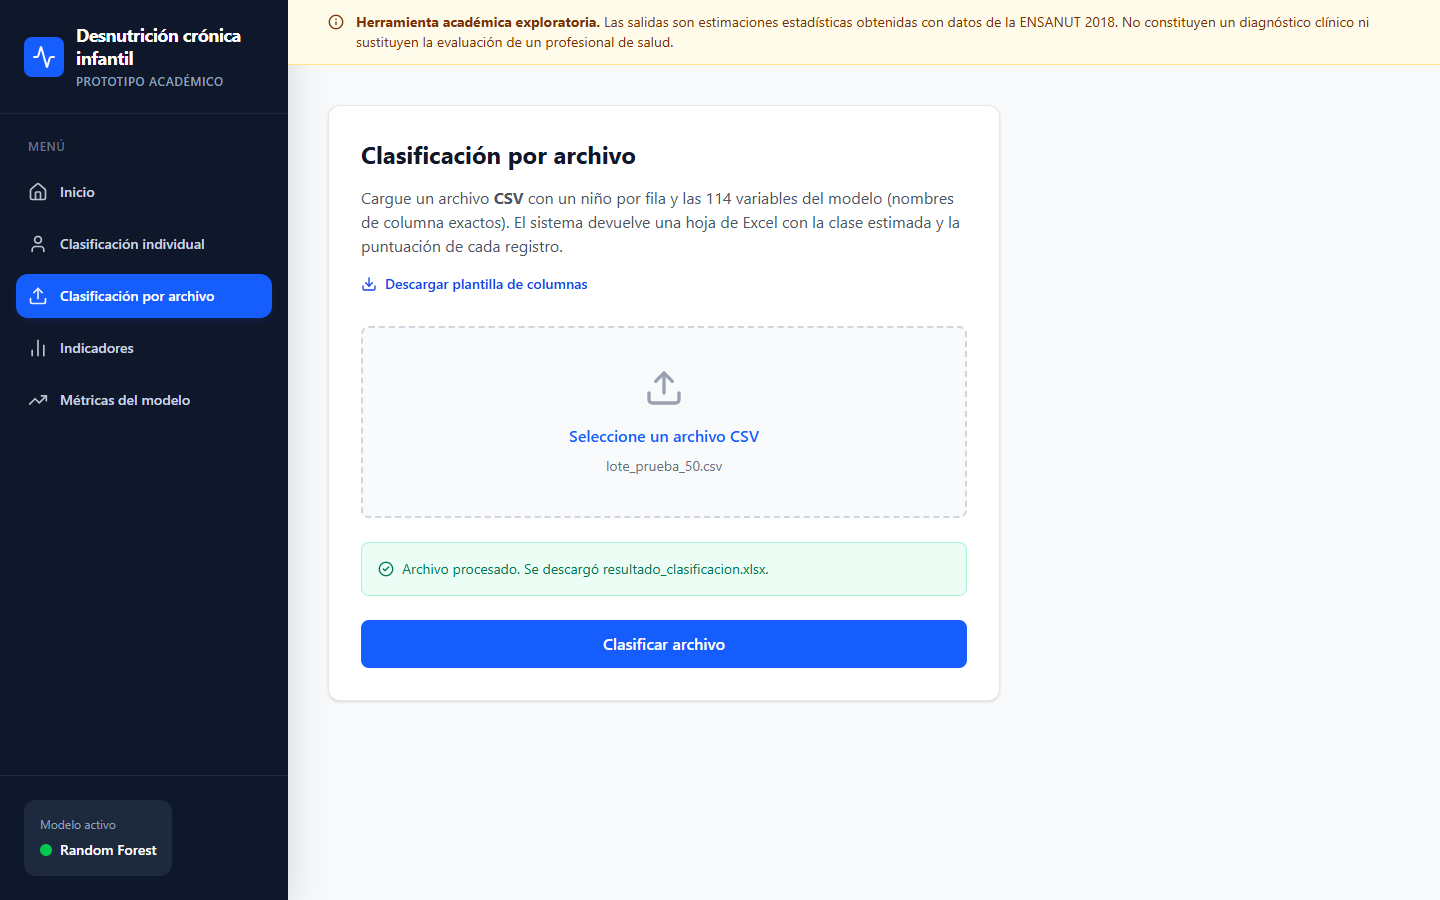
\includegraphics[width=0.85\textwidth]{figuras/ui-masiva.png}
  \caption{Clasificación por archivo: archivo procesado con éxito.}
  \label{fig:ui-masiva}
\end{figure}
\begin{figure}[H]
  \centering
  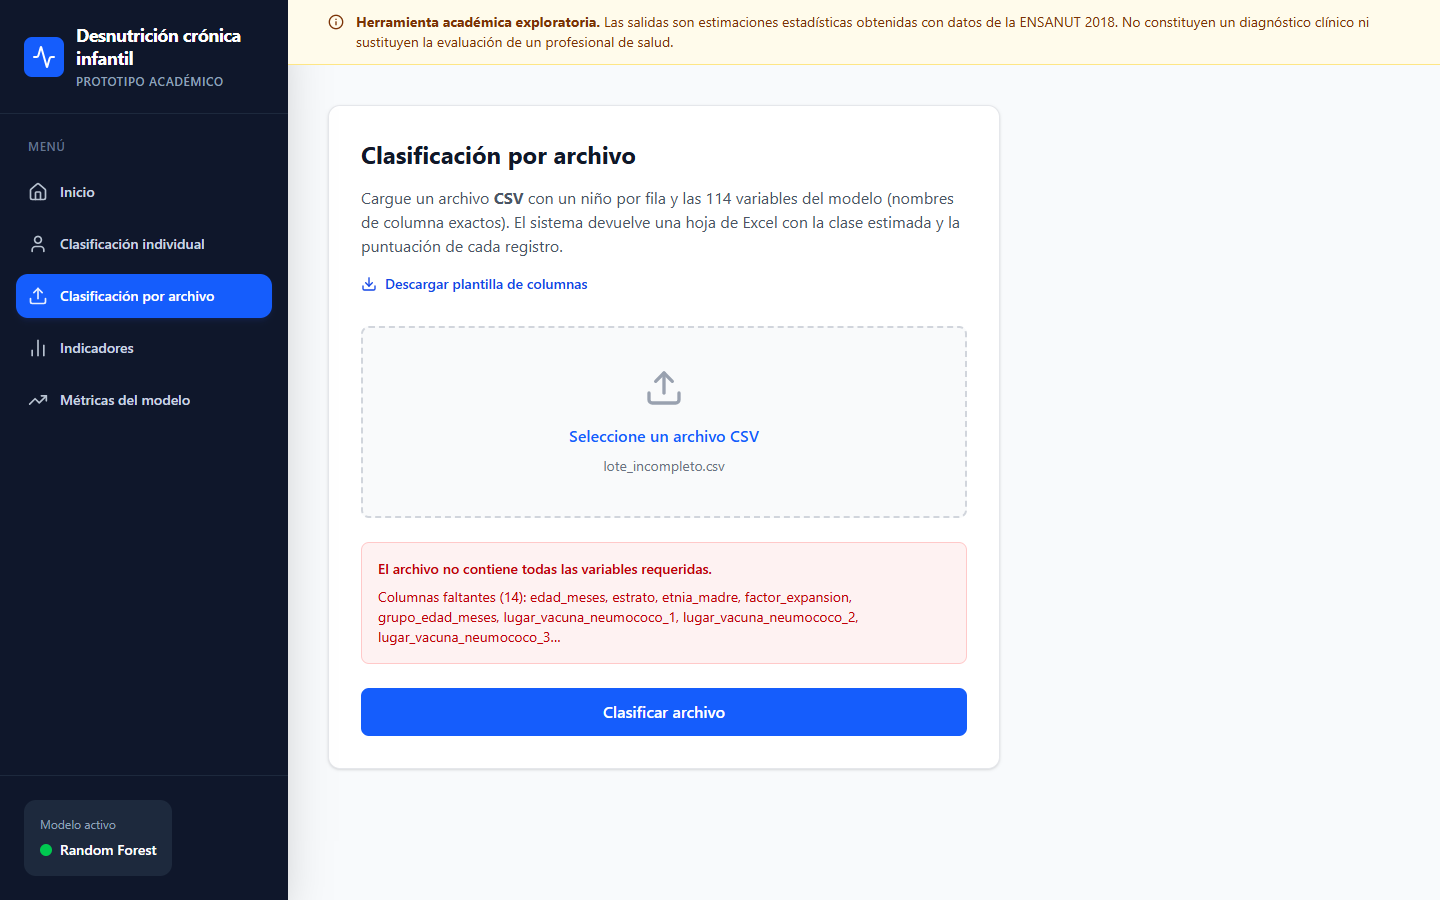
\includegraphics[width=0.85\textwidth]{figuras/ui-masiva-error.png}
  \caption{Clasificación por archivo: mensaje cuando el CSV tiene columnas faltantes.}
  \label{fig:ui-masiva-error}
\end{figure}

\section*{B.8 Métricas del modelo}
Muestra las métricas de la clase con desnutrición crónica en el conjunto de prueba interno (sensibilidad, precisión, F1, exactitud balanceada, ROC-AUC y PR-AUC) y las diez variables más importantes (Figura~\ref{fig:ui-metricas}). Las variables de diseño muestral se marcan en rojo. La importancia no implica causalidad.

\begin{figure}[H]
  \centering
  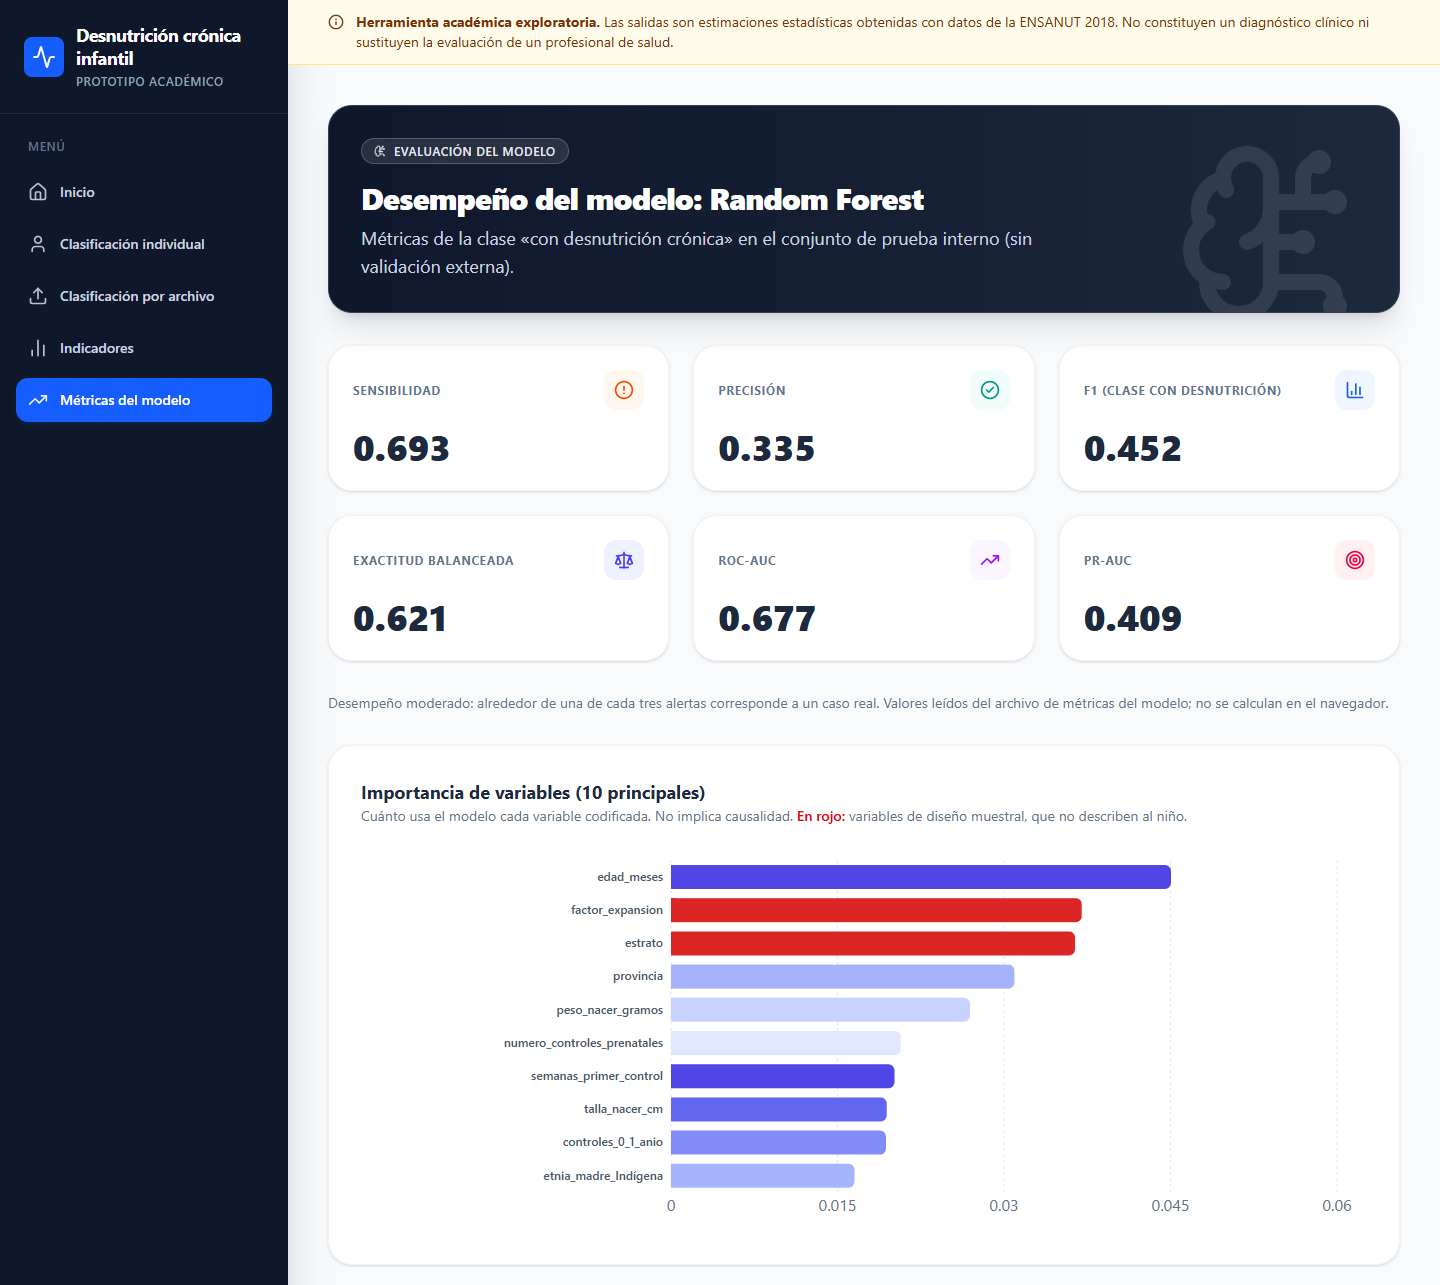
\includegraphics[width=0.85\textwidth]{figuras/ui-metricas.png}
  \caption{Módulo de métricas del modelo.}
  \label{fig:ui-metricas}
\end{figure}

\section*{B.9 Mensajes frecuentes}
\begin{table}[H]
  \caption{Mensajes frecuentes y su causa.}
  \label{tab:mensajes}
  \tablabase\small
  \begin{tabular}{|p{5.0cm}|p{8.4cm}|}
    \hline
    \enc{Mensaje o comportamiento} & \enc{Causa y acción}\\ \hline
    ``El archivo no contiene todas las variables requeridas'' & Faltan columnas en el CSV. Usar la plantilla de columnas\\ \hline
    ``Ocurrió un error al procesar el archivo'' & El archivo no es un CSV válido o tiene categorías no reconocidas. Revisar el formato\\ \hline
    ``API sin conexión'' (barra lateral) & La API no está activa o la dirección configurada es incorrecta\\ \hline
    ``Provincia no válida'' & El ámbito debe elegirse de la lista; la API espera el nombre de la provincia\\ \hline
    Riesgo BAJO con clase estimada positiva (en el Excel) & Ocurría en la versión inicial del servicio; corregido (A.4). Si aparece en un despliegue antiguo, usar la clase\\ \hline
  \end{tabular}
\end{table}

%% ----------------------------------------------------------------- ANEXO C
\anexo{C}{Evidencias de Pruebas del Sistema}

Las pruebas de la API se ejecutaron el 20 de septiembre de 2026 sobre el backend en ejecución local (\textit{TestClient} de FastAPI, modelo v2), con un registro real del conjunto de prueba como entrada. Las pruebas del tablero (CP15 a CP17) se ejecutaron el mismo día en un navegador automatizado (Playwright) sobre la interfaz ya corregida. Además se ejecutaron las 21 pruebas automáticas del repositorio (5 de contrato, 3 del nivel de riesgo, 5 del resumen del tablero y 8 de la lectura de archivos), todas aprobadas.

\begingroup
\scriptsize\setlength{\tabcolsep}{3pt}\arrayrulecolor{black!55}\renewcommand{\arraystretch}{1.1}
\begin{longtable}{|c|p{2.2cm}|p{2.7cm}|p{2.4cm}|p{3.1cm}|c|}
  \caption{Casos de prueba funcional de la API.}
  \label{tab:casos}\\ \hline
  \enc{ID} & \enc{Caso} & \enc{Entrada} & \enc{Esperado} & \enc{Obtenido} & \enc{Estado}\\ \hline
  \endfirsthead
  \tablacont{6}\hline
  \enc{ID} & \enc{Caso} & \enc{Entrada} & \enc{Esperado} & \enc{Obtenido} & \enc{Estado}\\ \hline
  \endhead
  \hline\endfoot
  CP1 & Estado del servicio & \texttt{GET /health} & HTTP 200 y \texttt{OK} & HTTP 200, \texttt{\{"status":"OK"\}} & Pasa\\ \hline
  CP2 & Variables del modelo & \texttt{GET /features} & 114 variables & HTTP 200, 114 variables & Pasa\\ \hline
  CP3 & Información de la API & \texttt{GET /info} & HTTP 200 y modelo activo & HTTP 200, modelo Random Forest & Pasa\\ \hline
  CP4 & Predicción individual & \texttt{POST /predict} con 114 variables & HTTP 200; clase, probabilidad en [0,1] y riesgo & HTTP 200; clase 1, probabilidad 0.437, riesgo MEDIO & Pasa (ver nota)\\ \hline
  CP5 & Variable faltante & \texttt{POST /predict} con 113 variables & HTTP 400 & HTTP 400 & Pasa\\ \hline
  CP6 & Variable sobrante & \texttt{POST /predict} con 115 variables & HTTP 400 & HTTP 400 & Pasa\\ \hline
  CP7 & Cuerpo vacío & \texttt{POST /predict} con \texttt{\{\}} & HTTP 400 & HTTP 400 & Pasa\\ \hline
  CP8 & Predicción masiva & \texttt{POST /predict-file}, CSV de 50 registros & Archivo \texttt{.xlsx} de 50 filas & HTTP 200; \texttt{.xlsx} de 50 filas & Pasa\\ \hline
  CP9 & Resumen nacional & \texttt{GET /dashboard} & HTTP 200 con totales del conjunto de prueba & HTTP 200; \num{3699} registros; 912 observados; \num{1887} clasificados (sensibilidad 0.693) & Pasa (ver nota)\\ \hline
  CP10 & Resumen por provincia & \texttt{GET /dashboard} con provincia Tungurahua & HTTP 200 con totales del conjunto de prueba & HTTP 200; 112 registros; 35 observados; 57 clasificados (sensibilidad 0.686) & Pasa (ver nota)\\ \hline
  CP11 & Métricas del modelo & \texttt{GET /dashboard/}\allowbreak\texttt{metricas} & Valores de \texttt{metricas\_v2.json} & HTTP 200; valores idénticos & Pasa\\ \hline
  CP12 & Importancia de variables & \texttt{GET /dashboard/}\allowbreak\texttt{importancia} & HTTP 200 con lista & HTTP 200; lista de variables & Pasa\\ \hline
  CP13 & Documentación & \texttt{GET /docs} & HTTP 200 & HTTP 200 & Pasa\\ \hline
  CP14 & Archivo Excel en predicción masiva & \texttt{POST /predict-file} con un \texttt{.xlsx} & Resultado o mensaje de error controlado & HTTP 200; \texttt{.xlsx} de 50 filas. Un Excel dañado, un \texttt{.xls} o un archivo vacío devuelven un mensaje de error & Pasa (ver nota)\\ \hline
  CP15 & Formulario individual & 512 combinaciones de los 10 datos, resto nulo (formulario corregido) & Probabilidades que varíen según los datos & Entre 0.375 y 0.515; \SI{85.5}{\percent} con clase 1 (la versión inicial: 0.436--0.512, todas con clase 1) & Falla\\ \hline
  CP16 & Tablero: CSV incompleto & CSV de 5 registros con 100 de 114 columnas & Mensaje claro con columnas faltantes; sin descarga & Mensaje con las columnas faltantes; sin descarga & Pasa\\ \hline
  CP17 & Tablero: CSV válido & CSV de 50 registros del conjunto de prueba & Descarga de \texttt{.xlsx} de 50 filas & \texttt{resultado\_clasificacion.xlsx} con 50 filas y columnas \texttt{prediccion}, \texttt{probabilidad} y \texttt{riesgo} & Pasa\\ \hline
\end{longtable}
\endgroup

\noindent\textbf{Notas.} En CP4, con la versión evaluada inicialmente, la clase asignada (1) y el riesgo (BAJO) no coincidían porque usaban cortes distintos; tras alinear el riesgo con el umbral de 0.42 el caso se volvió a ejecutar y devuelve riesgo MEDIO. Con el servicio corregido, los 50 registros de CP17 son consistentes: 25 con riesgo BAJO (todos clase 0), 21 MEDIO y 4 ALTO (todos clase 1). En la versión evaluada inicialmente, CP9 y CP10 devolvían positivos predichos por el modelo sobre un archivo que incluía los datos de entrenamiento (\num{20510} registros y \num{10626} casos predichos a nivel nacional; 580 registros y 293 casos en Tungurahua), no casos observados. El servicio se corrigió para usar el conjunto de prueba y ambos casos se volvieron a ejecutar: los valores de la tabla son los del servicio corregido y reproducen las métricas de \texttt{metricas\_v2.json} (sensibilidad 0.693 y precisión 0.335). CP14 y CP15 se agregaron al descubrir el comportamiento del servicio de archivos y del formulario. En la versión evaluada inicialmente, CP14 producía una excepción no controlada (\texttt{UnicodeDecodeError}) porque el servicio leía el Excel como CSV; se corrigió (lectura de \texttt{.xlsx} y mensajes de error controlados) y el caso se volvió a ejecutar; CP16 y CP17 verifican la carga de archivos del tablero corregido (Anexo~B).

\noindent\textbf{Resumen.} De los 17 casos, 16 pasan y 1 falla (CP15). Los casos CP1 a CP13 verifican el contrato de la API con datos completos; CP14 verifica el servicio de archivos con Excel (falló en la versión inicial y pasa con el servicio corregido) y CP15 muestra la escasa variación del formulario individual.

\noindent\textbf{Latencia de \texttt{POST /predict}} (100 solicitudes, ejecución local sin red): mediana de 29 ms, percentil 95 de 33 ms y máximo de 38 ms.

\section*{C.1 Ejemplo de solicitud y respuesta (CP4)}
\begin{lstlisting}[frame=single,basicstyle=\ttfamily\footnotesize]
Entrada: registro 0 del conjunto de prueba (114 variables)
Salida : {"prediccion": 1,
          "descripcion": "Con desnutrición crónica",
          "probabilidad": 0.437,
          "riesgo": "MEDIO"}
Cálculo directo sobre el modelo (sin API): 0.437
\end{lstlisting}

\section*{C.2 Pruebas automáticas del repositorio}
\begin{lstlisting}[frame=single,basicstyle=\ttfamily\footnotesize]
$ python -m pytest -q tests
.....................                           [100%]
21 passed
\end{lstlisting}

%% ----------------------------------------------------------------- ANEXO D
\anexo{D}{Trazabilidad entre Objetivos, Métodos y Resultados}

\begin{table}[H]
  \caption{Matriz de trazabilidad.}
  \label{tab:traza}
  \tablabase\scriptsize
  \begin{tabular}{|p{2.6cm}|p{3.1cm}|p{3.6cm}|p{3.5cm}|}
    \hline
    \enc{Objetivo específico} & \enc{Método (capítulo II)} & \enc{Resultado (capítulo III)} & \enc{Conclusión (capítulo IV)}\\ \hline
    1. Analizar y preparar los datos & Fases Obtener, Limpiar y Explorar (Tabla~\ref{tab:osemn}) & Tabla~\ref{tab:datos}; corrección de v1 (Tabla~\ref{tab:v1v2}) & Objetivo 1\\ \hline
    2. Diseñar arquitectura y protocolo & Diseño y requerimientos (Tablas~\ref{tab:rf}, \ref{tab:rnf}) & Tabla~\ref{tab:experimento} & Objetivo 2\\ \hline
    3. Entrenar, comparar y evaluar & Protocolo experimental y métricas & Tablas~\ref{tab:metricas}, \ref{tab:tung}, \ref{tab:sobreajuste}; Figuras~\ref{fig:comparacion}, \ref{fig:matriz}, \ref{fig:curvas} & Objetivo 3\\ \hline
    4. Implementar API y tablero & Contrato de la API (Tabla~\ref{tab:api}) & Tabla~\ref{tab:stack}; Anexos A y B & Objetivo 4\\ \hline
    5. Validar y documentar limitaciones & Pruebas funcionales (Tabla~\ref{tab:tecnicas}) & Anexo C; Tabla~\ref{tab:cumplimiento} & Objetivo 5 y limitaciones\\ \hline
  \end{tabular}
\end{table}

\begin{table}[H]
  \caption{Requerimientos y casos de prueba que los verifican.}
  \label{tab:req-cp}
  \tablabase\small
  \begin{tabular}{|c|p{5.2cm}|p{5.2cm}|}
    \hline
    \enc{Requerimiento} & \enc{Evidencia principal} & \enc{Casos de prueba}\\ \hline
    RF3, RNF1 & Servicio de predicción y validación de entradas & CP4, CP5, CP6, CP7\\ \hline
    RF4 & Predicción masiva & CP8, CP14, CP16, CP17\\ \hline
    RF5 & Métricas del modelo & CP11\\ \hline
    RF6 & Indicadores del tablero & CP9, CP10, CP12\\ \hline
    RF7 & Documentación interactiva & CP13\\ \hline
    RNF2 & Rendimiento & Latencia de 100 solicitudes\\ \hline
    RNF3 & Disponibilidad & CP1, CP3\\ \hline
    RNF7 & Uso responsable & Revisión de la interfaz en todas las pantallas (Anexo~B)\\ \hline
  \end{tabular}
\end{table}

%% ----------------------------------------------------------------- ANEXO E
\anexo{E}{Repositorio de Versionamiento de Código}

\section*{E.1 Repositorios}
El código está en un único repositorio consolidado de GitHub, cuya cuenta propietaria es \texttt{8afer99c}: \url{https://github.com/8afer99c/desnutricion_tesis}. Contiene los notebooks originales, el pipeline corregido (\texttt{pipeline\_v2}), la API y el tablero. Se publicaron dos ramas: \texttt{pipeline-v2-fixes} (rama por defecto del repositorio) y \texttt{main} (rama desplegada). El historial de commits conserva la autoría que Git registró en cada commit.

La versión final del tablero corresponde al commit \texttt{b441664} de \texttt{pipeline-v2-fixes} y a su integración en \texttt{main} (commit \texttt{8df0ade}, 20 de septiembre de 2026). El archivo \texttt{metricas\_v2.json} se versionó en \texttt{45928dd} (\texttt{main}) y \texttt{af4fcf4} (\texttt{pipeline-v2-fixes}), y la corrección del nivel de riesgo de la API está en \texttt{588d8fe} (\texttt{main}) y \texttt{7b37205} (\texttt{pipeline-v2-fixes}). El resumen del tablero con el conjunto de prueba (\texttt{data/test\_v2.csv}) está en \texttt{edf40ae} (\texttt{main}) y \texttt{d785b95} (\texttt{pipeline-v2-fixes}). La lectura controlada de CSV y Excel en \texttt{/predict-file} está en \texttt{89a23d5} (\texttt{main}) y \texttt{db5a77f} (\texttt{pipeline-v2-fixes}). Los notebooks y el paquete \texttt{pipeline\_v2} se conservan en el historial hasta el commit \texttt{1b4b767}, ya que desde el commit \texttt{bf27226} la reorganización del repositorio los retiró del árbol de archivos actual; se recuperan con \texttt{git show <commit>:<ruta>}.

\section*{E.2 Reproducción de los resultados}
Desde la carpeta del proyecto, con Python 3.13 y las versiones de la Tabla~\ref{tab:deps}, el pipeline se ejecuta en este orden:
\begin{lstlisting}[frame=single,basicstyle=\ttfamily\footnotesize]
python -m pipeline_v2.build_clean_dataset   # base sin fuga (18 493)
python -m pipeline_v2.split_dataset         # train_v2 / test_v2
python -m pipeline_v2.leakage_screen        # revision de fuga
python -m pipeline_v2.entrenar_modelo       # modelo_v2 y metricas_v2
python -m pipeline_v2.comparar_v1_v2        # comparacion v1 vs v2
python -m pipeline_v2.tabla_experimento     # tabla unica del experimento
\end{lstlisting}
Los archivos generados quedan en \texttt{pipeline\_v2/output}. Cargar \texttt{modelo\_v2.joblib} requiere la misma versión de scikit-learn con la que se entrenó (1.6.1).

\section*{E.3 Historial de cambios del pipeline corregido}
\begingroup
\scriptsize\setlength{\tabcolsep}{3pt}\arrayrulecolor{black!55}\renewcommand{\arraystretch}{1.1}
\begin{longtable}{|c|c|p{9.8cm}|}
  \caption{Commits principales del repositorio (ramas \texttt{pipeline-v2-fixes} y \texttt{main}).}
  \label{tab:commits}\\ \hline
  \enc{Fecha} & \enc{Commit} & \enc{Descripción}\\ \hline
  \endfirsthead
  \tablacont{3}\hline
  \enc{Fecha} & \enc{Commit} & \enc{Descripción}\\ \hline
  \endhead
  \hline\endfoot
  2026-09-12 & \texttt{7cc7372} & Estructura del paquete \texttt{pipeline\_v2} y entorno de desarrollo\\ \hline
  2026-09-12 & \texttt{46c702d} & Captura de las métricas base del modelo v1\\ \hline
  2026-09-12 & \texttt{b00adf2} & Eliminar filas con variable objetivo sin medir en vez de imputarlas\\ \hline
  2026-09-12 & \texttt{b873079} & Regenerar la partición entrenamiento/prueba limpia y reproducible\\ \hline
  2026-09-12 & \texttt{d711dab} & Revisión automática de fuga por variable\\ \hline
  2026-09-13 & \texttt{2a744f9} & Pipeline de entrenamiento: selección real, desbalance, umbral y métricas por clase\\ \hline
  2026-09-13 & \texttt{f405ca5} & Comparación controlada entre v1 y v2\\ \hline
  2026-09-13 & \texttt{c03200d} & Reportar sobreajuste e hiperparámetros; aislar el preprocesador\\ \hline
  2026-09-13 & \texttt{54cd860} & Aviso sobre los números inflados de v1 y tabla del experimento\\ \hline
  2026-09-13 & \texttt{20f4bde} & Regularizar Random Forest (menor tamaño y sobreajuste)\\ \hline
  2026-09-13 & \texttt{1b4b767} & Incorporar el código de la API y los notebooks al repositorio consolidado\\ \hline
  2026-09-13 & \texttt{bf27226} & Interfaz web y arquitectura estructurada\\ \hline
  2026-09-13 & \texttt{1da04ff} & Variable \texttt{VITE\_API\_URL} para el despliegue en Vercel\\ \hline
  2026-09-20 & \texttt{b441664} & Interfaz académica exploratoria: aviso, métricas v2, formulario con 114 variables y carga CSV corregidos\\ \hline
  2026-09-20 & \texttt{8df0ade} & Integración de \texttt{pipeline-v2-fixes} en \texttt{main} y recompilación de la aplicación web (rama \texttt{main})\\ \hline
  2026-09-20 & \texttt{45928dd}, \texttt{af4fcf4} & Versionar \texttt{metricas\_v2.json} (umbral 0.42 y métricas del modelo v2 en el despliegue)\\ \hline
  2026-09-20 & \texttt{588d8fe}, \texttt{7b37205} & Nivel de riesgo de la API coherente con el umbral de decisión 0.42 (\texttt{main} y \texttt{pipeline-v2-fixes})\\ \hline
  2026-09-20 & \texttt{edf40ae}, \texttt{d785b95} & Resumen del tablero con el conjunto de prueba: casos observados y clasificados, sensibilidad y precisión\\ \hline
  2026-09-20 & \texttt{89a23d5}, \texttt{db5a77f} & Lectura controlada de CSV y Excel en \texttt{/predict-file}, con mensajes de error para archivos inválidos\\ \hline
\end{longtable}
\endgroup

%% ----------------------------------------------------------------- ANEXO F
\anexo{F}{Diccionario de las Variables Predictoras}

La Tabla~\ref{tab:diccionario} describe las 114 variables predictoras en el orden de las columnas del conjunto de datos: tipo, porcentaje de valores ausentes en la base original, rango o categorías principales y etiqueta de la pregunta original de la ENSANUT. La variable objetivo es \texttt{desnutricion\_cronica}. Las categorías se muestran tal como figuran en los datos.

\begingroup
\tiny\setlength{\tabcolsep}{2.5pt}\arrayrulecolor{black!55}\renewcommand{\arraystretch}{1.1}
\begin{longtable}{|r|p{3.1cm}|c|r|p{3.0cm}|p{3.8cm}|}
  \caption{Diccionario de las variables predictoras. \% nulos: porcentaje de valores ausentes en la base original antes de la imputación.}
  \label{tab:diccionario}\\ \hline
  \enc{N.º} & \enc{Variable} & \enc{Tipo} & \enc{\% nulos} & \enc{Rango o categorías} & \enc{Etiqueta original (ENSANUT)} \\ \hline
  \endfirsthead
  \tablacont{6}\hline
  \enc{N.º} & \enc{Variable} & \enc{Tipo} & \enc{\% nulos} & \enc{Rango o categorías} & \enc{Etiqueta original (ENSANUT)} \\ \hline
  \endhead
  \hline\endfoot
  1 & \texttt{area} & Cat. & 0.0 & 2 cat.: Urbano; Rural & Área \\ \hline
  2 & \texttt{provincia} & Num. & 0.0 & 1 a 90 & Provincia \\ \hline
  3 & \texttt{orden\_hijo} & Num. & 0.0 & 1 a 3 & Orden del hijo \\ \hline
  4 & \texttt{sexo} & Cat. & 0.0 & 2 cat.: Hombre; Mujer & Sexo \\ \hline
  5 & \texttt{embarazo\_planeado} & Cat. & 0.0 & 4 cat.: Tener Ese Hijo?; Quería Esperar Mas T; … & 403.  En la época en la que quedó embarazada de (…), quería U… \\ \hline
  6 & \texttt{embarazo\_deseado\_pareja} & Cat. & 0.0 & 4 cat.: Tener Ese Hijo?; Quería Esperar Mas T; … & 405.  ¿Quería su pareja: \\ \hline
  7 & \texttt{control\_prenatal} & Cat. & 0.0 & 2 cat.: Si; No & 406.  ¿Tuvo algún control prenatal cuando estaba embarazada d… \\ \hline
  8 & \texttt{lugar\_control\_prenatal} & Cat. & 4.2 & 10 cat.: Establecimientos De ; Clínica/Consultorio ; … & 407.a ¿Dónde se hizo el control con mayor frecuencia? \\ \hline
  9 & \texttt{consumo\_micronutrientes\_embarazo} & Cat. & 4.2 & 4 cat.: Hierro Más Ácido Fól; Hierro?; … & 408.  ¿Consumió algún micronutriente durante el embarazo como: \\ \hline
  10 & \texttt{frecuencia\_micronutrientes} & Cat. & 6.3 & 3 cat.: Diaria; Pasando Un Día; … & 409.a ¿Con qué frecuencia tomaba Los micronutrientes? \\ \hline
  11 & \texttt{control\_peso\_embarazo} & Cat. & 4.2 & 3 cat.: Si; No; … & 410.  ¿Durante el embarazo le pesaron? \\ \hline
  12 & \texttt{medicion\_altura\_uterina} & Cat. & 4.2 & 3 cat.: Si; No; … & 411.  ¿Durante el embarazo le midieron la barriga? \\ \hline
  13 & \texttt{examen\_vih\_embarazo} & Cat. & 4.2 & 3 cat.: Si; No; … & 412.a ¿Durante el embarazo le hicieron un examen de VIH? \\ \hline
  14 & \texttt{numero\_examenes\_vih} & Num. & 13.3 & 1 a 88 & 412.b Cuántos? \\ \hline
  15 & \texttt{control\_presion\_embarazo} & Cat. & 4.2 & 3 cat.: Si; No; … & 413.  ¿Durante el embarazo ¿le tomaron la presión? \\ \hline
  16 & \texttt{examen\_sangre\_embarazo} & Cat. & 4.2 & 3 cat.: Si; No; … & 414.  ¿Durante el embarazo ¿hicieron un examen de sangre? \\ \hline
  17 & \texttt{examen\_orina\_embarazo} & Cat. & 4.2 & 3 cat.: Si; No; … & 415.  ¿Durante el embarazo ¿hicieron un examen de orina? \\ \hline
  18 & \texttt{examen\_sifilis\_embarazo} & Cat. & 4.2 & 3 cat.: Si; No Sabe / No Respond; … & 416.  ¿Durante el embarazo ¿hicieron un examen de sífilis? \\ \hline
  19 & \texttt{vacuna\_tetanos} & Cat. & 4.2 & 3 cat.: Si; No; … & 417.  ¿Durante el embarazo ¿le vacunaron contra el tétanos? \\ \hline
  20 & \texttt{dosis\_tetanos} & Num. & 13.6 & 1 a 99 & 418.  ¿Cuántas veces le vacunaron contra el tétanos? \\ \hline
  21 & \texttt{consejeria\_embarazo} & Cat. & 4.2 & 3 cat.: Si; No; … & 419.a ¿Durante el control del embarazo, recibió consejería o … \\ \hline
  22 & \texttt{consejeria\_micronutrientes} & Cat. & 4.2 & 3 cat.: Si; No; … & 419.b Uso de micronutrientes (hierro, ácido fólico)? \\ \hline
  23 & \texttt{consejeria\_signos\_alarma} & Cat. & 4.2 & 3 cat.: Si; No; … & 419.c Signos de alarma del embarazo (sangrado vaginal, falta … \\ \hline
  24 & \texttt{consejeria\_higiene\_alimentos} & Cat. & 4.2 & 3 cat.: Si; No; … & 419.d Higiene en preparación de alimentos? \\ \hline
  25 & \texttt{consejeria\_lavado\_manos} & Cat. & 4.2 & 3 cat.: Si; No; … & 419.e Lavado de manos? \\ \hline
  26 & \texttt{consejeria\_anticonceptivos} & Cat. & 4.2 & 3 cat.: Si; No; … & 419.f Métodos anticonceptivos? \\ \hline
  27 & \texttt{consejeria\_apego\_lactancia} & Cat. & 4.2 & 3 cat.: Si; No; … & 419.g El apego inmediato, lactancia en la primera hora de vid… \\ \hline
  28 & \texttt{semanas\_primer\_control} & Num. & 4.2 & 0 a 40 & 420.  ¿Cuántas semanas de embarazo tenía cuando le hicieron e… \\ \hline
  29 & \texttt{numero\_controles\_prenatales} & Num. & 4.2 & 0 a 88 & 421.  En total, ¿cuántos controles tuvo antes del parto? \\ \hline
  30 & \texttt{lugar\_parto} & Cat. & 0.0 & 9 cat.: Establecimientos De ; Clínica/Consultorio ; … & 423.a ¿En que lugar tuvo el parto de (..).? \\ \hline
  31 & \texttt{personal\_parto} & Cat. & 0.0 & 8 cat.: Médico; Obstetriz; … & 424.  ¿Qué persona ó profesional le tendió? \\ \hline
  32 & \texttt{tipo\_parto} & Cat. & 0.0 & 2 cat.: Normal (Vaginal); Césaria & 425.  El parto de (...) fue: \\ \hline
  33 & \texttt{prematuro} & Cat. & 0.0 & 4 cat.: A Tiempo; Prematuro; … & 426.  ¿El nacimiento de (...) fue a los 9 meses o antes de ti… \\ \hline
  34 & \texttt{peso\_registrado\_nacer} & Cat. & 0.0 & 2 cat.: Si; No & 428.  ¿Le pesaron a (…) en el momento de nacer o en los prime… \\ \hline
  35 & \texttt{tamizaje\_neonatal} & Cat. & 0.0 & 2 cat.: Si; No & 429.  ¿Le Realizaron a (…) La prueba del Tamizaje Neonatal (p… \\ \hline
  36 & \texttt{bano\_antes\_24h} & Cat. & 0.0 & 3 cat.: Si; No; … & 430.  ¿Le bañaron a (…) antes de cumplir 24 horas de su nacim… \\ \hline
  37 & \texttt{corte\_oportuno\_cordon} & Cat. & 0.0 & 3 cat.: Si; No sabe; … & 431.  ¿Esperaron al menos un minuto para realizar el corte de… \\ \hline
  38 & \texttt{carne\_salud\_infantil} & Cat. & 0.0 & 3 cat.: Si; Si Le Entregaron Per; … & 432.  Tiene usted el carné de salud infantil o libreta integr… \\ \hline
  39 & \texttt{registro\_curva\_crecimiento} & Cat. & 37.8 & 2 cat.: No; Si & 433.a ENCUESTADOR/A OBSERVE SI EL CARNÉ REGISTRA PUNTOS EN LA… \\ \hline
  40 & \texttt{registro\_talla\_nacer} & Cat. & 37.8 & 2 cat.: Si; No & 434.a ENCUESTADOR/A OBSERVE SI EL CARNÉ REGISTRA: TALLA AL NACER \\ \hline
  41 & \texttt{talla\_nacer\_cm} & Num. & 57.3 & 0.42 a 5000 & 434.b cm \\ \hline
  42 & \texttt{registro\_perimetro\_cefalico} & Cat. & 37.8 & 2 cat.: Si; No & 435.a ENCUESTADOR/A OBSERVE SI EL CARNÉ REGISTRA PERÍMETRO CE… \\ \hline
  43 & \texttt{perimetro\_cefalico\_cm} & Num. & 62.8 & 1 a 2603 & 435.b cm \\ \hline
  44 & \texttt{registro\_peso\_nacer} & Cat. & 37.8 & 2 cat.: Si; No & 436.a ENCUESTADOR/A OBSERVE SI EL CARNÉ REGISTRA:PESO AL NACER \\ \hline
  45 & \texttt{peso\_nacer\_gramos} & Num. & 56.1 & 7 a 9800 & 436.b gramos \\ \hline
  46 & \texttt{peso\_nacer\_reportado} & Cat. & 43.9 & 4 cat.: No sabe; Gramos; … & 437.a ¿Cuánto pesó (…)? \\ \hline
  47 & \texttt{bajo\_peso\_nacer} & Cat. & 63.8 & 3 cat.: No sabe; No; … & 438.  ¿(…) Peso menos de 5.5 Libras, 2.5 Kilogramos o 2500 gr… \\ \hline
  48 & \texttt{tamano\_recien\_nacido} & Cat. & 0.0 & 5 cat.: Igual; Más Grande; … & 439.  En comparación con otros niños recién nacidos, ¿cómo co… \\ \hline
  49 & \texttt{control\_posparto} & Cat. & 0.0 & 2 cat.: Si; No & 440.  ¿Tuvo usted algún control después del parto de (...)? \\ \hline
  50 & \texttt{tiempo\_primer\_control\_posparto} & Num. & 38.3 & 0 a 45 & 441.a ¿Cuánto tiempo después del parto de (...) tuvo su prime… \\ \hline
  51 & \texttt{lugar\_control\_posparto} & Cat. & 38.3 & 10 cat.: Establecimientos De ; Clínica/Consultorio ; … & 442.  ¿Dónde tuvo el control de post parto? \\ \hline
  52 & \texttt{control\_medico\_nino} & Cat. & 0.0 & 2 cat.: Si; No & 448.  ¿Después de que nació (...), le llevó para control médico? \\ \hline
  53 & \texttt{tiempo\_primer\_control\_nino} & Num. & 4.1 & 0 a 77 & 449.  ¿Qué tiempo después de nacido (…), le llevó al control … \\ \hline
  54 & \texttt{motivo\_control\_nino} & Cat. & 4.1 & 3 cat.: ¿Para Control Niño S; ¿Estaba Enfermo?; … & 450.  ¿Porqué o para qué le llevó a (…): \\ \hline
  55 & \texttt{controles\_0\_1\_anio} & Num. & 16.6 & 0 a 88 & 451.a ¿De 0 a menos de 1 años ? \\ \hline
  56 & \texttt{controles\_1\_2\_anios} & Num. & 16.6 & 0 a 88 & 451.b ¿De 1 año a menos de 2 años ? \\ \hline
  57 & \texttt{controles\_2\_5\_anios} & Num. & 16.6 & 0 a 99 & 451.c ¿De 2 años a menos de 5 años ? \\ \hline
  58 & \texttt{numero\_controles\_carnet} & Num. & 16.6 & 0 a 24 & 451.a N° de controles en el carnet Último nacido vivo \\ \hline
  59 & \texttt{establecimiento\_salud} & Cat. & 4.1 & 10 cat.: Establecimientos De ; Clínica/Consultorio ; … & 452.  ¿A qué establecimiento o proveedor de salud llevó a (…)? \\ \hline
  60 & \texttt{consejeria\_lactancia} & Cat. & 4.1 & 3 cat.: Si; No; … & 453.a ¿Durante el control del niño, recibió consejería/asesor… \\ \hline
  61 & \texttt{consejeria\_micronutrientes\_nino} & Cat. & 4.1 & 3 cat.: Si; No; … & 453.b Uso de micronutrientes? \\ \hline
  62 & \texttt{consejeria\_alimentacion\_complementaria} & Cat. & 4.1 & 3 cat.: Si; No; … & 453.c Alimentación complementaria? \\ \hline
  63 & \texttt{consejeria\_higiene\_nino} & Cat. & 4.1 & 3 cat.: Si; No; … & 453.d Higiene en preparación de alimentos? \\ \hline
  64 & \texttt{consejeria\_lavado\_manos\_nino} & Cat. & 4.1 & 3 cat.: Si; No; … & 453.e Lavado de manos? \\ \hline
  65 & \texttt{consejeria\_anticonceptivos\_nino} & Cat. & 4.1 & 3 cat.: Si; No; … & 453.f Métodos anticonceptivos? \\ \hline
  66 & \texttt{consejeria\_desarrollo\_infantil} & Cat. & 4.1 & 3 cat.: Si; No; … & 453.g Desarrollo del niño? \\ \hline
  67 & \texttt{lactancia\_anios} & Num. & 0.0 & 0 a 77 & 454.  ¿Hasta que edad le dio el seno (leche materna) a (..)?:… \\ \hline
  68 & \texttt{lactancia\_meses} & Num. & 0.0 & 0 a 77 & 454.  ¿Hasta que edad le dio el seno (leche materna) a (..)?:… \\ \hline
  69 & \texttt{lactancia\_dias} & Num. & 0.0 & 0 a 77 & 454.  ¿Hasta que edad le dio el seno (leche materna) a (..)?:… \\ \hline
  70 & \texttt{nino\_vive} & Cat. & 0.0 & 1 cat.: Si & 455.  SEÑOR ENCUESTADOR: VEA PREGUNTA 402 ¿Está vivo? \\ \hline
  71 & \texttt{vive\_con\_madre} & Cat. & 0.0 & 2 cat.: Si; No & 456.  ¿Vive (…), con usted actualmente? \\ \hline
  72 & \texttt{diarrea\_ultimas\_2\_semanas} & Cat. & 0.6 & 3 cat.: No; Si; … & 457.  ¿Ha tenido diarrea (…) en las ultimas dos semanas (incl… \\ \hline
  73 & \texttt{infeccion\_respiratoria\_2\_semanas} & Cat. & 0.6 & 2 cat.: No; Si & 473.  ¿En las últimas dos semanas ha tenido (...),tos, moquer… \\ \hline
  74 & \texttt{desparasitacion\_6\_meses} & Cat. & 0.6 & 2 cat.: No; Si & 482.  ¿Le dio a (…) algún desparasitante durante los últimos … \\ \hline
  75 & \texttt{hierro\_polvo\_12\_meses} & Cat. & 0.6 & 2 cat.: No; Si & 483.  En los últimos 12 meses, (…) Recibió del personal de Sa… \\ \hline
  76 & \texttt{hierro\_otra\_presentacion} & Cat. & 0.6 & 2 cat.: No; Si & 485.  En los últimos 12 meses, (…) Recibió del personal de sa… \\ \hline
  77 & \texttt{vitamina\_a\_12\_meses} & Cat. & 0.6 & 2 cat.: No; Si & 486.  En los últimos 12 meses, (…) Recibió del personal salud… \\ \hline
  78 & \texttt{vacuna\_bcg\_carnet} & Cat. & 23.8 & 2 cat.: Si; No & 487.1 BCG - según carnet, tiene dosís? \\ \hline
  79 & \texttt{vacuna\_hepatitis\_b\_carnet} & Cat. & 23.7 & 2 cat.: Si; No & 487.2 HEPATITIS B - según carnet, tiene dosís? \\ \hline
  80 & \texttt{vacuna\_rotavirus\_1\_carnet} & Cat. & 23.7 & 2 cat.: Si; No & 487.3 ROTAVIRUS 1 - según carnet, tiene dosís? \\ \hline
  81 & \texttt{vacuna\_rotavirus\_2\_carnet} & Cat. & 23.7 & 2 cat.: Si; No & 487.4 ROTAVIRUS 2 - según carnet, tiene dosís? \\ \hline
  82 & \texttt{vacuna\_pentavalente\_1\_carnet} & Cat. & 23.7 & 2 cat.: Si; No & 487.5 PENTAVALENTE 1 - según carnet, tiene dosís? \\ \hline
  83 & \texttt{vacuna\_pentavalente\_2\_carnet} & Cat. & 23.7 & 2 cat.: Si; No & 487.6 PENTAVALENTE 2 - según carnet, tiene dosís? \\ \hline
  84 & \texttt{vacuna\_pentavalente\_3\_carnet} & Cat. & 23.7 & 2 cat.: Si; No & 487.7 PENTAVALENTE 3 - según carnet, tiene dosís? \\ \hline
  85 & \texttt{vacuna\_ipv\_1\_carnet} & Cat. & 23.7 & 2 cat.: Si; No & 487.7 IPV 1 - según carnet, tiene dosís? \\ \hline
  86 & \texttt{vacuna\_opv\_2\_carnet} & Cat. & 23.7 & 2 cat.: Si; No & 487.9 OPV 2 - según carnet, tiene dosís? \\ \hline
  87 & \texttt{vacuna\_opv\_3\_carnet} & Cat. & 23.7 & 2 cat.: Si; No & 487.10 OPV 3 - según carnet, tiene dosís? \\ \hline
  88 & \texttt{vacuna\_neumococo\_1\_carnet} & Cat. & 23.7 & 2 cat.: Si; No & 487.11 NEUMOCOCO CJ 1 - según carnet, tiene dosís? \\ \hline
  89 & \texttt{vacuna\_neumococo\_2\_carnet} & Cat. & 23.7 & 2 cat.: Si; No & 487.12 NEUMOCOCO CJ 2 - según carnet, tiene dosís? \\ \hline
  90 & \texttt{vacuna\_neumococo\_3\_carnet} & Cat. & 23.7 & 2 cat.: Si; No & 487.13 NEUMOCOCO CJ 3 - según carnet, tiene dosís? \\ \hline
  91 & \texttt{vacuna\_srp\_1\_carnet} & Cat. & 23.7 & 2 cat.: Si; No & 487.14 SRP 1 - según carnet, tiene dosís? \\ \hline
  92 & \texttt{vacuna\_srp\_2\_carnet} & Cat. & 23.7 & 2 cat.: No; Si & 487.15 SRP 2 - según carnet, tiene dosís? \\ \hline
  93 & \texttt{lugar\_vacuna\_bcg} & Cat. & 0.6 & 12 cat.: Establecimientos De ; No Sabe/ No Responde; … & 487.A1 BCG - Recibió en el: \\ \hline
  94 & \texttt{lugar\_vacuna\_hepatitis\_b} & Cat. & 0.6 & 12 cat.: Establecimientos De ; Aún No La Recibe; … & 487.A2 HEPATITIS B - Recibió en el: \\ \hline
  95 & \texttt{lugar\_vacuna\_rotavirus\_1} & Cat. & 0.6 & 12 cat.: Establecimientos De ; Aún No La Recibe; … & 487.A3 ROTAVIRUS 1 - Recibió en el: \\ \hline
  96 & \texttt{lugar\_vacuna\_rotavirus\_2} & Cat. & 0.6 & 12 cat.: Establecimientos De ; Aún No La Recibe; … & 487.A4 ROTAVIRUS 2 - Recibió en el: \\ \hline
  97 & \texttt{lugar\_vacuna\_pentavalente\_1} & Cat. & 0.6 & 12 cat.: Establecimientos De ; Aún No La Recibe; … & 487.A5 PENTAVALENTE 1 - Recibió en el: \\ \hline
  98 & \texttt{lugar\_vacuna\_pentavalente\_2} & Cat. & 0.6 & 12 cat.: Establecimientos De ; Aún No La Recibe; … & 487.A6 PENTAVALENTE 2 - Recibió en el: \\ \hline
  99 & \texttt{lugar\_vacuna\_pentavalente\_3} & Cat. & 0.6 & 12 cat.: Establecimientos De ; Aún No La Recibe; … & 487.A7 PENTAVALENTE 3 - Recibió en el: \\ \hline
  100 & \texttt{lugar\_vacuna\_ipv\_1} & Cat. & 0.6 & 12 cat.: Establecimientos De ; Aún No La Recibe; … & 487.A8 IPV 1 - Recibió en el: \\ \hline
  101 & \texttt{lugar\_vacuna\_opv\_2} & Cat. & 0.6 & 12 cat.: Establecimientos De ; Aún No La Recibe; … & 487.A9 OPV 2 - Recibió en el: \\ \hline
  102 & \texttt{lugar\_vacuna\_opv\_3} & Cat. & 0.6 & 12 cat.: Establecimientos De ; Aún No La Recibe; … & 487.A10 OPV 3 - Recibió en el: \\ \hline
  103 & \texttt{lugar\_vacuna\_neumococo\_1} & Cat. & 0.6 & 12 cat.: Establecimientos De ; Aún No La Recibe; … & 487.A11 NEUMOCOCO CJ 1 - Recibió en el: \\ \hline
  104 & \texttt{lugar\_vacuna\_neumococo\_2} & Cat. & 0.6 & 12 cat.: Establecimientos De ; Aún No La Recibe; … & 487.A12 NEUMOCOCO CJ 2 - Recibió en el: \\ \hline
  105 & \texttt{lugar\_vacuna\_neumococo\_3} & Cat. & 0.7 & 12 cat.: Establecimientos De ; Aún No La Recibe; … & 487.A13 NEUMOCOCO CJ 3 - Recibió en el: \\ \hline
  106 & \texttt{lugar\_vacuna\_srp\_1} & Cat. & 0.7 & 12 cat.: Establecimientos De ; Aún No La Recibe; … & 487.A14 SRP 1 - Recibió en el: \\ \hline
  107 & \texttt{lugar\_vacuna\_srp\_2} & Cat. & 0.7 & 12 cat.: Establecimientos De ; Aún No La Recibe; … & 487.A15 SRP 2 - Recibió en el: \\ \hline
  108 & \texttt{region\_madre} & Cat. & 0.0 & 4 cat.: Sierra; Costa; … & Región de la mef \\ \hline
  109 & \texttt{etnia\_madre} & Cat. & 0.0 & 5 cat.: Mestizo; Indígena; … & Identificación étnica de la mef \\ \hline
  110 & \texttt{edad\_meses} & Num. & 0.0 & 0 a 59 & Edad en meses \\ \hline
  111 & \texttt{grupo\_edad\_meses} & Cat. & 0.0 & 8 cat.: 48-59; 0-11; … & Grupo edad en meses \\ \hline
  112 & \texttt{nivel\_instruccion\_madre} & Cat. & 0.0 & 4 cat.: Educación Media/Bach; Educación Básica; … & Nivel de instrucción de la mef \\ \hline
  113 & \texttt{factor\_expansion} & Num. & 0.0 & 2.862 a 1403 & Factor de expansión \\ \hline
  114 & \texttt{estrato} & Num. & 0.0 & 111 a 9023 & Estratos \\ \hline
\end{longtable}
\endgroup


%% ----------------------------------------------------------------- ANEXO G
\anexo{G}{Perfil de los Datos}

\section*{G.1 Valores nulos}
La Figura~\ref{fig:nulos} muestra las 25 variables con mayor porcentaje de valores ausentes en la base original (calculado sobre los \num{18493} registros del modelo). De los 114 predictores, 84 tenían algún valor ausente, 32 superaban el \SI{10}{\percent}, 11 el \SI{30}{\percent} y 4 el \SI{50}{\percent}. La base de modelado no contiene nulos: se imputaron en la limpieza inicial, sobre todos los registros y antes de la partición. El notebook \texttt{LIMPIEZA.ipynb}, recuperado del historial del repositorio (commit \texttt{1b4b767}), muestra la regla: moda para las variables categóricas y mediana para las numéricas, calculadas sobre la base completa. Ese notebook imputaba también con la mediana la variable objetivo, el factor de expansión y el estrato; el pipeline corregido elimina, en lugar de imputar, los registros con variable objetivo sin medir. El Anexo~F indica el porcentaje original de nulos de cada variable.

\begin{figure}[H]
  \centering
  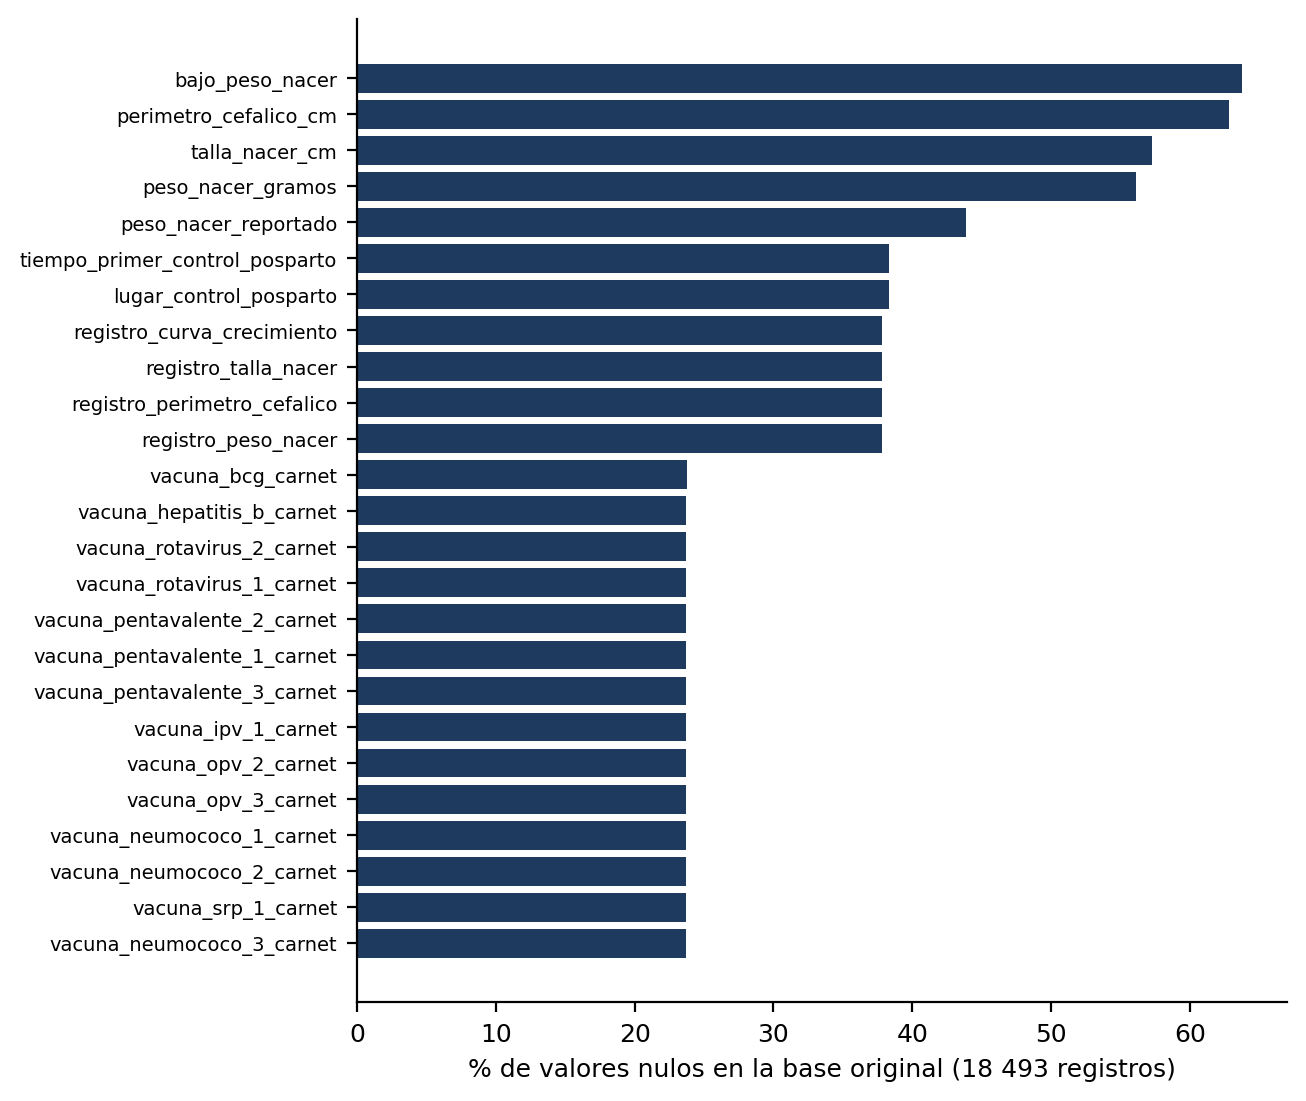
\includegraphics[width=0.8\textwidth]{figuras/anexo-nulos.png}
  \caption{Variables predictoras con mayor porcentaje de valores ausentes en la base original. Elaboración propia.}
  \label{fig:nulos}
\end{figure}

\section*{G.2 Distribución de variables numéricas}
\begin{figure}[H]
  \centering
  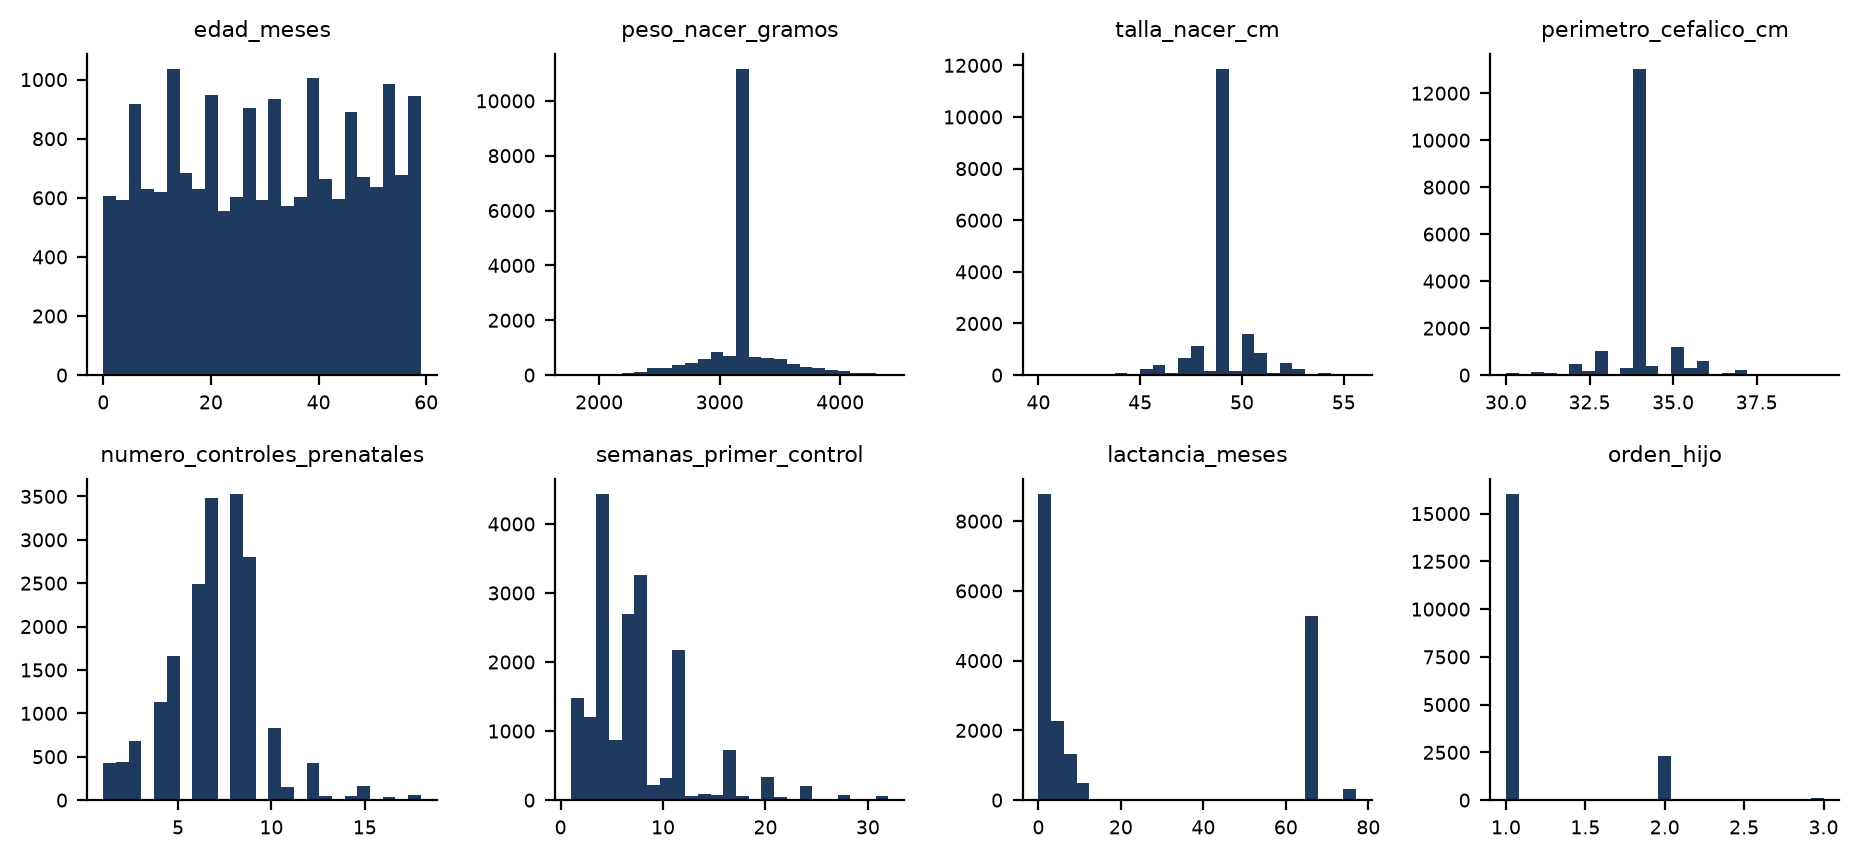
\includegraphics[width=\textwidth]{figuras/anexo-histogramas.png}
  \caption{Histogramas de variables numéricas seleccionadas (sin el 0.5\,\% de valores extremos en cada cola). Elaboración propia.}
  \label{fig:histogramas}
\end{figure}

\section*{G.3 Prevalencia por categoría}
La Figura~\ref{fig:prevcat} muestra la prevalencia muestral de desnutrición crónica según variables categóricas seleccionadas (categorías con al menos 30 registros; la línea roja indica la prevalencia global de \SI{24.7}{\percent}) y la Tabla~\ref{tab:prevcat} los valores. Son prevalencias sin ponderar y asociaciones descriptivas, no efectos causales.

\begin{figure}[H]
  \centering
  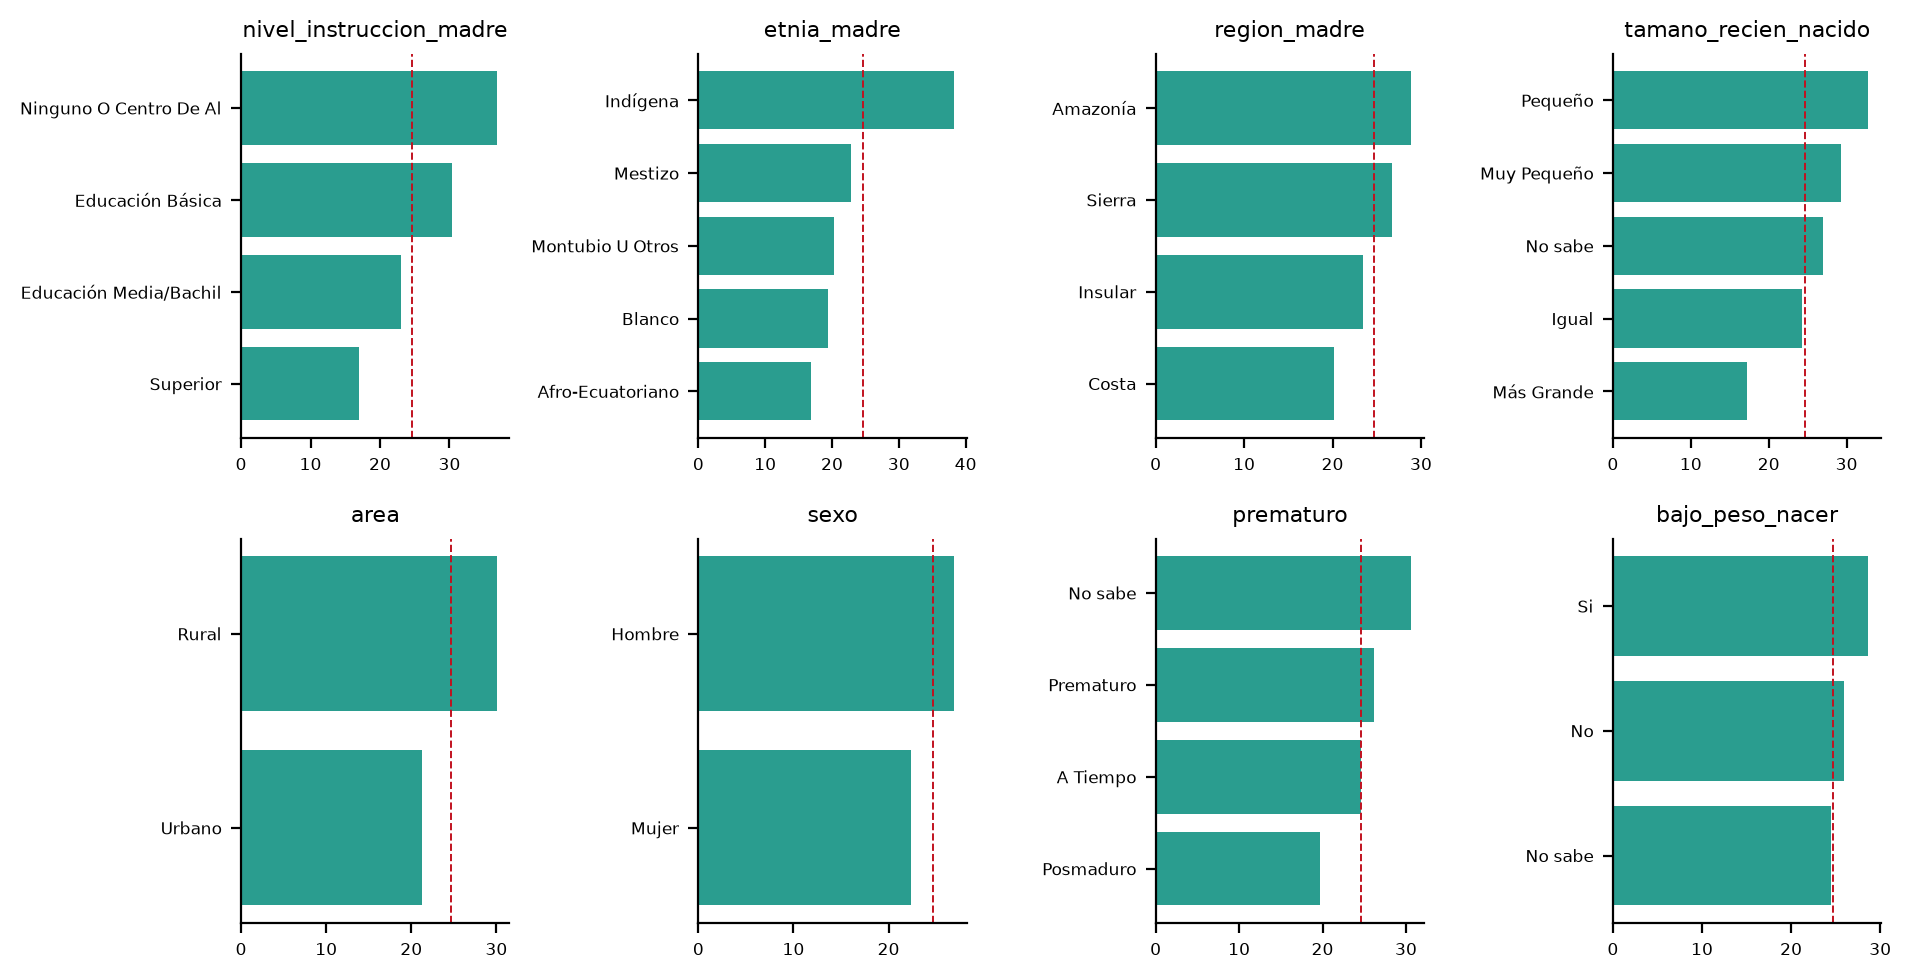
\includegraphics[width=\textwidth]{figuras/anexo-prevalencia-categorias.png}
  \caption{Prevalencia muestral de desnutrición crónica por categoría. Elaboración propia.}
  \label{fig:prevcat}
\end{figure}

\begingroup
\scriptsize\setlength{\tabcolsep}{4pt}\arrayrulecolor{black!55}\renewcommand{\arraystretch}{1.1}
\begin{longtable}{|p{4.4cm}|p{5.6cm}|r|r|}
  \caption{Prevalencia muestral de desnutrición crónica por categoría (sin ponderar).}
  \label{tab:prevcat}\\ \hline
  \enc{Variable} & \enc{Categoría} & \enc{n} & \enc{Prevalencia (\%)} \\ \hline
  \endfirsthead
  \tablacont{4}\hline
  \enc{Variable} & \enc{Categoría} & \enc{n} & \enc{Prevalencia (\%)} \\ \hline
  \endhead
  \hline\endfoot
    \texttt{nivel\_instruccion\_madre} & Superior & 3710 & 17.0 \\ \hline
    \texttt{nivel\_instruccion\_madre} & Educación Media/Bachillerato & 7864 & 23.0 \\ \hline
    \texttt{nivel\_instruccion\_madre} & Educación Básica & 6696 & 30.4 \\ \hline
    \texttt{nivel\_instruccion\_madre} & Ninguno O Centro De Alfabetización & 223 & 36.8 \\ \hline
    \texttt{etnia\_madre} & Afro-Ecuatoriano & 756 & 16.8 \\ \hline
    \texttt{etnia\_madre} & Blanco & 226 & 19.5 \\ \hline
    \texttt{etnia\_madre} & Montubio U Otros & 805 & 20.2 \\ \hline
    \texttt{etnia\_madre} & Mestizo & 14056 & 22.9 \\ \hline
    \texttt{etnia\_madre} & Indígena & 2650 & 38.2 \\ \hline
    \texttt{region\_madre} & Costa & 6991 & 20.1 \\ \hline
    \texttt{region\_madre} & Insular & 371 & 23.5 \\ \hline
    \texttt{region\_madre} & Sierra & 7014 & 26.7 \\ \hline
    \texttt{region\_madre} & Amazonía & 4117 & 28.9 \\ \hline
    \texttt{tamano\_recien\_nacido} & Más Grande & 3267 & 17.2 \\ \hline
    \texttt{tamano\_recien\_nacido} & Igual & 10770 & 24.3 \\ \hline
    \texttt{tamano\_recien\_nacido} & No sabe & 946 & 27.0 \\ \hline
    \texttt{tamano\_recien\_nacido} & Muy Pequeño & 796 & 29.3 \\ \hline
    \texttt{tamano\_recien\_nacido} & Pequeño & 2714 & 32.8 \\ \hline
    \texttt{area} & Urbano & 11240 & 21.2 \\ \hline
    \texttt{area} & Rural & 7253 & 30.0 \\ \hline
    \texttt{sexo} & Mujer & 8981 & 22.3 \\ \hline
    \texttt{sexo} & Hombre & 9512 & 26.9 \\ \hline
    \texttt{prematuro} & Posmaduro & 442 & 19.7 \\ \hline
    \texttt{prematuro} & A Tiempo & 15853 & 24.6 \\ \hline
    \texttt{prematuro} & Prematuro & 2149 & 26.2 \\ \hline
    \texttt{prematuro} & No sabe & 49 & 30.6 \\ \hline
    \texttt{bajo\_peso\_nacer} & No sabe & 17001 & 24.5 \\ \hline
    \texttt{bajo\_peso\_nacer} & No & 920 & 26.0 \\ \hline
    \texttt{bajo\_peso\_nacer} & Si & 572 & 28.7 \\ \hline
\end{longtable}
\endgroup


%% ----------------------------------------------------------------- ANEXO H
\anexo{H}{Resultados Ampliados}

\section*{H.1 Modelos base: matrices de confusión}
\begin{table}[H]
  \caption{Conteos de la matriz de confusión de los modelos base (clase 1 = con desnutrición crónica).}
  \label{tab:conf4}
  \tablabase\footnotesize
  \begin{tabular}{|l|c|c|c|c|c|}
    \hline
    \enc{Modelo} & \enc{Umbral} & \enc{VP} & \enc{FN} & \enc{FP} & \enc{VN} \\ \hline
    Regresión logística & 0.50 & 557 & 355 & 994 & 1793 \\ \hline
    Regresión logística & 0.47 & 614 & 298 & 1187 & 1600 \\ \hline
    Árbol de decisión & 0.50 & 274 & 638 & 634 & 2153 \\ \hline
    Árbol de decisión & 0.05 & 274 & 638 & 634 & 2153 \\ \hline
    Random Forest & 0.50 & 23 & 889 & 11 & 2776 \\ \hline
    Random Forest & 0.23 & 670 & 242 & 1336 & 1451 \\ \hline
    XGBoost & 0.50 & 385 & 527 & 634 & 2153 \\ \hline
    XGBoost & 0.24 & 747 & 165 & 1787 & 1000 \\ \hline
  \end{tabular}
\end{table}


\begin{figure}[H]
  \centering
  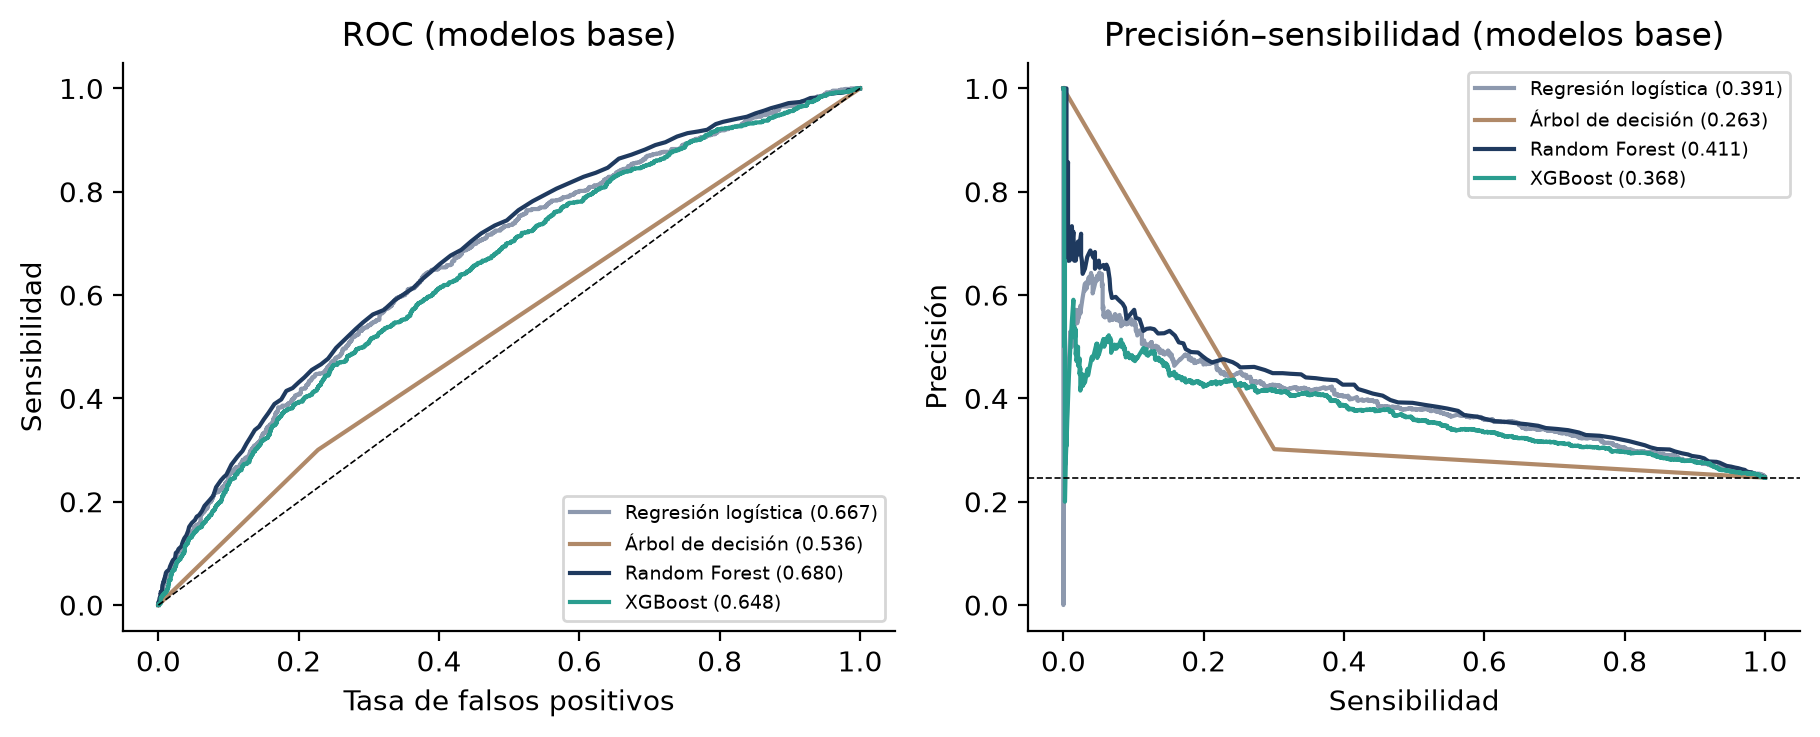
\includegraphics[width=\textwidth]{figuras/anexo-curvas-4modelos.png}
  \caption{Curvas ROC y de precisión--sensibilidad de los cuatro modelos base en el conjunto de prueba. Elaboración propia.}
  \label{fig:curvas4}
\end{figure}

\section*{H.2 Sensibilidad al umbral}
\begin{table}[H]
  \caption{Desempeño del modelo final en la prueba según el umbral de decisión.}
  \label{tab:umbrales}
  \tablabase\footnotesize
  \begin{tabular}{|l|c|c|c|c|c|c|}
    \hline
    \enc{Umbral} & \enc{Sens.} & \enc{Espec.} & \enc{Prec.} & \enc{F1} & \enc{Ex. bal.} & \enc{Alertas} \\ \hline
    0.3 & 0.959 & 0.110 & 0.261 & 0.410 & 0.535 & 3355 \\ \hline
    0.42 & 0.693 & 0.550 & 0.335 & 0.452 & 0.621 & 1887 \\ \hline
    0.5 & 0.386 & 0.826 & 0.421 & 0.403 & 0.606 & 837 \\ \hline
    0.6 & 0.106 & 0.968 & 0.524 & 0.177 & 0.537 & 185 \\ \hline
  \end{tabular}
\end{table}


\section*{H.3 Calibración}
\begin{table}[H]
  \caption{Calibración por deciles de probabilidad predicha (conjunto de prueba).}
  \label{tab:calib}
  \tablabase\footnotesize
  \begin{tabular}{|l|c|c|}
    \hline
    \enc{Decil} & \enc{Probabilidad media} & \enc{Proporción observada} \\ \hline
    1 & 0.264 & 0.105 \\ \hline
    2 & 0.326 & 0.103 \\ \hline
    3 & 0.358 & 0.165 \\ \hline
    4 & 0.384 & 0.203 \\ \hline
    5 & 0.410 & 0.206 \\ \hline
    6 & 0.435 & 0.208 \\ \hline
    7 & 0.462 & 0.268 \\ \hline
    8 & 0.493 & 0.346 \\ \hline
    9 & 0.532 & 0.357 \\ \hline
    10 & 0.608 & 0.505 \\ \hline
  \end{tabular}
\end{table}

El error cuadrático de Brier es 0.205 (referencia con la prevalencia como única predicción: 0.186). \begin{figure}[H]
  \centering
  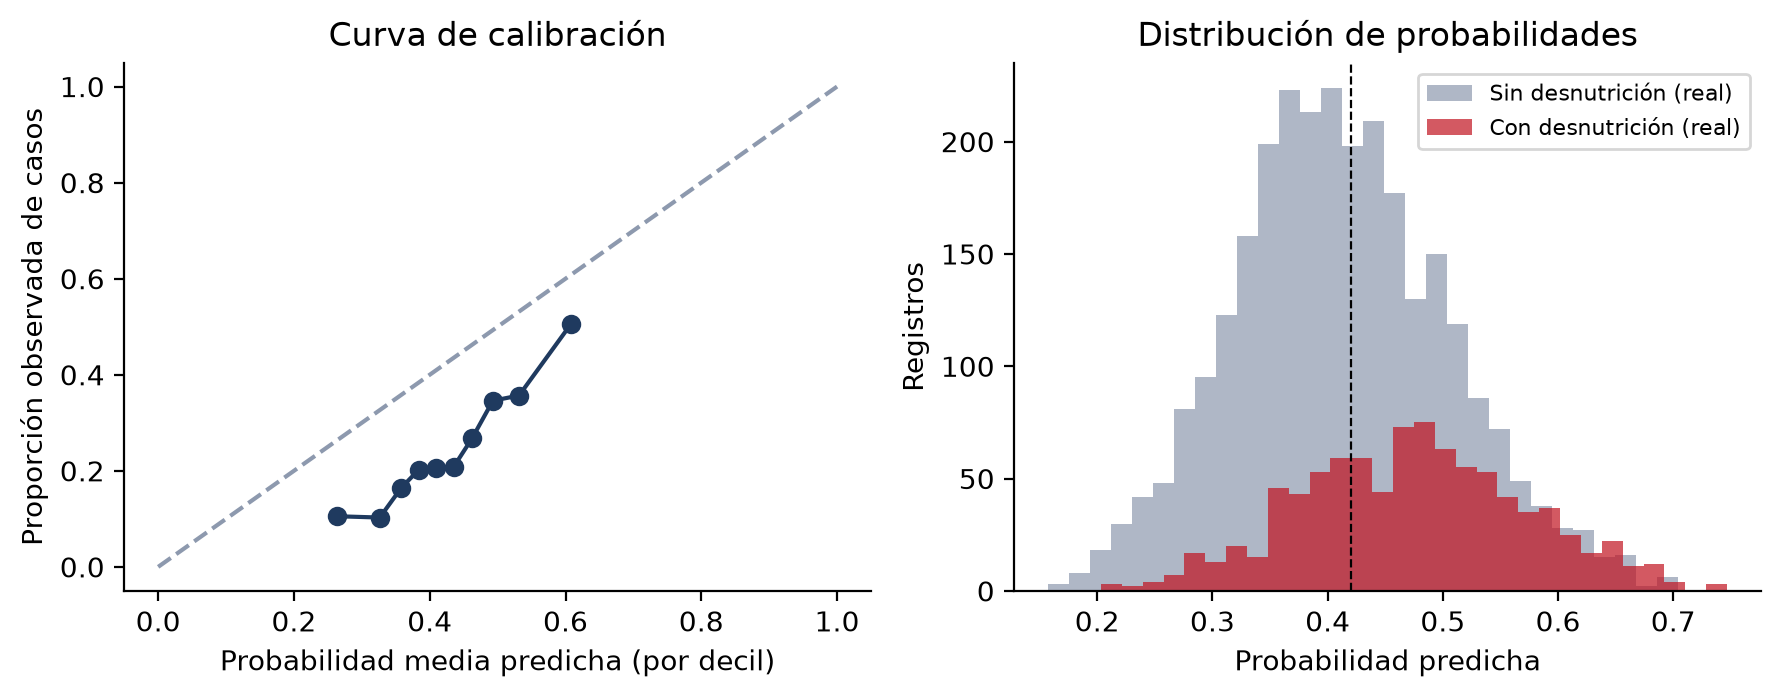
\includegraphics[width=0.95\textwidth]{figuras/anexo-calibracion.png}
  \caption{Curva de calibración y distribución de probabilidades predichas. Elaboración propia.}
  \label{fig:calibracion}
\end{figure}


\section*{H.4 Desempeño por subgrupos (detalle)}
\begin{table}[H]
  \caption{Desempeño por subgrupos en la prueba (umbral 0.42; IC de Wilson para la sensibilidad).}
  \label{tab:subgrupos}
  \tablabase\scriptsize
  \begin{tabular}{|l|c|c|c|c|c|c|c|}
    \hline
    \enc{Ámbito} & \enc{Variable} & \enc{Valor} & \enc{n} & \enc{Casos} & \enc{Sensibilidad (IC 95\,\%)} & \enc{Espec.} & \enc{ROC-AUC} \\ \hline
    Nacional & area & Rural & 1456 & 432 & 0.880 (0.846--0.907) & 0.312 & 0.682 \\ \hline
    Nacional & area & Urbano & 2243 & 480 & 0.525 (0.480--0.569) & 0.687 & 0.656 \\ \hline
    Tungurahua & area & Rural & 26 & 14 & 0.786 (0.524--0.924) & 0.083 & 0.423 \\ \hline
    Tungurahua & area & Urbano & 86 & 21 & 0.619 (0.409--0.792) & 0.662 & 0.686 \\ \hline
    Nacional & sexo & Hombre & 1904 & 510 & 0.720 (0.679--0.757) & 0.514 & 0.672 \\ \hline
    Nacional & sexo & Mujer & 1795 & 402 & 0.659 (0.612--0.704) & 0.586 & 0.679 \\ \hline
    Tungurahua & sexo & Hombre & 46 & 13 & 0.769 (0.497--0.918) & 0.424 & 0.608 \\ \hline
    Tungurahua & sexo & Mujer & 66 & 22 & 0.636 (0.430--0.803) & 0.682 & 0.718 \\ \hline
    Nacional & edad (meses) & 0-5 & 294 & 64 & 0.609 (0.487--0.719) & 0.504 & 0.597 \\ \hline
    Nacional & edad (meses) & 6-11 & 370 & 85 & 0.659 (0.553--0.751) & 0.540 & 0.650 \\ \hline
    Nacional & edad (meses) & 12-23 & 762 & 259 & 0.892 (0.848--0.924) & 0.247 & 0.654 \\ \hline
    Nacional & edad (meses) & 24-35 & 747 & 209 & 0.751 (0.688--0.805) & 0.493 & 0.667 \\ \hline
    Nacional & edad (meses) & 36-59 & 1526 & 295 & 0.505 (0.448--0.562) & 0.709 & 0.663 \\ \hline
    Tungurahua & edad (meses) & 12-23 & 26 & 10 & 0.800 (0.490--0.943) & 0.250 & 0.600 \\ \hline
    Tungurahua & edad (meses) & 24-35 & 21 & 8 & 0.750 (0.409--0.929) & 0.462 & 0.519 \\ \hline
    Tungurahua & edad (meses) & 36-59 & 54 & 13 & 0.538 (0.291--0.768) & 0.732 & 0.704 \\ \hline
  \end{tabular}
\end{table}


\section*{H.5 Hiperparámetros del modelo final}
\begin{table}[H]
  \caption{Hiperparámetros efectivos del Random Forest final.}
  \label{tab:hiper}
  \tablabase\scriptsize
  \begin{tabular}{|p{3.4cm}|p{2.6cm}|p{3.4cm}|p{2.6cm}|}
    \hline
    \enc{Parámetro} & \enc{Valor} & \enc{Parámetro} & \enc{Valor} \\ \hline
    \texttt{bootstrap} & True & \texttt{min\_samples\_split} & 2 \\ \hline
    \texttt{ccp\_alpha} & 0.0 & \texttt{min\_weight\_fraction\_leaf} & 0.0 \\ \hline
    \texttt{class\_weight} & balanced & \texttt{monotonic\_cst} & None \\ \hline
    \texttt{criterion} & gini & \texttt{n\_estimators} & 300 \\ \hline
    \texttt{max\_depth} & 20 & \texttt{n\_jobs} & None \\ \hline
    \texttt{max\_features} & sqrt & \texttt{oob\_score} & False \\ \hline
    \texttt{max\_leaf\_nodes} & None & \texttt{random\_state} & 42 \\ \hline
    \texttt{max\_samples} & None & \texttt{verbose} & 0 \\ \hline
    \texttt{min\_impurity\_decrease} & 0.0 & \texttt{warm\_start} & False \\ \hline
    \texttt{min\_samples\_leaf} & 10 &  &  \\ \hline
  \end{tabular}
\end{table}


\section*{H.6 Importancia de variables (30 principales)}
\begin{table}[H]
  \caption{Las 30 variables con mayor importancia (suma de sus columnas codificadas, \% del total).}
  \label{tab:top30}
  \tablabase\scriptsize
  \begin{tabular}{|c|p{6.4cm}|c|}
    \hline
    \enc{N.º} & \enc{Variable} & \enc{Importancia (\%)} \\ \hline
    1 & \texttt{edad\_meses} & 4.50 \\ \hline
    2 & \texttt{factor\_expansion} (diseño muestral) & 3.70 \\ \hline
    3 & \texttt{grupo\_edad\_meses} & 3.67 \\ \hline
    4 & \texttt{estrato} (diseño muestral) & 3.64 \\ \hline
    5 & \texttt{nivel\_instruccion\_madre} & 3.21 \\ \hline
    6 & \texttt{provincia} & 3.09 \\ \hline
    7 & \texttt{tamano\_recien\_nacido} & 2.75 \\ \hline
    8 & \texttt{peso\_nacer\_gramos} & 2.69 \\ \hline
    9 & \texttt{etnia\_madre} & 2.63 \\ \hline
    10 & \texttt{area} & 2.14 \\ \hline
    11 & \texttt{numero\_controles\_prenatales} & 2.07 \\ \hline
    12 & \texttt{region\_madre} & 2.02 \\ \hline
    13 & \texttt{semanas\_primer\_control} & 2.01 \\ \hline
    14 & \texttt{sexo} & 1.95 \\ \hline
    15 & \texttt{talla\_nacer\_cm} & 1.94 \\ \hline
    16 & \texttt{controles\_0\_1\_anio} & 1.94 \\ \hline
    17 & \texttt{lugar\_parto} & 1.75 \\ \hline
    18 & \texttt{tipo\_parto} & 1.66 \\ \hline
    19 & \texttt{lactancia\_meses} & 1.64 \\ \hline
    20 & \texttt{controles\_1\_2\_anios} & 1.59 \\ \hline
    21 & \texttt{personal\_parto} & 1.47 \\ \hline
    22 & \texttt{controles\_2\_5\_anios} & 1.45 \\ \hline
    23 & \texttt{lugar\_control\_prenatal} & 1.43 \\ \hline
    24 & \texttt{tiempo\_primer\_control\_nino} & 1.32 \\ \hline
    25 & \texttt{examen\_sifilis\_embarazo} & 1.30 \\ \hline
    26 & \texttt{vitamina\_a\_12\_meses} & 1.28 \\ \hline
    27 & \texttt{perimetro\_cefalico\_cm} & 1.23 \\ \hline
    28 & \texttt{corte\_oportuno\_cordon} & 1.21 \\ \hline
    29 & \texttt{desparasitacion\_6\_meses} & 1.11 \\ \hline
    30 & \texttt{control\_posparto} & 1.09 \\ \hline
  \end{tabular}
\end{table}


%% ----------------------------------------------------------------- ANEXO I
\anexo{I}{Código Esencial}

Se incluye el código esencial del pipeline y del servicio. El resto está en el repositorio (Anexo~E). Los comentarios conservan la redacción original del código.

\section*{I.1 Construcción de la base sin fuga (\texttt{build\_clean\_dataset.py})}
\lstinputlisting[language=Python,basicstyle=\ttfamily\scriptsize,frame=single]{anexos/codigo/build_clean_dataset.py}

\section*{I.2 Partición reproducible (\texttt{split\_dataset.py})}
\lstinputlisting[language=Python,basicstyle=\ttfamily\scriptsize,frame=single]{anexos/codigo/split_dataset.py}

\section*{I.3 Revisión de fuga por variable (\texttt{leakage\_screen.py})}
\lstinputlisting[language=Python,basicstyle=\ttfamily\scriptsize,frame=single]{anexos/codigo/leakage_screen.py}

\section*{I.4 Preprocesamiento, modelos, umbral y evaluación (\texttt{entrenar\_modelo.py}, extracto)}
\lstinputlisting[language=Python,basicstyle=\ttfamily\scriptsize,frame=single]{anexos/codigo/entrenar_extracto.py}

\section*{I.5 Servicio de predicción (\texttt{predictor.py})}
\lstinputlisting[language=Python,basicstyle=\ttfamily\scriptsize,frame=single]{anexos/codigo/predictor.py}

\section*{I.6 Ruta de predicción individual (\texttt{main.py}, extracto)}
\lstinputlisting[language=Python,basicstyle=\ttfamily\scriptsize,frame=single]{anexos/codigo/main_predict.py}


\end{document}
